% Este documento tem a ver com as partes do LIVRO. 

% Tamanhos
% \tiny
% \scriptsize
% \footnotesize
% \small 
% \normalsize
% \large 
% \Large 
% \LARGE 
% \huge
% \Huge

% Posicionamento
% \centering 
% \raggedright
% \raggedleft
% \vfill 
% \hfill 
% \vspace{Xcm}   % Colocar * caso esteja no começo de uma página. Ex: \vspace*{...}
% \hspace{Xcm}

% Estilo de página
% \thispagestyle{<<nosso>>}
% \thispagestyle{empty}
% \thispagestyle{plain}  (só número, sem cabeço)
% https://www.overleaf.com/learn/latex/Headers_and_footers

% Compilador que permite usar fonte de sistema: xelatex, lualatex
% Compilador que não permite usar fonte de sistema: latex, pdflatex

% Definindo fontes
% \setmainfont{Times New Roman}  % Todo o texto
% \newfontfamily\avenir{Avenir}  % Contexto

\begingroup\thispagestyle{empty}

\begin{textblock*}{2.625in}(0pt,0pt)%
\vspace*{-3.5cm}
%\hspace*{-4cm}
\includegraphics[scale=1]{../watermarks/front5ano.pdf}
\end{textblock*}
                
              \vspace*{\fill}
              \begin{center}
              {\HUGE\textbf{Revisa SAEB}}\bigskip

              {\LARGE\textbf{2º ano: Matemática}}

              \bigskip
              \bigskip
              \bigskip

              {\Large
                            AUTORIA

                            }
              \end{center}
              \vspace*{\fill}

\endgroup
\pagebreak       % [Frontistício]
%\newcommand{\linhalayout}[2]{{\tiny\textbf{#1}\quad#2\par}}
\newcommand{\linha}[2]{\ifdef{#2}{\linhalayout{#1}{#2}}{}}

\begingroup\tiny
\parindent=0cm
\thispagestyle{empty}

\textbf{Gerência editorial}\quad			 {Ana Mortara}\\
\textbf{Assistência editorial}\quad			 {Paula Dias}\\
\textbf{Assistência administrativa editorial}\quad {Gisele Cerchiaro}\\

\hspace{-5pt}\begin{tabular}{ll}
\textbf{Elaboração de conteúdo} & Abraão Augusto (Língua Portuguesa),	\\
								& Alessandra Domingues Juliano (Língua Portuguesa),	\\
								& Ana Paula Souza Rios (Língua Portuguesa),	\\
								& André Sanchez Astorino (Língua Portuguesa e Língua Inglesa),	\\
								& Clarissa Ayres Mendes (Língua Portuguesa),	\\
								& Eduardo Toniolo Campos (Matemática),	\\
								& Fernanda Dobashi (Língua Portuguesa),	\\
								& Guilherme Salles (Ciências Humanas),	\\
								& Letícia Leme (Ciências Humanas),	\\
								& Lucas Della Santina (Educação Física),	\\
								& Pilar Espí (Arte),	\\
								& Renata Cândido Carvalho (Ciências da Natureza),	\\
								& Thiago Figueiredo (Matemática),	\\
								& Victor Marques (Ciências da Natureza)	\\
\end{tabular}


\textbf{Edição}\quad	 {Carlos Rogério Duarte Barreiros, Fábia Alvim, Felipe Augusto Neves Silva}\\
\textbf{Preparação e revisão}\quad			 {Saíra Editorial}\\
\textbf{Coordenação de arte}\quad			 {Jorge Sallum}\\
\textbf{Editoração eletrônica}\quad			 {Paulo Henrique Pompermaier}\\
\textbf{Pesquisa iconográfica}\quad			 {Margarita Veloso}\\
\textbf{Projeto gráfico e capa}\quad		 {Luísa Marcelino}\\
\textbf{Código}\quad {\ifdef{\RevisionInfo{}}{\RevisionInfo{} (\today, \currenttime)}{001}\medskip}

\noindent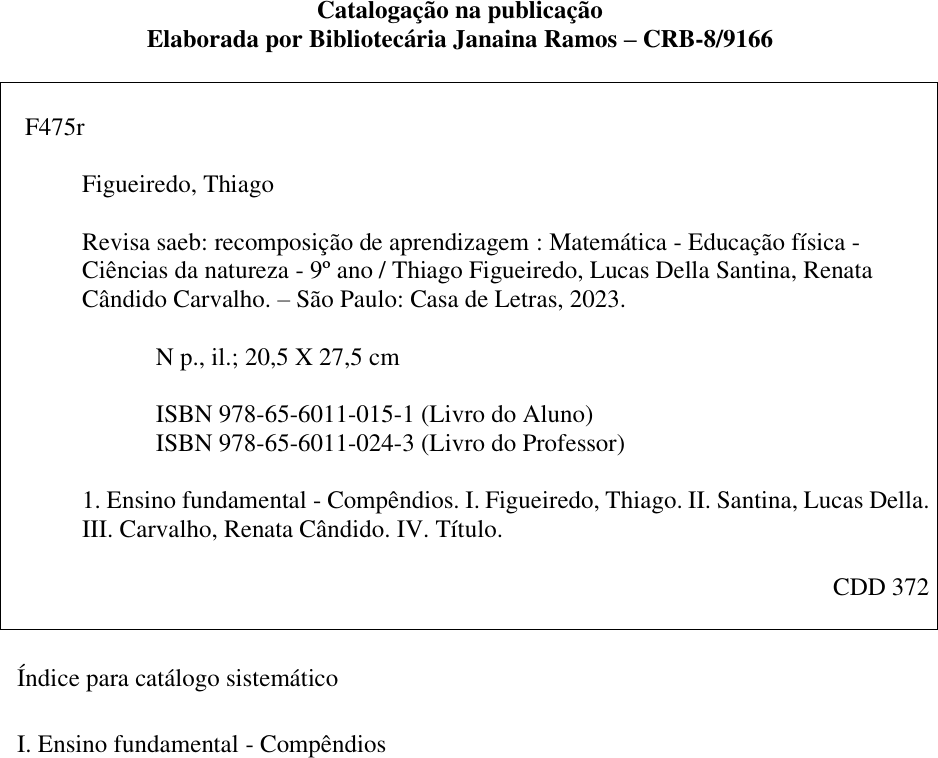
\includegraphics[width=.5\textwidth]{../fichas/9MAT.png}

\vfill

\textsc{casa de letras e gráfica ltda.}\\
Rua Fradique Coutinho, 1139, andar 2, sala 2\\
CEP 05416--011 -- São Paulo/\textsc{sp}, Brasil\\
Telefone: (11) 3914--7790\\\smallskip
www.casadeletras.com.br\\

\endgroup
\pagebreak
     % [Créditos]
% nothing			is level -3
% \book				is level -2
% \part				is level -1
% \chapter 			is level 0
% \section 			is level 1
% \subsection 		is level 2
% \subsubsection 	is level 3
% \paragraph 		is level 4
% \subparagraph 	is level 5
\setcounter{secnumdepth}{-2}
\setcounter{tocdepth}{0}

% \renewcommand{\contentsname}{Índex} 	% Trocar nome do sumário para 'Índex'
%\ifodd\thepage\relax\else\blankpage\fi 	% Verifica se página é par e coloca página branca
%\tableofcontents*

\pagebreak
{\begingroup\mbox{}\pagestyle{empty}
\pagestyle{empty} 
% \renewcommand{\contentsname}{Índex} 	% Trocar nome do sumário para 'Índex'
%\ifodd\thepage\relax\else\blankpage\fi 	% Verifica se página é par e coloca página branca
\addtocontents{toc}{\protect\thispagestyle{empty}}
%\addtocontents{toc}{\vspace*{-.1cm}}
\tableofcontents*\clearpage\endgroup}

\pagestyle{por}
\chapter[O alfabeto, as vogais e as consoantes]{\Large O alfabeto, as vogais e as consoantes}
\markboth{Módulo 1}{}

\colorsec{Habilidade do SAEB}

\begin{itemize}
\item Relacionar elementos sonoros das palavras com sua representação escrita.
\end{itemize}

\colorsec{Habilidade da BNCC}

\begin{itemize}
\item EF02LP03.
\end{itemize}

\conteudo{Para escrever as palavras, usamos as \textbf{letras}. 
Juntas, elas compõem o \textbf{alfabeto}, que é formado por 26 letras. 

As \textbf{vogais} são \textit{a, e, i, o, u}, e as outras letras são
chamadas de \textbf{consoantes}. Veja:

\begin{myquote}
b c d f g h j k l m n p q r s t v w x y z
\end{myquote}

Cada letra possui um nome e um som, que, quando estão juntos, podem
formar muitas palavras.

\begin{longtable}[]{@{}llllll@{}}
\toprule
\textbf{PATO} & \textbf{VACA} & \textbf{BOLA} & \textbf{TATU} &
\textbf{FADA} & \textbf{DOCE}\tabularnewline
\bottomrule
\end{longtable}

A letra C pode apresentar dois sons diferentes de acordo com a vogal que
acompanha. Por exemplo: junto com as vogais A, O e U, apresenta o som de 
/k/; junto com E e I apresenta o som de /s/.
}
 
%Felipe: precisamos padronizar como vamos grafar as letras e os fonemas, como ocorreu na frase acima. (Rogério, 13/3/23, 14h31)

\conteudo{
Algumas palavras com o som de /k/ também podem ser escritas com Q,
mas vale lembrar que o Q vem sempre acompanhado de U e de mais uma
vogal, e é esta última vogal que vai marcar o som da sílaba. Observe:

\begin{center}
\begin{tabular}{l}
\hline
\textbf{PALAVRAS C COM SOM DE /K/} \\ \hline
\textbf{CUCA} \\
\textbf{CASA} \\
\textbf{COCO} \\ \hline
\textbf{PALAVRAS C COM SOM DE /S/} \\ \hline
\textbf{CEBOLA} \\
\textbf{CINCO} \\
\textbf{CISNE} \\ \hline
\textbf{PALAVRAS COM QU} \\ \hline
\textbf{QUEIJO} \\
\textbf{QUILO} \\
\textbf{QUERO} \\
\textbf{QUIBE}
\end{tabular}
\end{center}

Veja a grafia dessas palavras.

\begin{myquote}
TATU \hspace{2cm}  GALO 
\end{myquote}

Na grafia das palavras com as vogais O e U, o O no final de palavras é
fraco, e o U é sempre forte.

\begin{quote}
A letra /k/ é usada apenas em situações como nomes de
pessoas, como Kátia, e palavras estrangeiras como
\textit{ketchup, kit, kibon} e \textit{kaiser}.
\end{quote}
}

\pagebreak
\colorsec{Atividades}

\num{1} Complete os nomes das figuras com as letras que estão faltando.

\begin{figure}[htpb!]
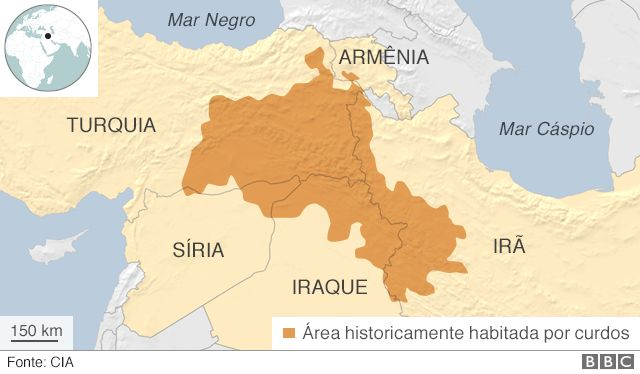
\includegraphics[width=.5\textwidth]{media/image1.jpeg}
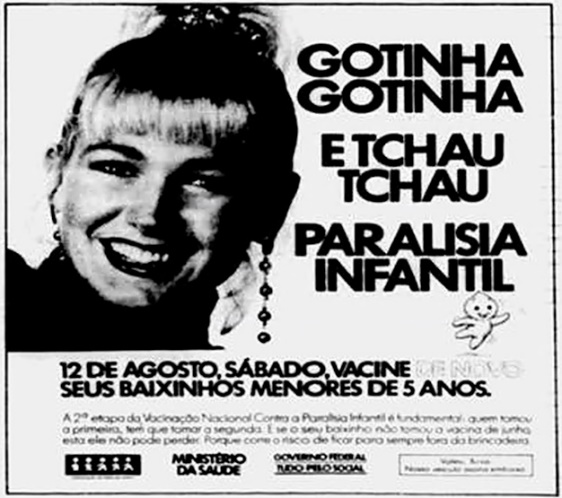
\includegraphics[width=.5\textwidth]{media/image2.jpeg}
\end{figure}

T \reduline{A} P \reduline{E} T \reduline{E}\hspace{6cm} C \reduline{A} V \reduline{A} L \reduline{O}


\begin{figure}[htpb!]
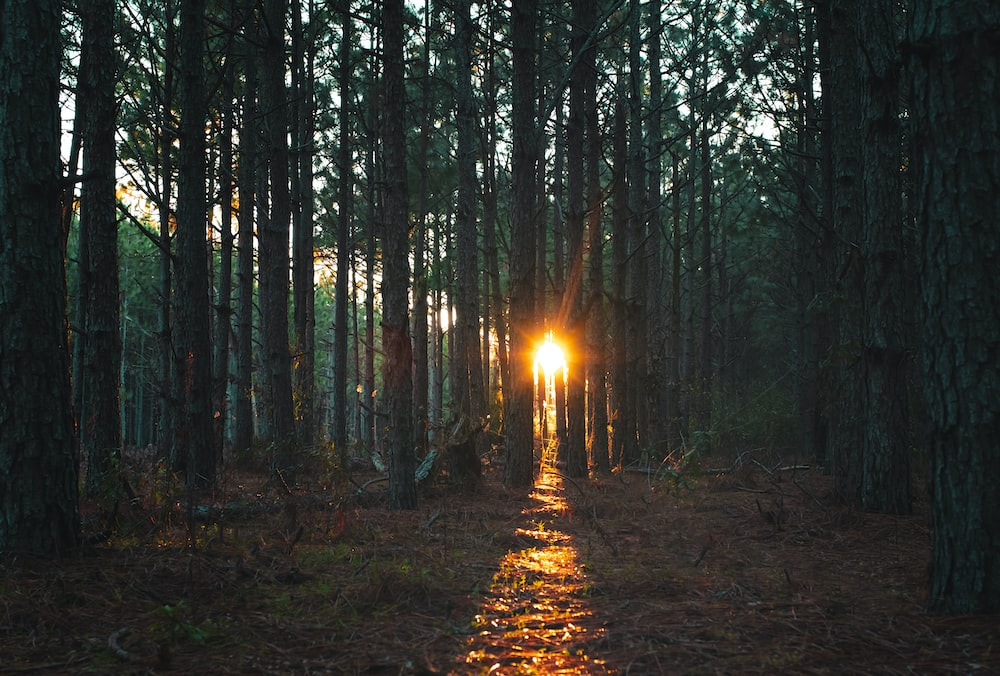
\includegraphics[width=.5\textwidth]{media/image3.jpeg}
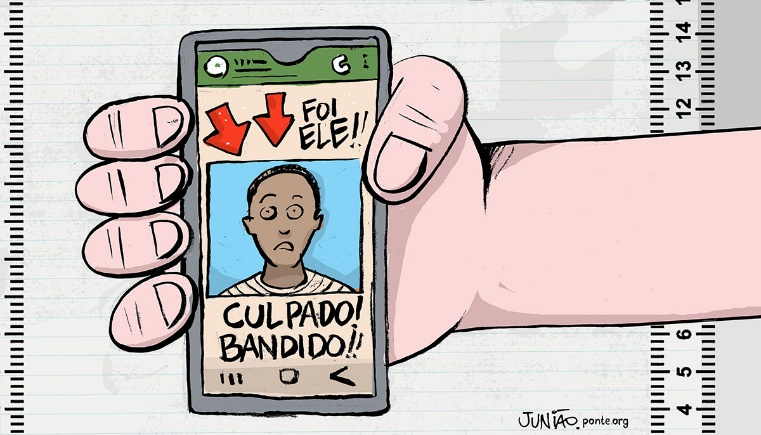
\includegraphics[width=.5\textwidth]{media/image4.jpeg}
\end{figure}

\reduline{E} STR \reduline{E} L \reduline{A} \hspace{6cm} P \reduline{O} RT \reduline{A}

\pagebreak
Você completou as palavras com

\begin{boxlist}
\boxitem{\white{X}} Vogais 

\boxitem{\white{X}} Consoantes
\end{boxlist}

%\coment{Apresente as vogais em cartaz. Pergunte o nome dos objetos representados nas imagens e, em seguida, convide as crianças para montar as palavras no alfabeto móvel para identificar as letras faltantes.}

\num{2} Complete o alfabeto com as letras que estão faltado.

\begin{center}
\Large
\begin{tabular}{|l|l|llllll}
\hline
\textbf{A} & \rosa{B} & \multicolumn{1}{l|}{\rosa{C}} & \multicolumn{1}{l|}{\rosa{D}} & \multicolumn{1}{l|}{\textbf{E}} & \multicolumn{1}{l|}{\rosa{F}} & \multicolumn{1}{l|}{\rosa{G}} & \multicolumn{1}{l|}{\rosa{H}} \\ \hline
\textbf{I} & \rosa{J} & \multicolumn{1}{l|}{\rosa{K}} & \multicolumn{1}{l|}{\rosa{L}} & \multicolumn{1}{l|}{\rosa{M}} & \multicolumn{1}{l|}{\rosa{N}} & \multicolumn{1}{l|}{\textbf{O}} & \multicolumn{1}{l|}{\rosa{P}} \\ \hline
\rosa{Q} & \rosa{R} & \multicolumn{1}{l|}{\rosa{S}} & \multicolumn{1}{l|}{\rosa{T}} & \multicolumn{1}{l|}{\textbf{U}} & \multicolumn{1}{l|}{\rosa{V}} & \multicolumn{1}{l|}{\rosa{W}} & \multicolumn{1}{l|}{\rosa{X}} \\ \hline
\rosa{Y} & \rosa{Z} & \textbf{} & \textbf{} & \textbf{} & \textbf{} & \textbf{} & \textbf{} \\ \cline{1-2}
\end{tabular}
\end{center}

Você completou as palavras com:

\begin{boxlist}
\boxitem{\white{X}} Vogais 

\boxitem{\white{X}} Consoantes
\end{boxlist}

%\coment{Leve o alfabeto móvel para sala e convide os alunos para organizar as letras na ordem certa. Em seguida, oriente-os a preencher o quadro; depois ajude a separar vogais e consoantes.}

\num{3} Leia o poema.

\textbf{A vaca Filomena e a formiga Violeta}


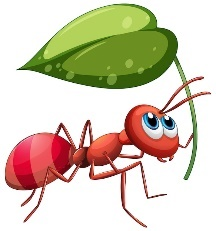
\includegraphics[width=.2\textwidth]{media/image5.jpeg}

\includegraphics[width=.3\textwidth]{media/image6.jpeg}

\begin{verse}
A vaca Filomena\\
mora na vila formosa.\\
A formiga Violeta\\
mora na cerca cor de rosa.

\pagebreak
A vaca Filomena\\
come as uvas da parreira.\\
A formiga Violeta\\
acha isto uma besteira.
\end{verse}

\fonte{Isabel Cristina Silveira Soares. https://seceducacao.padua.rj.gov.br/wp-content/uploads/2021/05/3o-ano-Ling.-Portuguesa-ATIV.17.pdf.
Acesso 28 de Fev 2023.}

Encontre e pinte no texto todas as palavras iniciadas com F e V. 
Depois escreva abaixo as palavras que encontrou.

\reduline{As palavras encontradas são as seguintes: vaca, Filomena, vila,
formosa, formiga, violeta.
Leve as palavras \textit{vaca} e \textit{formiga} em uma caixinha e
apresente-as para as crianças. Faça a leitura das palavras e estimule 
questionamentos sobre esses animais: os alunos sabem como eles são?
Onde esses animais vivem? Que sons eles emitem? Faça com os
alunos a leitura do poema e oriente a localização das palavras iniciadas
com as consoantes V e F.\hfill}

\num{4} Complete os espaços a seguir com as letras iniciais das palavras
\textit{violeta} e \textit{filomena}.

%\coment{Leve as palavras Violeta e Filomena em um cartaz. Explore a letra inicial e o som da letra nas palavras.}

\begin{figure}[htpb!]

\includegraphics[width=.3\textwidth]{media/image7.jpeg}

\includegraphics[width=.3\textwidth]{media/image8.jpeg}

\includegraphics[width=.3\textwidth]{media/image9.jpeg}
\end{figure}

\reduline{F} ACA \hspace{4cm} \reduline{F} ADA \hspace{3cm} \reduline{V} ELA

\pagebreak
\begin{figure}[htpb!]
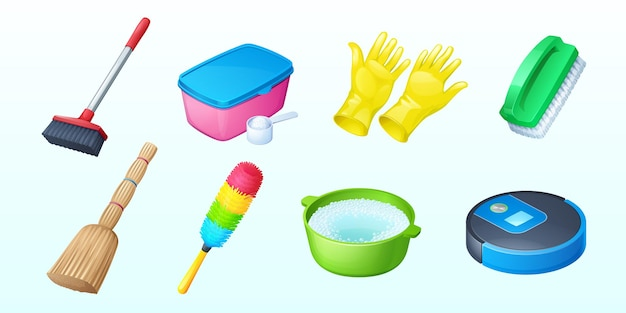
\includegraphics[width=.3\textwidth]{media/image10.jpeg}
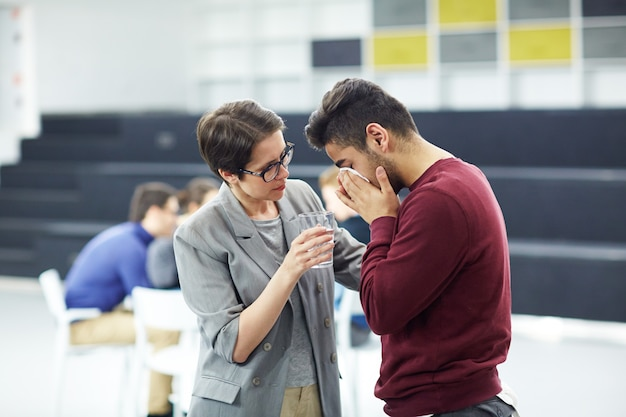
\includegraphics[width=.3\textwidth]{media/image11.jpeg}

\includegraphics[width=.3\textwidth]{media/image12.jpeg}
\end{figure}

 \reduline{V} ASSOURA \hspace{4cm} \reduline{F} OGO \hspace{3cm} \reduline{F} IVELA

\begin{figure}[htpb!]
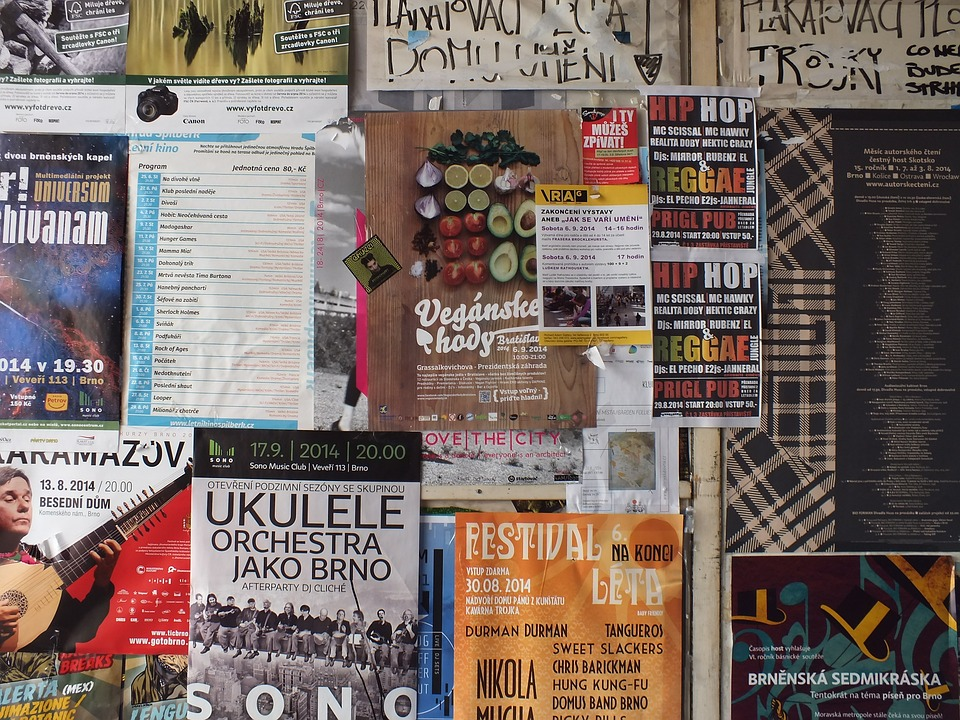
\includegraphics[width=.3\textwidth]{media/image13.jpeg}

\includegraphics[width=.3\textwidth]{media/image14.jpeg}
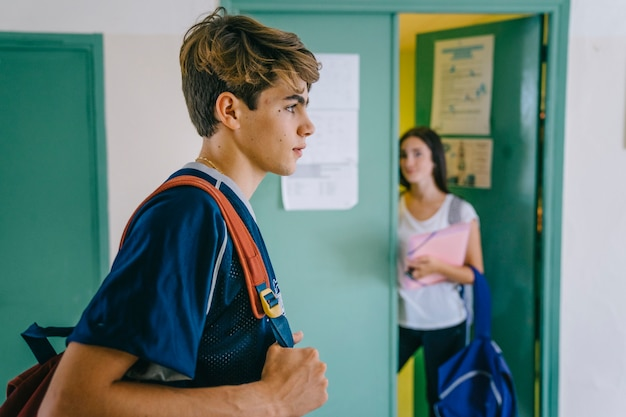
\includegraphics[width=.3\textwidth]{media/image15.jpeg}
\end{figure}

\reduline{F} LOR \hspace{4cm} \reduline{F} OGUETE \hspace{3cm} SOR \reduline{V} ETE


\num{5} Pinte as iniciais de cada palavra.

%\coment{Leve para sala palavras iniciadas pelas letras T, D, F, V, B, P. Convide as crianças para fazer a leitura, identificado o som das letras iniciais e finais, e quantidade de sílabas. Também é possível trabalhar a função social da escrita das palavras}.

\begin{center}
\begin{tabular}{|c|c|c|c|c|}
\hline
\textbf{VACINA} & F & T & D & \rosa{V} \\ \hline
\textbf{TESOURA} & P & D & \rosa{T} & F \\ \hline
\textbf{VASSOURA} & B & T & \rosa{V} & F \\ \hline
\textbf{FACA} & V & \rosa{F} & D & T \\ \hline
\textbf{DEDO} & T & V & F & \rosa{D} \\ \hline
\textbf{PANELA} & V & T & \rosa{P} & B \\ \hline
\textbf{DOMINÓ} & B & \rosa{D} & T & P \\ \hline
\textbf{BONECA} & F & P & \rosa{B} & D \\ \hline
\end{tabular}
\end{center}

\pagebreak
\num{6} Numere os desenhos conforme os números das palavras.

%\coment{Faça leitura das palavras com as crianças, de modo que elas identifiquem a numeração e façam a associação correta.}

\begin{multicols}{3}
\begin{enumerate}
\item BOLA

\item FOCA

\item TATU

\item PANELA

\item TAPETE

\item FORMIGA

\item DADO

\item VACA

\item PATO

\item BONECA
\end{enumerate}
\end{multicols}

\begin{longtable}[]{@{}llll@{}}
\reduline{\_\_10\_\_} &
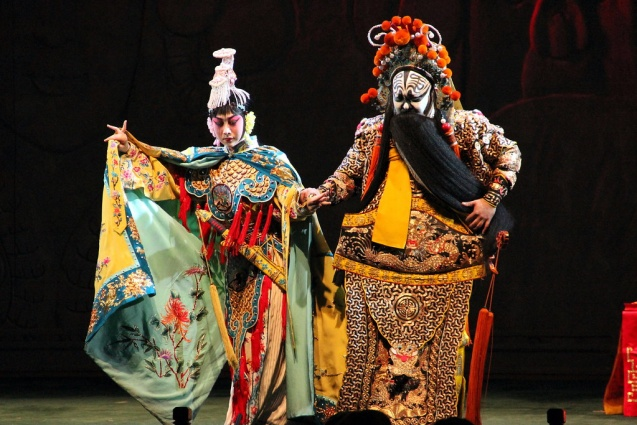
\includegraphics[width=1.16667in,height=0.96319in]{media/image16.jpeg} &
\reduline{\_\_8\_\_} &
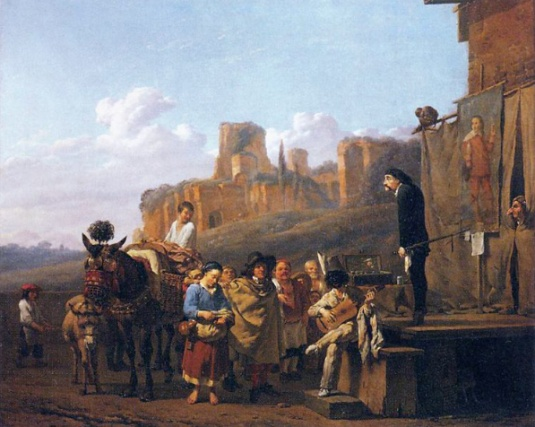
\includegraphics[width=1.16127in,height=0.95833in]{media/image17.jpeg}\tabularnewline
\reduline{\_\_2\_\_} &

\includegraphics[width=1.09375in,height=1.09375in]{media/image18.jpeg} &
\reduline{\_\_4\_\_} &
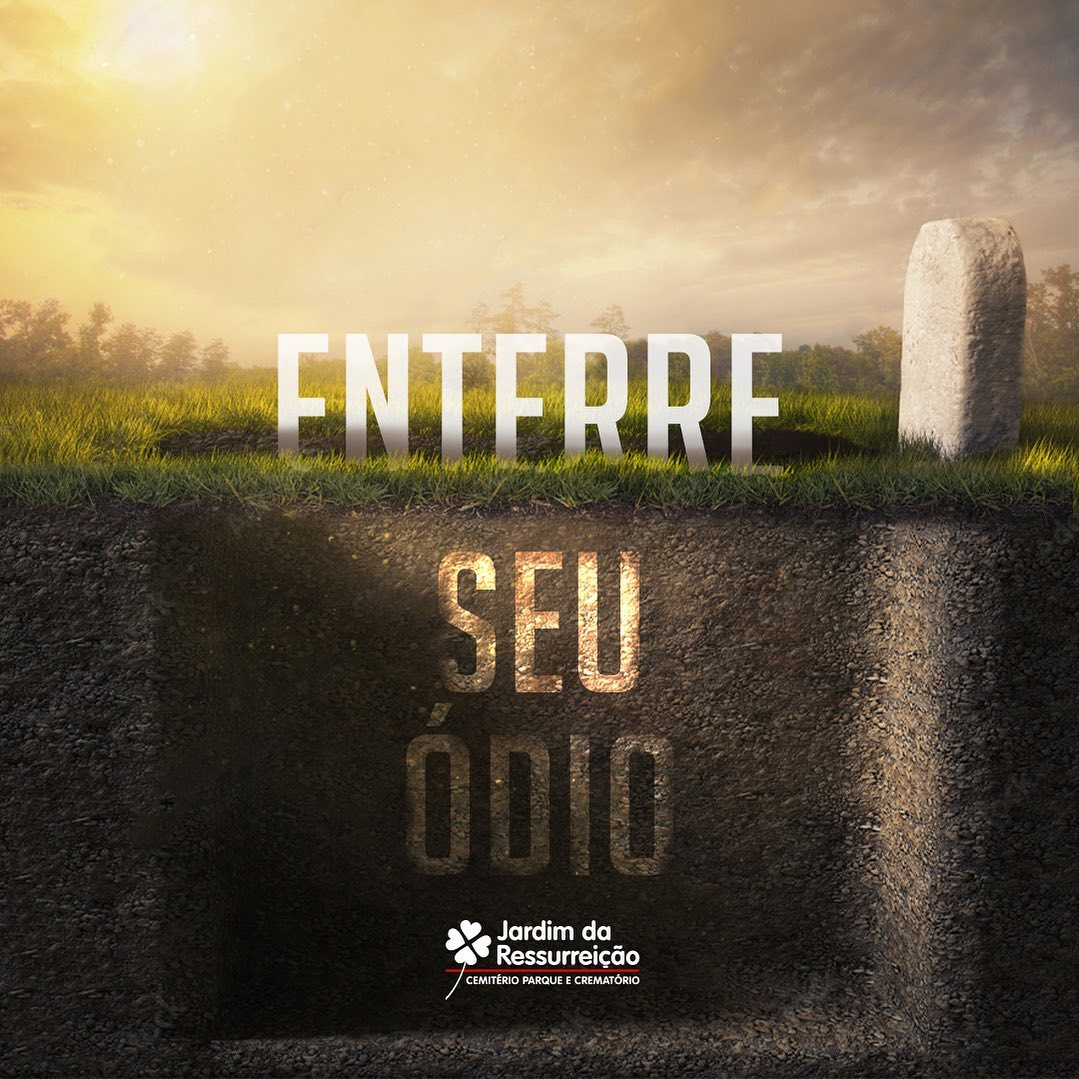
\includegraphics[width=1.27986in,height=0.98958in]{media/image19.jpeg}\tabularnewline
\reduline{\_\_3\_\_} &
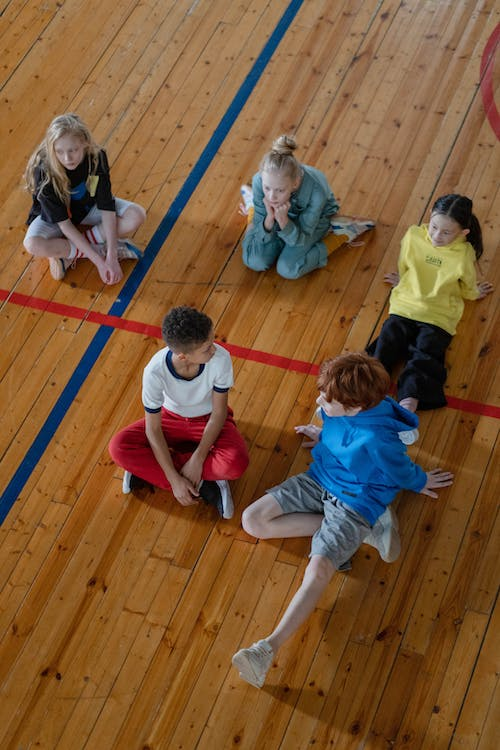
\includegraphics[width=0.92708in,height=0.92708in]{media/image20.jpeg} &
\reduline{\_\_6\_\_} &

\includegraphics[width=0.97986in,height=1.05208in]{media/image21.jpeg}\tabularnewline
\reduline{\_\_1\_\_} &
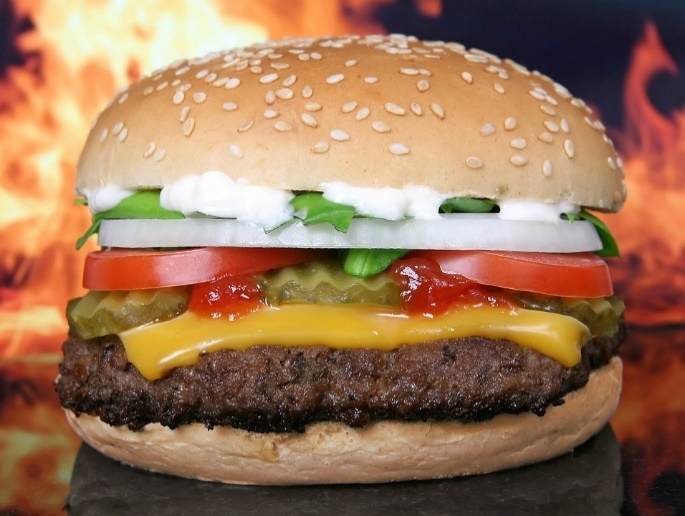
\includegraphics[width=1.13542in,height=1.13542in]{media/image22.jpeg} &
\reduline{\_\_7\_\_} &
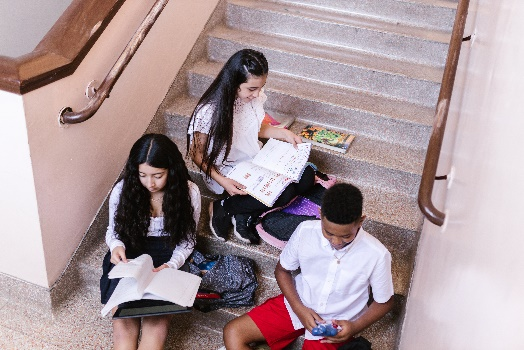
\includegraphics[width=1.23958in,height=1.15833in]{media/image23.jpeg}\tabularnewline
\reduline{\_\_9\_\_} &
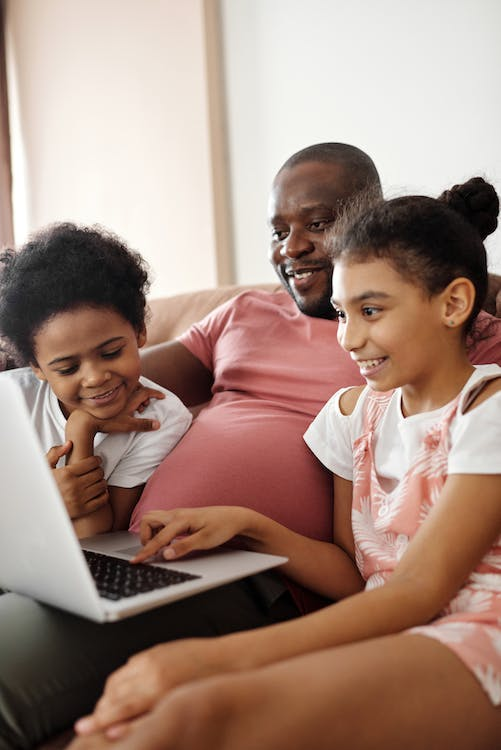
\includegraphics[width=1.19722in,height=1.27083in]{media/image24.jpeg} &
\reduline{\_\_5\_\_} &

\includegraphics[width=2.21875in,height=1.11458in]{media/image25.jpeg}\tabularnewline
\end{longtable}

\pagebreak
\num{7} Complete as palvaras com \textbf{-ca -co -cu} ou \textbf{-qua -que -qui}.

%\coment{Convide as crianças a falar o nome das imagens para identificar a grafia da palavra.}

\begin{figure}[htpb!]

\includegraphics[width=.24\textwidth]{media/image26.jpeg}
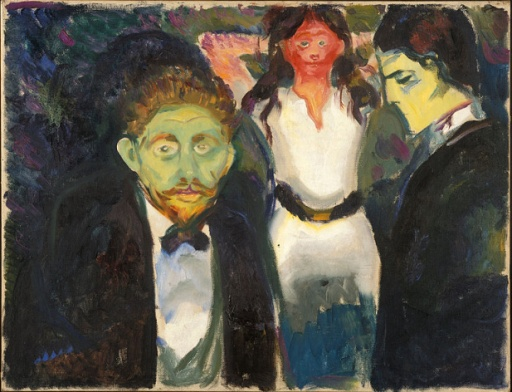
\includegraphics[width=.24\textwidth]{media/image27.jpeg}
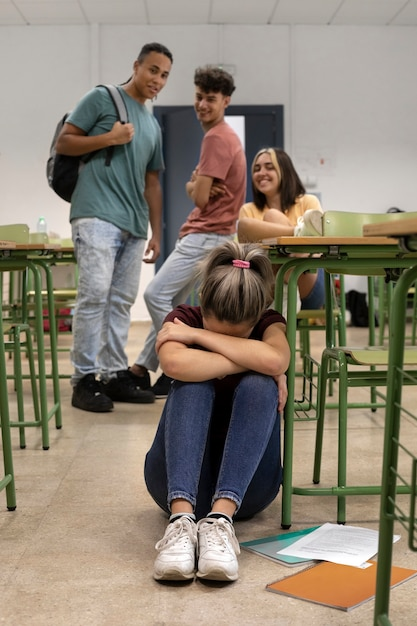
\includegraphics[width=.24\textwidth]{media/image28.jpeg}
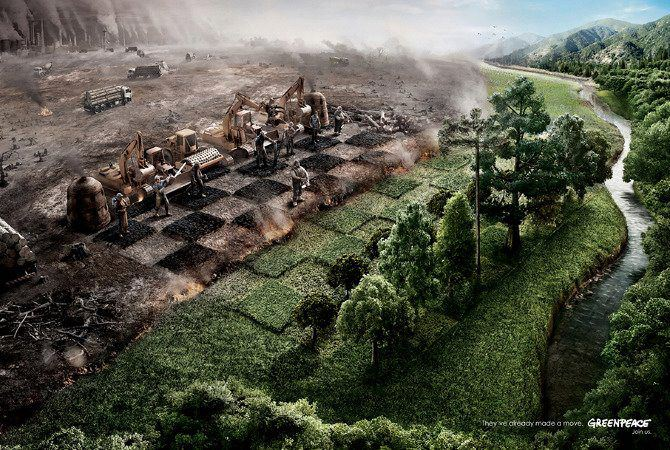
\includegraphics[width=.24\textwidth]{media/image29.jpeg}
\end{figure}

\reduline{CU} TIA \hspace{2cm} \reduline{CA} SA \hspace{2cm} \reduline{CU} SCUZ \hspace{2cm} \reduline{QUE} IJO

\begin{figure}[htpb!]
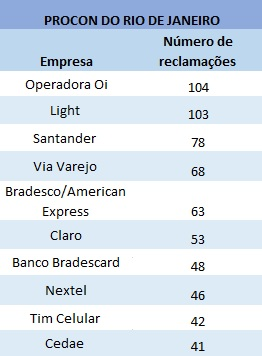
\includegraphics[width=.24\textwidth]{media/image30.jpeg}

\includegraphics[width=.24\textwidth]{media/image31.jpeg}
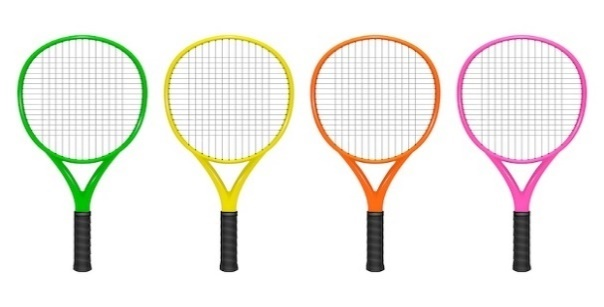
\includegraphics[width=.24\textwidth]{media/image32.jpeg}
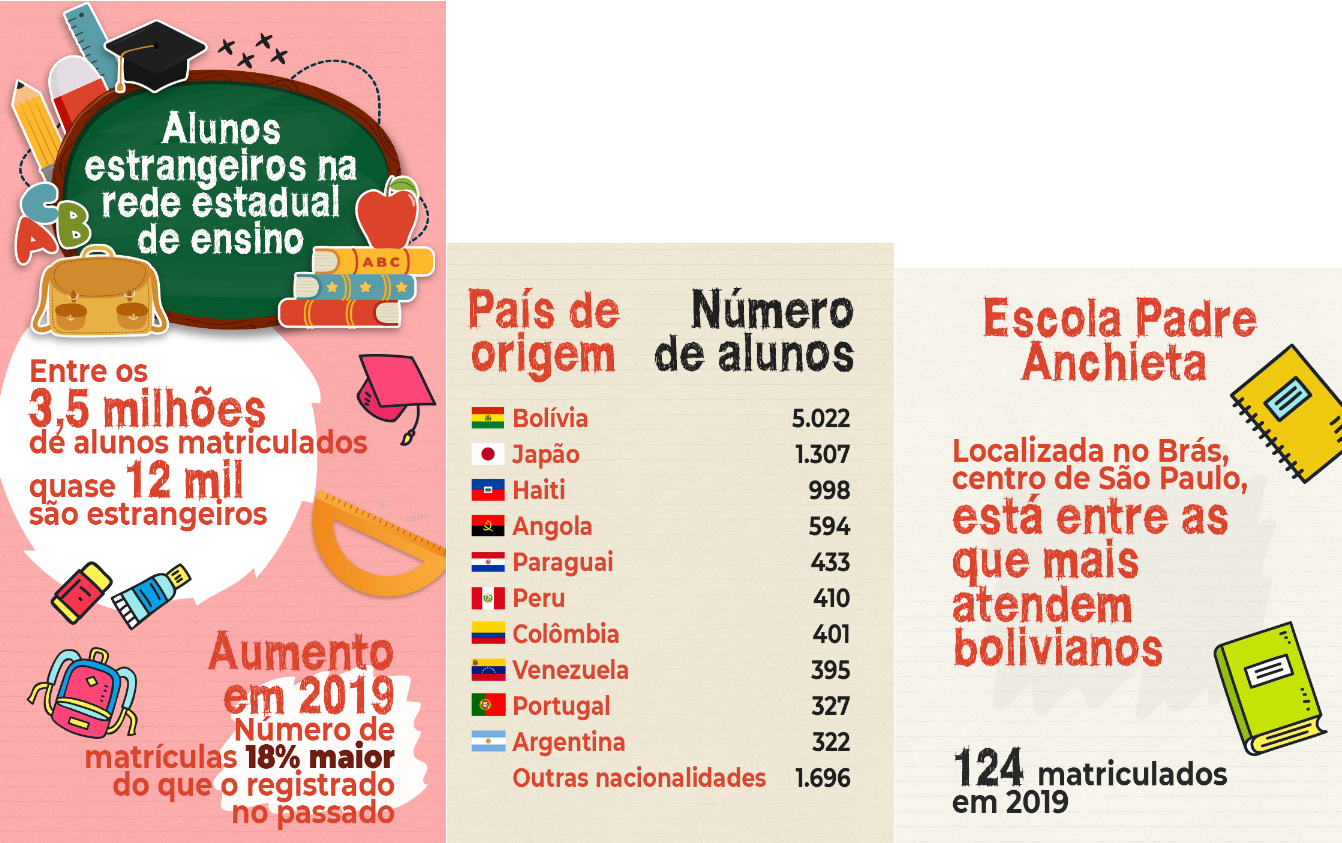
\includegraphics[width=.24\textwidth]{media/image33.jpeg}
\end{figure}

A \reduline{QUÁ} RIO \hspace{1cm} \reduline{QUI} NZE \hspace{1cm} RA \reduline{QUE} TE \hspace{1cm} \reduline{CO} LA


\num{8} Encontre a sílaba mais forte e complete com O ou U.

%\coment{Leve para a classe uma caixinha enfeitada com palavras terminadas com O e U. Passe a caixinha para os alunos em círculo, ao som de uma música. Quando a música parar, o aluno que estiver com a caixinha na mão deve ler a palavra observando a letra  final. Em seguida, convide toda a turma a pronunciar a palavra e, então, descobrir a sílaba forte. Explique como descobrir quando a sílaba é forte e fraca, ensinando que, quando o U está no final, ele é sempre forte, e que o O é sempre fraco no final das palavras.}

\begin{figure}[htpb!]

\includegraphics[width=.3\textwidth]{media/image34.jpeg}

\includegraphics[width=.3\textwidth]{media/image35.jpeg}
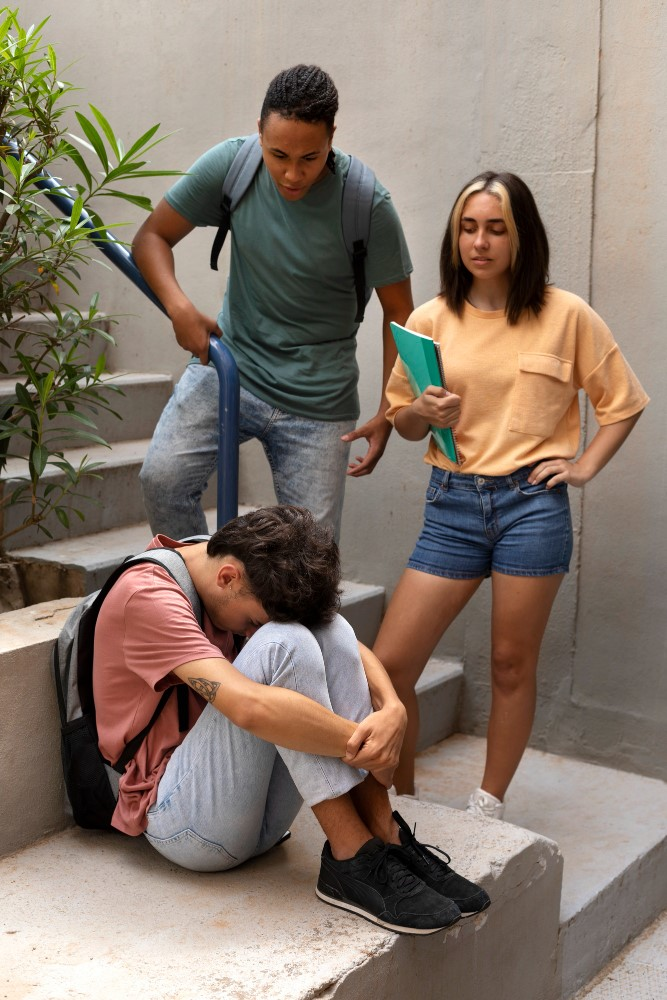
\includegraphics[width=.2\textwidth]{media/image36.jpeg}
\end{figure}

SAPAT \reduline{O} \hspace{3cm} VAS \reduline{O} \hspace{2cm} TAT \reduline{U}

\begin{figure}[htpb!]
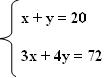
\includegraphics[width=.2\textwidth]{media/image37.jpeg}
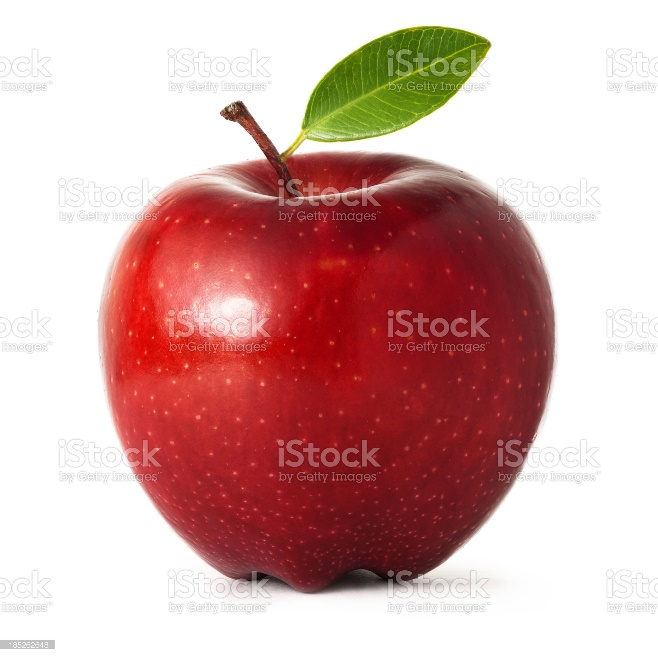
\includegraphics[width=.3\textwidth]{media/image38.jpeg}

\includegraphics[width=.2\textwidth]{media/image39.jpeg}
\end{figure}

ESPELH \reduline{O} \hspace{1cm} CAJ \reduline{U} \hspace{2cm} CABEL \reduline{O}


\num{9} Pinte as palvras escritas com C que tem o som de S.
%Felipe: aqui precisamos padronizar, como comentei anteriormente. 

%\coment{Leve para sala palavras escritas com C. Organize uma roda de conversa na qual você orientará os alunos a organizar as palavras de acordo com a vogal que acompanha a letra C. Em seguida, explique a regra para descobrir se o C tem som de K ou S.}

\begin{longtable}[]{@{}lllll@{}}
\toprule
\textbf{CINEMA} & \textbf{CASA} & \textbf{CISNE} & \textbf{CEGO} &
\textbf{COCADA}\tabularnewline
\midrule
\endhead
\textbf{CADEIRA} & \textbf{CARRO} & \textbf{CINTO } & \textbf{COCO} &
\textbf{CAMA}\tabularnewline
\bottomrule
\end{longtable}

\num{10} Troque as letras e forme outras palavras.

%\coment{Utilize o alfabeto móvel com as palavras solicitadas no exercício e outras. Também é possível fazer a brincadeira da forca.}

\begin{longtable}[]{@{}lll@{}}
\toprule
\textbf{V POR F} & \textbf{D POR T} & \textbf{B POR P}\tabularnewline
\midrule
\endhead
\textbf{VACA} & \textbf{DADO} & \textbf{BODE}\tabularnewline
\textbf{\reduline{F}ACA} & \textbf{\reduline{T}ATO} & \textbf{\reduline{P}ODE}\tabularnewline
\textbf{VILA} & \textbf{DIA} & \textbf{BOTE}\tabularnewline
\textbf{\reduline{F}I LA} & \textbf{\reduline{T}IA} & \textbf{\reduline{P}OTE}\tabularnewline
\bottomrule
\end{longtable}

\pagebreak
\num{11} Complete a cruzadinha com o nome das figuras.

%\coment{Explore as frutas e legumes da atividade, fazendo questionamentos. Monte as palavras no alfabeto móvel com as crianças. Em seguida, oriente a escrita na cruzadinha.}

\begin{figure}[htpb!]

\includegraphics[width=\textwidth]{media/image40.png}
\end{figure}

\num{12} Encontre e pinte as palavras no diagrama.

%\coment{Depois da leitura das palavras, oriente os alunos a localizá-las no diagrama.}

\begin{longtable}[]{@{}llllllll@{}}
\toprule
	TATU -- CABELO -- BONECA -- PANELA -- CAJU\tabularnewline
FADA -- DADO -- VASO -- CAMA -- TAPETE\tabularnewline
\midrule
D & B & F & A & D & A & D & G\tabularnewline
A & C & A & B & E & L & O & U\tabularnewline
G & Y & B & O & C & A & M & A\tabularnewline
S & T & I & N & H & M & A & Q\tabularnewline
P & A & N & E & L & A & D & F\tabularnewline
H & T & O & C & A & J & U & L\tabularnewline
J & U & K & A & D & A & D & O\tabularnewline
T & A & P & E & T & E & Z & X\tabularnewline
K & V & A & S & O & B & G & J\tabularnewline
\end{longtable}

\pagebreak
\colorsec{Treino}

\num{1} Observe o animal que Júlia encontrou enquanto brincava na 
fazenda do Tio Belo.

\begin{figure}[htpb!]
\centering

\includegraphics[width=.9\textwidth]{media/image42.jpeg}
\end{figure}

A palavra que começa com a mesma letra do nome do animal que Júlia encontrou é

\begin{escolha}
\item vaso.

\item gato.

\item bola.

\item foca
\end{escolha}


\num{2} Observe a palavra que Tiago leu para sua professora.

\begin{myquote}
CAJU
\end{myquote}

O nome da figura que termina com a mesma letra da palavra que Tiago leu é

\begin{escolha}
\item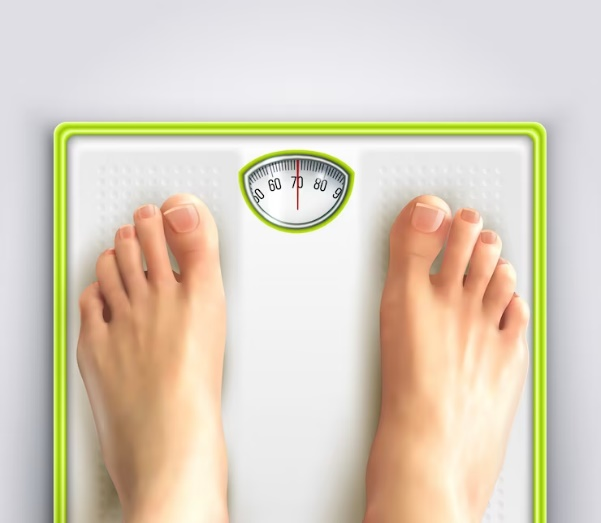
\includegraphics[width=0.79792in,height=0.81667in]{media/image44.jpeg}

\item
\includegraphics[width=1.02847in,height=0.72292in]{media/image45.jpeg}

\item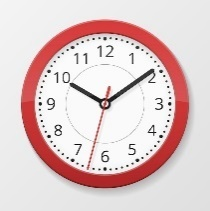
\includegraphics[width=0.79792in,height=0.79931in]{media/image46.jpeg}

\item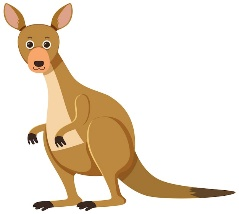
\includegraphics[width=1.08611in,height=0.97222in]{media/image47.jpeg}
\end{escolha}


\num{3} Observe o presente que Bruna ganhou.

\begin{figure}[htpb!]
\centering
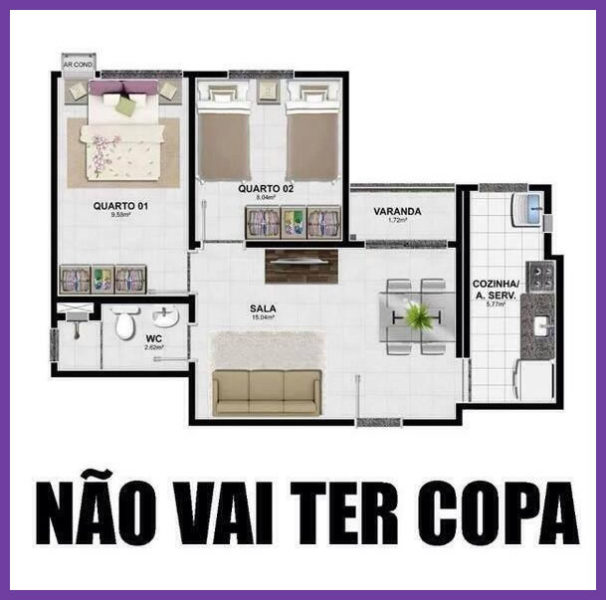
\includegraphics[width=.3\textwidth]{media/image48.jpeg}
\end{figure}

A palavra que começa como o mesmo som da letra do nome do presente de Bruna é

\begin{multicols}{2}
\begin{escolha}
\item cama.

\item cubo.

\item cebola.

\item cocada.
\end{escolha}
\end{multicols}

\chapter{Lendo e escrevendo}
\markboth{Módulo 2}{}

\vspace*{-1.5cm}

\colorsec{Habilidades do SAEB}

\begin{itemize}
\item Ler palavras.
\item Escrever palavras.
\item Ler frases.
\end{itemize}

\colorsec{Habilidades da BNCC}

\begin{itemize}
\item EF02LP04, EF02LP05.
\end{itemize}

\conteudo{Para escrever uma palavra, você precisa usar as letras que
são chamadas de vogais e as consoantes.

As vogais são 

\begin{myquote}
\textbf{A -- E -- I -- O -- U} 
\end{myquote}

e as consoantes são

\begin{myquote}
\textbf{B -- C -- D -- F -- G -- H -- J -- K -- L -- M -- N -- P -- Q -- R -- S
-- T -- V -- W -- Y -- X -- Z.}
\end{myquote}

As palavras são lidas e escritas da esquerda para a direita.

\begin{myquote}
$\longrightarrow$

\textbf{GRAVIOLA LÂMPADA AVIÃO LARANJA }
\end{myquote}

Existem diferentes maneiras de compor a sílaba de uma palavra. 

\textbf{CONSOANTE + VOGAL}: é o que acontece nas três sílabas das 
palavras \textit{sapato} e \textit{telefone}: SA-PA-TO e TE-LE-FO-NE

\textbf{VOGAL}: é o que acontece na segunda sílaba das  
palavras \textit{saída} e \textit{saúde}: SA-Í-DA e SA-Ú-DE

\textbf{CONSOANTE + VOGAL + CONSOANTE}: é o que acontece na 
primera sílaba das palavras \textit{porta} e \textit{cortina}:
POR-TA e COR-TI-NA

\textbf{CONSOANTE + CONSOANTE + VOGAL}: é o que acontece na 
primera sílaba da palavra \textit{criança} e na última
sílaba da palavra \textit{livro}: CRI-AN-ÇA e LI-VRO 

Observe o quadro abaixo, com outros exemplos:\bigskip

\noindent{\tiny
\begin{tabular}{l|l|l|l|l|}
\cline{2-5}
 & \textbf{GRAVIOLA} & \textbf{LÂMPADA} & \textbf{AVIÃO} & \textbf{LARANJA} \\ \hline
\multicolumn{1}{|l|}{\textbf{FORMAÇÃO SILÁBICA CV}} & GRA - \textbf{VI} - O - \textbf{LA} & LÂM - \textbf{PA} - \textbf{DA} & A - \textbf{VI} -ÃO & \textbf{LA} - RAN - \textbf{JA} \\ \hline
\multicolumn{1}{|l|}{\textbf{FORMAÇÃO SILÁBICA V}} & GRA - VI - \textbf{O} - LA & \multicolumn{1}{c|}{*} & \textbf{A} - VI -ÃO & \multicolumn{1}{c|}{*} \\ \hline
\multicolumn{1}{|l|}{\textbf{FORMAÇÃO SILÁBICA CVC}} & \multicolumn{1}{c|}{*} & \textbf{LÂM} - PA - DA & \multicolumn{1}{c|}{*} & LA - \textbf{RAN} - JA \\ \hline
\multicolumn{1}{|l|}{\textbf{FORMAÇÃO SILÁBICA CCV}} & \textbf{GRA} - VI - O - LA & \multicolumn{1}{c|}{*} & \multicolumn{1}{c|}{*} & \multicolumn{1}{c|}{*} \\ \hline
\end{tabular}
}


Note que, em todas as formações das sílabas, aparecem vogais. Isso
acontece porque não existe sílaba sem vogal, isto é, uma  sílaba não
se forma só com consoantes.

Observe a frase a seguir:

\begin{myquote}
\textbf{O avião pousou cedo.}
\end{myquote}

Você conhece esse sinal em cima da letra A da palavra \textbf{avião}?

Esse sinal é o \textbf{til}, usado nas vogais A e O para marcar a
nasalidade presente na sílaba.

As marcas de nasalidade aparece também nas letras M e N, no final da
sílaba. É o que acontece, por exemplo, com as seguintes palavras:

\begin{myquote}
\textbf{LÂMPADA E LARANJA}
\end{myquote}

A letra \textbf{M} é utilizada antes das consoantes P e B.  
A letra \textbf{N} é usada antes das demais consoantes, nunca 
no final das palavras.
}

\colorsec{Atividades}

\num{1} Escreva os nomes das figuras.

%\coment{Leve o alfabeto móvel para a sala de aula. Convide as crianças para manusear as letras; em seguida, oriente-as a formar as palavras que nomeiam as figuras. Sugira a elas que, antes de escrever, elas devem pronunciar a palavra, escrevendo-a por sílabas ou pedacinhos.}


\begin{figure}[htpb!]
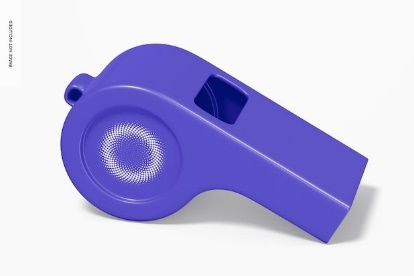
\includegraphics[width=1.46154in,height=0.93603in]{media/image49.jpeg}

\includegraphics[width=1.16587in,height=0.93269in]{media/image50.jpeg}
\includegraphics[width=1.42308in,height=1.21950in]{media/image51.jpeg}
\end{figure}

\reduline{Apito\hfill}

\reduline{Bicicleta\hfill}

\reduline{Árvore\hfill}

\begin{figure}[htpb!]
\includegraphics[width=1.10833in,height=1.00903in]{media/image52.jpeg}
\includegraphics[width=0.85556in,height=0.92222in]{media/image53.jpeg}
\includegraphics[width=0.79808in,height=0.79808in]{media/image54.jpeg}
\end{figure}

\reduline{Bola\hfill}

\reduline{Raposa\hfill}

\reduline{Gaiola\hfill}

\begin{figure}[htpb!]
\includegraphics[width=0.91319in,height=1.16319in]{media/image55.jpeg}
\includegraphics[width=1.62569in,height=1.25000in]{media/image56.jpeg}
\includegraphics[width=0.93990in,height=1.27885in]{media/image57.jpeg}
\end{figure}

\reduline{Pera\hfill}

\reduline{Pedra\hfill}

\reduline{Unha\hfill}

\pagebreak
\num{2} Separe as sílabas das palavras, depois circule as sílabas formadas por
consoante + consoante + vogal.

%\coment{Leia as palavras com os alunos, orientando-os a identificar vogais e consoantes. Também é possível montar algumas palavras com o alfabeto móvel. Em seguida, peça a eles que batam palmas cada vez que um pedacinho da palavra for pronunciado.}

\begin{longtable}[]{@{}ll@{}}
\toprule
\textbf{PRATO} & \rosa{Pra - to}\tabularnewline
\midrule
\textbf{FORMIGA} & \rosa{For- mi -ga}\tabularnewline
\midrule
\textbf{BRAÇO} & \rosa{Bra -ço}\tabularnewline
\midrule
\textbf{DRAGÃO} & \rosa{Dra- gão}\tabularnewline
\midrule
\textbf{CRAVO} & \rosa{Cra -- vo}\tabularnewline
\bottomrule
\end{longtable}

\num{3} Ligue as palavras com seu desenho.

%\coment{Leve para sala as palavras dentro de uma sacola. Cada criança deve pegar uma palavra da sacola para fazer a leitura. Depois proponha a atividade.}

Bicicleta \hfill\includegraphics[width=.1\textwidth]{media/image59.png}

Janela \hfill\includegraphics[width=.1\textwidth]{media/image60.png}

Borboleta \hfill\includegraphics[width=.1\textwidth]{media/image61.png}

Dragão \hfill\includegraphics[width=.1\textwidth]{media/image62.png}

Avião \hfill\includegraphics[width=.1\textwidth]{media/image63.png}

Prego \hfill\includegraphics[width=.1\textwidth]{media/image64.jpeg}

Pomba \hfill\includegraphics[width=.1\textwidth]{media/image65.png}

Manga \hfill\includegraphics[width=.1\textwidth]{media/image66.png}


\pagebreak
\num{4} Pinte no diagrama as palavras do quadro abaixo.

%\coment{Faça a leitura das palavras com os alunos aproveite esse momento para trabalhar a função da escrita.}

\begin{quote}\parindent=0em
\vspace*{-.5cm}
\begin{multicols}{3}
PIÃO

CAMA

LEÃO

PEDRA

ABACATE

SAPO

PATO

SABÃO

TRATOR

GRAMA

CISNE
\end{multicols}
\end{quote}

\begin{longtable}[]{@{}llllllllll@{}}
\toprule
P & I & Ã & O & D & O & W & E & I & S\tabularnewline
F & H & P & I & S & A & B & Ã & O & A\tabularnewline
S & J & L & S & J & U & Y & U & J & P\tabularnewline
L & O & A & B & A & C & A & T & E & O\tabularnewline
E & U & I & D & A & S & A & L & K & A\tabularnewline
à & A & B & G & C & A & Y & J & G & P\tabularnewline
O & S & A & P & A & T & O & P & R & E\tabularnewline
Z & D & R & F & D & M & E & C & A & D\tabularnewline
L & T & R & A & T & O & R & Q & M & R\tabularnewline
B & U & G & T & E & Y & E & & A & A\tabularnewline
A & C & I & S & N & E & O & P & U & O\tabularnewline
L & O & L & O & C & A & M & A & A & G\tabularnewline
\bottomrule
\end{longtable}

%\coment{R: pião -- cama -- leão- pedra- abacate- sapo- cama- pato -- sabão -- trator -- grama- cisne.}

\num{5} Coloque o til nas palavras sempre que necessário.

%\coment{Construa com os alunos critérios para identificar as marcas de nasalidade de uma palavra. Sugira que leiam as palavras em voz alta e posicionem os dedos indicador e polegar sobre o nariz ao pronunciar palavras com esses sons, para perceberem a diferença, por exemplo, entre a pronúncia de palavras como \textit{lá} e \textit{lã}, \textit{manha} e \textit{manhã}. Explique que o til acompanha apenas as vogais A e O.}

\begin{multicols}{3}
IRMAO

SALA

MAO

PATO

MAÇA

VILA

MOLA

MANHA

LA
\end{multicols}

\num{6} Observe a marca de nasalização e complete as palavras com M ou N.

%\coment{Siga as orientações da questão anterior, aguçando a atenção das crianças quanto à diferença de pronúncia de palavras como \textit{pote} e \textit{ponte} e \textit{rapa} e \textit{rampa}. Reforce a ideia de M sempre antes de B, e N antes de outras consoantes.}

\begin{multicols}{3}
LÂ\reduline{M}PADA

CA\reduline{M}PO

LARA\reduline{N}JA

TRO\reduline{N}CO

VE\reduline{N}TO

PO\reduline{M}BA

U\reduline{M}BIGO

PO\reduline{N}TE

RA\reduline{M}PA

BO\reduline{M}BOM

TE\reduline{M}PO

PI\reduline{N}TA
\end{multicols}

\num{7} Observe as imagens e escreva uma frase para cada uma.

%\coment{Explore as imagens com as crianças e oriente a construção das frases.}

\begin{figure}[htpb!]
\centering
\includegraphics[width=.5\textwidth]{media/image67.jpeg}
\end{figure}

\reduline{Uma resposta possível é \textit{As crianças andam a cavalo}.\hfill}
\linhas{1}

\begin{figure}[htpb!]
\centering
\includegraphics[width=.5\textwidth]{media/image68.jpeg}
\end{figure}

\reduline{Uma resposta possível é \textit{A menina leva flores no carrinho}.\hfill}
\linhas{1}

\pagebreak
\num{8} Leia as frases a seguir e faça um desenho para representar.

%\coment{Oriente a leitura das frases explorando com as crianças o conteúdo de cada uma delas e as diferentes possibilidades de representação.}

\begin{myquote}
O CAVALO GOSTA DE CORRER.
\end{myquote}

\begin{mdframed}[linewidth=2pt,linecolor=salmao]
\vspace{7cm}
\end{mdframed}

\begin{myquote}
O MENINO JOGA BOLA.
\end{myquote}

\begin{mdframed}[linewidth=2pt,linecolor=salmao]
\vspace{7cm}
\end{mdframed}

\begin{myquote}
O PÁSSARO CANTA FELIZ.
\end{myquote}

\begin{mdframed}[linewidth=2pt,linecolor=salmao]
\vspace{7cm}
\end{mdframed}

\begin{myquote}
A ÁRVORE CAIU.
\end{myquote}

\begin{mdframed}[linewidth=2pt,linecolor=salmao]
\vspace{7cm}
\end{mdframed}

%\coment{Respostas pessoais dos alunos.}

\num{9} Forme palavras de acordo com a numeração, depois forme uma frase.

%\coment{Oriente os alunos a formar as palavras. Em seguida, trabalhe a função social de cada palavra para facilitar a construção das frases.}

\begin{longtable}[]{@{}lllll@{}}
\toprule
\begin{minipage}[b]{0.19\columnwidth}\raggedright\strut
1

BO\strut
\end{minipage} & \begin{minipage}[b]{0.19\columnwidth}\raggedright\strut
2

PI\strut
\end{minipage} & \begin{minipage}[b]{0.19\columnwidth}\raggedright\strut
3

NE\strut
\end{minipage} & \begin{minipage}[b]{0.19\columnwidth}\raggedright\strut
4

CO\strut
\end{minipage} & \begin{minipage}[b]{0.19\columnwidth}\raggedright\strut
5

ÃO\strut
\end{minipage}\tabularnewline
\midrule
\endhead
\begin{minipage}[t]{0.19\columnwidth}\raggedright\strut
6

CAM\strut
\end{minipage} & \begin{minipage}[t]{0.19\columnwidth}\raggedright\strut
7

BRA\strut
\end{minipage} & \begin{minipage}[t]{0.19\columnwidth}\raggedright\strut
8

CIS\strut
\end{minipage} & \begin{minipage}[t]{0.19\columnwidth}\raggedright\strut
9

CA\strut
\end{minipage} & \begin{minipage}[t]{0.19\columnwidth}\raggedright\strut
10

ÇO\strut
\end{minipage}\tabularnewline
\midrule
\begin{minipage}[t]{0.19\columnwidth}\raggedright\strut
11

MA\strut
\end{minipage} & \begin{minipage}[t]{0.19\columnwidth}\raggedright\strut
12

JA\strut
\end{minipage} & \begin{minipage}[t]{0.19\columnwidth}\raggedright\strut
13

LA\strut
\end{minipage} & \begin{minipage}[t]{0.19\columnwidth}\raggedright\strut
14

CA\strut
\end{minipage} & \begin{minipage}[t]{0.19\columnwidth}\raggedright\strut
15

PO\strut
\end{minipage}\tabularnewline
\bottomrule
\end{longtable}

\textbf{PALAVRA FRASE}

\begin{itemize}
\item 1 + 3 + 14 \reduline{\mbox{ }\hfill}

\item 7 + 10 \reduline{\mbox{ }\hfill}

\item 2 + 5 \reduline{\mbox{ }\hfill}

\item 6 + 15 \reduline{\mbox{ }\hfill}

\item 8 + 3 \reduline{\mbox{ }\hfill}

\item 12 + 3 + 13 \reduline{\mbox{ }\hfill}

\item 11 + 9 + 4 \reduline{\mbox{ }\hfill}
\end{itemize}

\num{10} Complete os nomes das frutas com as vogais corretas.

%\coment{Reapresente as vogais aos alunos de acordo com as palavras do exercício. Forme as palavras ressaltado sempre que não existe sílaba sem vogal.}

\begin{figure}[htpb!]
\includegraphics[width=.24\textwidth]{media/image69.jpeg}
\includegraphics[width=.24\textwidth]{media/image70.jpeg}
\includegraphics[width=.24\textwidth]{media/image71.jpeg}
\includegraphics[width=.24\textwidth]{media/image72.jpeg}
\end{figure}

\reduline{U}V\reduline{A} \hspace{1.5cm} L\reduline{A}R\reduline{A}NJ\reduline{A} \hspace{1cm} \reduline{A}B\reduline{A}C\reduline{A}X\reduline{I} \hspace{1cm} B\reduline{A}N\reduline{A}N\reduline{A}

\begin{figure}[htpb!]
\includegraphics[width=.24\textwidth]{media/image73.jpeg}
\includegraphics[width=.24\textwidth]{media/image74.jpeg}
\includegraphics[width=.24\textwidth]{media/image75.jpeg}
\includegraphics[width=.24\textwidth]{media/image76.jpeg}
\end{figure}

P\reduline{Ê}R\reduline{A} \hspace{1cm} M\reduline{O}R\reduline{A}NG\reduline{O} \hspace{1cm} G\reduline{O}\reduline{I}\reduline{A}B\reduline{A} \hspace{1cm} M\reduline{A}Ç\reduline{Ã}

\num{11} Organize as palavras de acordo com sua formação silábica.

%\coment{Leve o alfabeto para sala. Explore as vogais e as consoantes com os alunos. Realize com eles a formação de algumas palavras, identificado as diferentes formações silábicas. Brincar de \textbf{forca} é uma boa opção para desenvolver essa atividade.}

\begin{myquote}
ABACAXI -- TRATOR - GRAVIOLA - PRATO -- CAMPO - CISNE - BAÚ
\end{myquote}

{\small
\begin{tabular}{|l|l|l|l|}
\hline
\textbf{\begin{tabular}[c]{@{}l@{}}PALAVRAS COM\\ FORMAÇÃO CV\end{tabular}} & \textbf{\begin{tabular}[c]{@{}l@{}}PALAVRAS COM\\ FORMAÇÃO V\end{tabular}} & \textbf{\begin{tabular}[c]{@{}l@{}}PALAVRAS COM\\ FORMAÇÃO CCV\end{tabular}} & \textbf{\begin{tabular}[c]{@{}l@{}}PALAVRAS COM\\ FORMAÇÃO CVC\end{tabular}} \\ \hline
\rosa{ABACAXI} & \rosa{GRAVIOLA} & \rosa{TRATOR} & \rosa{CISNE} \\ \hline
\rosa{GRAVIOLA} & \rosa{ABACAXI} & \rosa{GRAVIOLA} & \rosa{CAMPO} \\ \hline
\rosa{PRATO} & \rosa{BAÚ} & \rosa{PRATO} &  \\ \hline
\rosa{CAMPO} &  &  &  \\ \hline
\rosa{CISNE} &  &  &  \\ \hline
\rosa{BAÚ} &  &  &  \\ \hline
\end{tabular}
}

\pagebreak
\colorsec{Treino}

\num{1} Mila foi à feira e comprou seu brinquedo preferido com as
econonias de seu cofrinho.

\begin{figure}[htpb!]
\centering
\includegraphics[width=.5\textwidth]{media/image77.jpeg}
\end{figure}

Qual palavra tem a primeira sílaba com a mesma formação da primeira
sílaba do nome do brinquedo de Mila?

\begin{multicols}{2}
\begin{escolha}
\item abacate.

\item janela.

\item traça.

\item prego.
\end{escolha}
\end{multicols}

\num{2} Leia a frase.

\begin{myquote}
\textbf{A menina brinca com bolhas de sabão.}
\end{myquote}

A imagem que representa o que está escrito na frase é

\begin{multicols}{2}
\begin{escolha}
\item\includegraphics[width=0.75159in,height=1.04531in]{media/image78.jpeg}

\item\includegraphics[width=1.23681in,height=1.10139in]{media/image79.jpeg}

\item\includegraphics[width=0.97361in,height=1.05069in]{media/image80.jpeg}

\item\includegraphics[width=0.75437in,height=1.04404in]{media/image81.jpeg}
\end{escolha}
\end{multicols}


\num{3} Veja a palavra nova que Ana aprendeu a ler.

\begin{myquote}
FORMIGA
\end{myquote}

A primeira sílaba da palavra acima tem a mesma formação que a 
primeira sílaba de

\begin{escolha}
\item borboleta.

\item dragão.

\item laranja.

\item garota.
\end{escolha}


\chapter[Encontrando informações no texto]{\Large Encontrando informações no texto}
\markboth{Módulo 3}{}

%Para iniciar este módulo, é possível comentar os tipos dos textos que serão lidos e explorar bastante a oralidade, fazendo diversos questionamentos de informações que estão nos textos.

\colorsec{Habilidade do SAEB}

\begin{itemize}
	\item Localizar informações explícitas em textos
\end{itemize}

\colorsec{Habilidades da BNCC}

\begin{itemize}
\item EF15LP03
\end{itemize}

\conteudo{

\begin{verse}
\textbf{Meu galinho}

Há três noites que eu não durmo\\
Ó lá lá\\
Pois perdi o meu galinho\\
O lá lá\\
Coitadinho o lá lá,\\
Pobrezinho o lá lá\\
Se perdeu lá no jardim.

Ele é branco e amarelo\\
O lá lá\\
Tem a crista vermelhinha\\
O lá lá\\
Bate as asas, o lá lá,\\
Abre o bico o lá lá\\
E faz qui qui ri qui qui
\end{verse}

\fonte{Disponível em: http://www.dominiopublico.gov.br/download/texto/me000588.pdf. Acesso em: 19 abr. 2023. }

Por que ele não dorme?

Onde o galo se perdeu?

Quais são as cores do galo?

Para responder a essas e outras perguntas, você precisa buscar as
informações no texto. Elas estão todas lá, de forma bem clara. 
Basta observar com atenção.

Observe o seguinte cartaz:\bigskip

\noindent\includegraphics[width=\textwidth]{media/image82.png}\bigskip

Está bem claro que esse cartaz contém um pedido de doação de brinquedos.
}

\colorsec{Atividades}

\num{1} Vamos cantar.

%\coment{Convide as crianças para brincar com a música, usando o nome dos alunos da turma. Em seguida faça questionamentos sobre a música: onde a canoa virou? Maria estava sozinha? Alguém socorreu Maria?}

\begin{quote}
\begin{verse}
\textbf{A canoa virou}

A canoa virou,\\
pois deixaram virar.\\
Foi por causa da maria,\\
que não soube remar.

Se eu fosse um peixinho\\
e soubesse nadar,\\
eu tirava a maria\\
do fundo do mar.
\end{verse}

\fonte{Política Nacional de Alfabetização. Cantigas. Disponível em: https://tinyurl.com/yckw7p6b. Acesso em: 19 abr. 2023. }
\end{quote}

\begin{escolha}
\item Escreva o título da música.

\reduline{A canoa virou.\hfill}
\linhas{1}

\item Por que a canoa virou?

\reduline{Maria não soube remar.\hfill}
\linhas{1}

\item Se eu fosse um peixinho o que eu faria?

\reduline{Se eu fosse um peixinho, eu tirava Maria do fundo do mar.\hfill}
\linhas{1}
\end{escolha}

\num{2} Vamos brincar de trem?

%\coment{Convide os alunos para formar um trem. Nesse momento, podem ser trabalhadas as noções de \textbf{lateralidade}: frente, trás, entre. Faça os questionamentos orais para trabalhar a fala e a escuta com as crianças.}

\begin{quote}
\begin{verse}
\textbf{O trem maluco}

O trem maluco,\\
quando sai de Pernambuco,\\
vai fazendo xique-xique\\
até chegar ao Ceará.
\end{verse}
\end{quote}

\begin{escolha}
\item  Encontre e circule o título da música.

\item De onde o trem sai?

\reduline{O trem sai de Pernambuco.\hfill}

\item Para onde o trem vai?

\reduline{O trem vai para o Ceará.\hfill}
\end{escolha}

\num{3} Vamos ler a letra da canção.\enlargethispage{2\baselineskip}

%\coment{Inicialmente, faça a leitura da letra da canção. Em seguida, convide as crianças a cantar. Depois, faça perguntas sobre o conteúdo da letra para trabalhar a oralidade.}

\begin{quote}
\begin{verse}
\textbf{Borboletinha}

Borboletinha\\
está na cozinha\\
fazendo chocolate\\
para a madrinha\\
poti,poti\\
perna de pau\\
olho de vidro\\
e nariz de pica-pau\\
tchau, tchau
\end{verse}

\fonte{Secretaria de Educação da Prefeitura de Diadema. Borboletinha. Disponível em: https://tinyurl.com/3n5ym7w5. Acesso em: 19 abr. 2023. }
\end{quote}

\begin{escolha}
\item Encontre e pinte de azul o nome da música.

\item Onde a borboletinha está?

\reduline{A borboletinha está na cozinha.\hfill}

\item O que ela está fazendo?

\reduline{A borboletinha está fazendo chocolate.\hfill}

\item Para quem é o cochocolate que ela está fazendo?

\reduline{A borboletinha está fazendo chocolate para a madrinha.\hfill}
\end{escolha}

\num{4} Observe esse cartaz.

%\coment{Pergunte as crianças o que elas vem no cartaz. Questione se já participaram de alguma campanha ou se já doaram roupas para outras pessoas. Aproveite e fale da importância de ser solidário.}

\begin{figure}[htpb!]
\centering
\includegraphics[width=.5\textwidth]{media/image83.jpeg}
\end{figure}
%\textbf{\url{http://www.saosebastiao.sp.gov.br/noticia.asp?id=N1122020143810.Acesso} 02 mar. 2023}

\begin{escolha}
\item Qual é a campanha mostrada no cartaz?

\reduline{O cartaz apresenta uma campanha de arrecadação de roupas.\hfill}

\item As roupas devem ser doadas a crianças de que idade?

\reduline{As roupas devem ser doadas a crianças de zero a 3 anos.\hfill}
\end{escolha}

\num{5} Vamos ler com atenção.

%\coment{Leia a receita para as crianças. Depois, pergunte a elas se conhecem esse tipo de texto. Identifique com elas as instruções apresentadas. A seguir, explore o conteúdo da receita, perguntando aos alunos, por exemplo, se conhecem os ingredientes e gostam deles.}

%Paulo: acredito que seria interessante colocar a receita abaixo em um box que lembrasse uma folha de papel, pautada ou não, se possível com uma fonte que lembre letra cursiva. 
\begin{quote}
\textbf{Macarrão de panela de pressão}

\textbf{Ingredientes}

%\includegraphics[width=1.94097in,height=1.14722in]{media/image84.jpeg}1

\begin{itemize}
\item 1 pacote de macarrão tipo parafuso

\item 1 saquinho molho de tomate

\item 1 caixa de creme de leite

\item Sal a gosto

\item Alho e cebola a gosto

\item 2 medidas do recipiente do molho de tomate de água

\end{itemize}

\textbf{Modo de fazer}

Em uma panela de pressão, frite o alho e a cebola. Depois, jogue o
macarrão e o molho de tomate e misture tudo. Aproveite o recipiente
do molho de tomate (o saquinho ou o pote): encha-o com água duas vezes
e jogue-a na panela.

Depois feche a panela e coloque no fogo. Assim que a panela pegar a
pressão, desligue, mas não abra e nem tire o pino: espere sair toda 
a pressão sozinha, lentamente. Quando isso acontecer, abra, mexa o
macarrão e coloque a caixa de creme de leite. Tempere com o sal a gosto.
Pronto! É só comer. 
\end{quote}

%Felipe ou Fábia: alterei esta receita (mandei mensagem no Odoo). Por isso, o link a seguir não é mais necessário: http://educacao.diadema.sp.gov.br/educacao/attachments/article/749/atividade\%209\%20semana\%20fase\%20I\%20Drummond.pdf.Acesso} 02 mar. 2023.
%https://www.freepik.com/premium-photo/spaghetti-dish-white-background\_4396472.htm\#query=MACARR\%C3\%83O\&position=8\&from\_view=search\&track=sph

\begin{escolha}
\item Qual é o nome do prato explicado na receita?

\reduline{O nome do prato explicado na receita é macarrão de panela de pressão.\hfill}

\item Encontre no texto e pinte de verde o nome do utensílio usado para
conzinhar o macarrão.

\reduline{O aluno deve pintar de verde a expressão ``panela de pressão''.\hfill}

\pagebreak
\item Agora escreva o nome de três ingredientes usados para fazer a receita.

\reduline{Os ingredientes usados para fazer a receita são macarrão, molho, creme de leite, sal, alho, cebola e água. O aluno deve escolher três deles.\hfill}
\end{escolha}

\num{6} Vamos cantar.

\begin{quote}
\begin{verse}
\textbf{Meu chapéu}

O meu chapéu tem três pontas,\\
tem três pontas o meu chapéu.\\
Se não tivesse três pontas,\\
não seria o meu chapéu.
\end{verse}

\fonte{Secretaria de Educação da Prefeitura de Diadema. Borboletinha. Disponível em: http://educacao.diadema.sp.gov.br/educacao/attachments/article/749/atividade\%209\%20semana\%20fase\%20I\%20Drummond.pdf. Acesso em: 19 abr. 2023. }
\end{quote}

\begin{escolha}
\item Quantas pontas tem o chapéu que aparece na canção?

\reduline{O chapéu descrito na letra da canção tem três pontas.\hfill}

\item Como você imagina que é esse chapéu? Desenhe.

\begin{mdframed}[linewidth=2pt,linecolor=salmao,roundcorner=10pt]
\coment{Resposta pessoal.}
\vspace{4cm}
\end{mdframed}
\end{escolha}

\num{7} Leia as informações do cartaz.

%\coment{Explore as informações do cartaz: a campanha de vacinação, o período em que acontece e a faixa etária a que se destina. Pergunte aos alunos se eles entendem o que significa a gotinha branca e peça-lhes que expliquem.}

\begin{figure}[htpb!]
\centering
\includegraphics[width=.5\textwidth]{media/image85.jpeg}
\end{figure}

%\url{https://barreiras.ba.gov.br/segunda-etapa-da-campanha-de-vacinacao-contra-o-sarampo-comeca-na-quinta-feira-14-em-barreiras/} Acesso 02 mar. 2023.

\begin{escolha}
\item Qual é a campanha divulgada no cartaz?

\reduline{A campanha divulgada no cartaz é a de vacinação contra o sarampo.\hfill}

\item Para quem é indicada essa vacinação?

\reduline{A vacinação é indicada para jovens e adultos de 20 a 29 anos.\hfill}

\item Em que período vai acontecer a campanha?
	
\reduline{A campanha vai acontecer de 18 a 30 de Novembro.\hfill}
\end{escolha}

\num{8} Leia o texto.

%\coment{Depois de cantar a canção e ler a letra, é interessante fazer uma dobradura do chapéu.}

\begin{quote}
\begin{verse}
\textbf{Marcha soldado}

Marcha soldado,\\
cabeça de papel.\\
Se não marchar direito,\\
vai preso pro quartel.

O quartel pegou fogo,\\
a polícia deu sinal.\\
Acode, acode, acode,\\
a bandeira nacional.
\end{verse}

\fonte{Política Nacional de Alfabetização. Cantigas. Disponível em: https://alfabetizacao.mec.gov.br/images/conta-pra-mim/livros/versao\_digital/cantigas\_versao\_digital.pdf. Acesso em: 19 abr. 2023. }
\end{quote}

\begin{escolha}
\item Localize no texto e pinte de vermelho como é a cabeça do soldado.

\item O que acontece com o soldado se não marchar direto?

\reduline{Se não marchar direito, o soldado vai preso.\hfill}

\end{escolha}

\num{9} Vamos cantar.

\begin{quote}
\begin{verse}
\textbf{Dona aranha}

A Dona Aranha subiu pela parede\\
veio a chuva forte e a derrubou\\
já passou a chuva\\
o sol já vai surgindo\\
e a Dona Aranha continua a subir
\end{verse}

\fonte{https://www2.bauru.sp.gov.br/arquivos/arquivos\_site/sec\_educacao/atividades\_pedagogica\_distancia/1;Infantil/49;EMEI\%20Maria\%20Elizabet\%20Camilo\%20de\%20P\%C3\%A1dua/5;PROF.\%C2\%AA\%20REBECA/Atividades\%20de\%2012\%20a\%2016\%20de\%20abril\_Infantil\%20II\%20B\_Prof\%C2\%AA\%20Rebeca.pdf.
Acesso 11 mar. 2023.}
\end{quote}

\begin{escolha}
\item Escreva o nome do animal que aparece na música.

\reduline{Aranha\hfill}

\pagebreak
\item Quem derrubou a Dona Aranha?

\reduline{A Dona Aranha foi derrubada pela chuva forte.\hfill}

\end{escolha}

\num{10} Vamos cantar.

\begin{quote}
\begin{verse}
\textbf{Pai Francisco}

Pai Francisco entrou na roda\\
tocando seu violão\\
vem de lá Seu Delegado\\
e Pai Francisco foi pra prisão.
\end{verse}
\end{quote}

%Tentei de todas as formas acessar a página a seguir, mas não consegui de jeito nenhum. Deve ser conteúdo restrito {http://servicos.rolandia.pr.gov.br/educacao/wp-content/uploads/aulas_online/cmeis/JOSEMARIA\%20ESCRIV\%C3\%81/INFANTIL-1/2021/16\%C2\%BAROT-I1B.pdf}Acesso 11 mar. 2023.

\begin{escolha}
\item Qual é o nome da canção?

\reduline{O nome da canção é ``Pai Francisco''.\hfill}

\item Desenhe o instrumento musical que Pai Francisco estava tocando.

\begin{mdframed}[linewidth=2pt,linecolor=salmao,roundcorner=10pt]
\vspace{8cm}
\end{mdframed}
\end{escolha}

\colorsec{Treino}

\num{1}

\begin{quote}
\begin{verse}
\textbf{Pintinho}

Meu pintinho amarelinho\\
cata aqui na minha mão,\\ 
na minha mão.\\
Quando quer comer bichinho,\\ 
com seu pezinho\\ 
ele cisca o chão.

Ele bate as asas,\\
ele faz piu-piu,\\ 
mas tem muito medo do gavião.
\end{verse}

\fonte{Domínio Público. Pintinho. Disponível em:
http://www.dominiopublico.gov.br/download/texto/me000588.pdf.
Acesso em: 19 abr. 2023.}
\end{quote}

O que o pintinho faz quando quer comer bichinho?

\begin{escolha}
	\item Cisca o chão.

	\item Bate as asas.

	\item Cata na mão.

	\item Faz piu-piu.
\end{escolha}

\pagebreak
\num{2} Leia o texto a seguir.

\begin{quote}
\begin{verse}
\textbf{Pombinha branca}

Pombinha branca \\
O que está fazendo?\\
Lavando a roupa\\
Do casamento.

A roupa é suja\\
É cor-de-rosa\\
Pombinha branca\\
É preguiçosa.

\end{verse}

\fonte{Domínio Público. Pombinha branca. Disponível em: http://www.dominiopublico.gov.br/download/texto/me000588.pdf. Acesso em: 19 abr. 2023.  }
\end{quote}

A pombinha é considerada preguiçosa porque

\begin{escolha}
	\item vai casar.

	\item a roupa está suja.

	\item só tem roupas cor-de-rosa.

	\item porque está lavando roupa.
\end{escolha}

\pagebreak
\num{3} Leia o texto.

\begin{quote}
\begin{verse}
\textbf{O tubo de cola}

O tubo de cola saiu da gaveta\\
caiu no tapete da sala.\\
a bola pulou no tapete melado e ficou colada na cola.\\
aí, a bola falou:\\
--- sapato, me ajuda!\\
o sapato ajudou.\\
deu um peteleco na bola\\
a bola melada colou no sapato.
\end{verse}

%Aqui temos um problema: o texto usado não está em área aberta do site. Não me preocupei com a diagramação do texto acima e da questão em geral.  

\fonte{https://portal.educacao.go.gov.br/wp-content/uploads/2021/04/Atividade-7-2o-ano-LP-LOCALIZAR-INFORMACOES-EXPLICITAS-EM-TEXTOS-E-EM-IMAGENS-GENERO-CONTOS.pd}
\end{quote}

De onde saiu o tubo da cola?

\begin{escolha}
\item DA BOLA

\item DO TAPETE.

\item DO SAPATO.

\item DA GAVETA.
\end{escolha}

\chapter{Para que serve este texto?}
\markboth{Módulo 4}{}

%Para iniciar o módulo, apresente os textos aos alunos pergunte se eles conhecem algum deles. Em seguida, explique a função de cada texto e a quem ele se destina.

\colorsec{Habilidade do SAEB}

\begin{itemize}
\item Reconhecer a finalidade de um texto.
\end{itemize}

\colorsec{Habilidade da BNCC}

\begin{itemize}
\item EF15LP01.
\end{itemize}

\conteudo{Você sabe para que servem os textos?

Existem vários tipos de textos, com linguagem e estrutura próprias e com 
diferentes funções.

Veja alguns deles e suas funções.

\includegraphics[width=.5\textwidth]{media/image86.jpeg}
\includegraphics[width=.5\textwidth]{media/image87.png}

\includegraphics[width=.5\textwidth]{media/image90.jpeg}
\includegraphics[width=.5\textwidth]{media/image92.png}
%\includegraphics[width=1.97452in,height=2.09063in]{media/image91.png}
}

%\textbf{https://www.flickr.com/photos/cbnsp/8264557482/in/photostream/}
%\textbf{https://agenciadenoticias.uniceub.br/sem-categoria/df-supera-80-mil-casos-suspeitos-de-dengue-e-ja-e-mais-que-o-triplo-do-total-do-ano-de-2021/}
%\textbf{https://www.freepik.com/free-photo/calendar-agenda-event-meeting-reminder-schedule-graphic-concept\_17132741.htm\#query=AGENDA\&position=30\&from\_view=search\&track=sph}

\colorsec{Atividades}

\num{1} Bel vai à padaria e quer deixar um aviso para sua tia. 
Marque com um X o texto que ela deve usar.

%\coment{Pergunte aos alunos se eles conhecem esses textos e explique a função de cada um deles.}

\includegraphics[width=.3\textwidth]{media/image93.jpeg}
\includegraphics[width=.3\textwidth]{media/image94.jpeg}
\includegraphics[width=.3\textwidth]{media/image97.png}

%\textbf{https://www.guarapari.es.gov.br/noticia/ler/285/setac-realiza-campanha-de-arrecadacao-de-roupas}

%\textbf{ttps://pt.wikipedia.org/wiki/Agenda\#/media/Ficheiro:Agenda.jpg}

\pagebreak

\num{2} Tamires vai convidar sua prima para a sua festa de formatura. 
Enconte e circule com lápis verde o texto que ela vai usar. 

%\coment{Retome as orientações anteriores para realizar a atividade.}

\includegraphics[width=.5\textwidth]{media/image100.png}
\includegraphics[width=.5\textwidth]{media/image103.png}

%\textbf{https://saltinho.sp.gov.br/paginas/portal/noticia?id=591}

\num{3} Pinte o quadrinho do texto que serve para informar o leitor.

%\coment{Explique a função de cada texto para a turma. Além disso, leve os nomes dos textos em uma caixinha e peça às crianças que sorteiem um deles. Depois, promova uma discussão sobre o texto sorteado.}

\begin{boxlist}
\boxitem{\white{X}} Convite

\boxitem{\white{X}} Notícia

\boxitem{\white{X}} Agenda 

\boxitem{\white{X}} Receita

\boxitem{\white{X}} Cartaz 

\boxitem{\white{X}} Tirinha
\end{boxlist}

\pagebreak
\num{4} No caça-palavras, existem sete nomes de tipos de textos. 
Encontre e pinte cada um deles.  

\begin{myquote}
\begin{multicols}{2}
AGENDA

NOTÍCIA

RECEITA

CONVITE

LISTA

VERBETE

TIRINHA
\end{multicols}
\end{myquote}

%\coment{Poderá usar a sugestão anterior para realizar a atividade.}

\begin{figure}[htpb!]
\includegraphics[width=\textwidth]{media/image104.jpeg}
\end{figure}

%\coment{Resposta: \includegraphics[width=2.42537in,height=2.09849in]{media/image105.jpeg}}

\pagebreak
\num{5} Observe esse texto.

%\coment{Leia o texto junto com as crianças. Em seguida, pergunte a elas se conhecem os ingredientes e se sabem como a receita deve ser seguida. Explique a função das receitas e onde geralmente elas são encontradas.}

\begin{figure}[htpb!]
\includegraphics[width=\textwidth]{media/image106.jpeg}
\end{figure}

%\textbf{https://www.flickr.com/photos/cbnsp/8263487889/in/photostream/ Acesso 03 mar. 2023.}

\begin{escolha}
\item Qual é o nome desse texto?

\reduline{O nome desse texto é ``receita''.\hfill}

\item Para que serve esse texto?

\reduline{A receita serve para ensinar a fazer comida.\hfill}

\item Escreva dois nomes de ingredientes da receita.

\reduline{Os ingredientes são iogurte, hortelã picada, suco de limão, azeite sal.\hfill}
\end{escolha}

\pagebreak
\num{6} Veja esse texto.

%\coment{Explore as informações do cartaz, fazendo, por exemplo, as seguintes perguntas: para que ele serve? A qual grupo é destinado? Quem o produziu?}

\begin{figure}[htpb!]
\includegraphics[width=\textwidth]{media/image107.jpeg}
\end{figure}

%\fonte{https://www.valparaiso.sp.gov.br/portal/noticias/0/3/794/valparaiso-realiza-campanha-de-vacinacao-contra-paralisia-infantil-e-sarampo. Acesso 03 mar. 2023.}

\begin{escolha}
\item Como é chamado esse texto?

\reduline{Esse texto é chamado de cartaz.\hfill}

\item Para que ele serve?

\reduline{Esse texto serve para informar sobre a vacinas.\hfill}

\item Para qual grupo ele é destinando?

\reduline{Esse texto é destinado às crianças.\hfill}
\end{escolha}

\pagebreak
\num{7} Tati gosta de contar história para divertir seus amigos.
Marque com um X o texto que ela deve usar.

\includegraphics[width=.5\textwidth]{media/image110.png}
\includegraphics[width=.5\textwidth]{media/image109.png}

\includegraphics[width=.5\textwidth]{media/image108.jpeg}

%\url{https://agenciadenoticias.uniceub.br/sem-categoria/df-supera-80-mil-casos-suspeitos-de-dengue-e-ja-e-mais-que-o-triplo-do-total-do-ano-de-2021/}
%https://lizeseusamigos.org.br/tirinhas/tirinhas-tres

\num{8} Produza um texto para organizar os itens de uma compra.

%\coment{Pergunte aos alunos se eles conhecem esse tipo de texto. Dialogue com eles sobre a função e estrutura de listas de compras.}

\begin{itemize}
\item \reduline{Resposta pessoal\hfill}

\item \reduline{\mbox{}\hfill}

\item \reduline{\mbox{}\hfill}

\item \reduline{\mbox{}\hfill}

\item \reduline{\mbox{}\hfill}

\item \reduline{\mbox{}\hfill}

\item \reduline{\mbox{}\hfill}
\end{itemize}

\pagebreak
\num{9} Fernanda tem uma reunião no dia 03 de março de 2023. Onde ela
deve anotar esse compromisso?

\reduline{Fernanda deve anotar o compromisso na agenda.\hfill}

\num{10} No dia do aniversário de Samanta, sua madrinha fez um bolo de
chocolate. Pinte o balão com o texto que ela usou para preparar o bolo.

\begin{figure}[htpb!]
\includegraphics[width=\textwidth]{media/confederado.png}
\end{figure}

\pagebreak
\colorsec{Treino}

\num{1} Observe o texto que ana recebeu de sua prima.

\begin{figure}[htpb!]
\includegraphics[width=.5\textwidth]{media/confederado2.png}
\end{figure}

%\textbf{\url{https://www.flickr.com/photos/cbnsp/8263487889/in/photostream/} Acesso 03 mar. 2023.}

Esse texto serve para

\begin{escolha}
	\item Ensinar.

	\item Informar.

	\item Convidar.

	\item Anunciar.
\end{escolha}

\pagebreak
\num{2} Observe o cartaz que Mariana colou no mural da farmácia.

\begin{figure}[htpb!]
\centering
\includegraphics[width=.6\textwidth]{media/image115.png}
\end{figure}

Esse cartaz é destinado aos donos de 

\begin{escolha}
	\item Gatos e cavalos.

	\item Cachorros e ovelhas.

	\item Cavalos e cachorros.

	\item Cachorros e gatos.
\end{escolha}

\num{3} João quer apresentar as características do seu animal selvagem
preferido para seus amigos.

O texto que ele vai usar é

\begin{escolha}
	\item Receita.

	\item Bilhete.

	\item Verbete.

	\item Notícia.
\end{escolha}

\chapter{Encontrando o assunto do texto}
\markboth{Módulo 5}{}

\vspace*{-1cm}
\enlargethispage{2\baselineskip}

\colorsec{Habilidade do SAEB}

\begin{itemize}
\item Inferir o assunto de um texto verbal.
\end{itemize}

%\coment{Para realizar as atividades desse módulo, é necessário ler junto com os alunos todos os textos, explorando a tipologia, título, personagens, e informações nele contidas, levantado hipóteses sobre do assunto dos diferentes textos.}

\conteudo{Para entender o assunto de um texto, você pode levantar
hipóteses, analisar, comparar, estabelecer relações a partir das
afirmações e das partes nele contidas.

Vamos ler o texto a seguir com atenção.

\begin{quote}
\textbf{A galinha e a pérola}

Uma galinha estava esfomeada, por isso começou a zanzar atrás do
galinheiro. Havia ali uma pequena lixeira dos humanos, que sempre
acabavam deixando cair algumas migalhinhas de pão ou pedacinhos de 
bolo saborosos, que a galinha petiscava com muito gosto. No meio
desses restos, a galinha mastigou uma pedra dura, mas muito preciosa:
``uma pérola!'', ela exclamou ``essa pedrinha 
brilhante vale muito para os humanos, mas não significa nada para
mim, que  preferia ter encontrado um grãozinho de milho para encher
a pança \ldots''. E continuou saboreando os restinhos. 

\textbf{Moral da história}: nem todo mundo dá valor para as mesmas
coisas. 
\end{quote}

O texto acima é chamado de \textbf{fábula}. Nele, um animal age
como ser humano. A \textbf{moral da história} orienta o leitor a
entender o assunto do texto. No caso da fábula acima, a pérola é
preciosa para os humanos, mas não tem importância para a galinha.
Podemos concluir, então, que o valor das coisas varia de acordo com
quem olha para elas. Esse é o assunto do texto.} 

\colorsec{Atividades}

\num{1} Leia o texto a seguir e depois responda às perguntas sobre ele. 

\begin{quote}
\textbf{O jovem gigante}

Era uma vez um filho de camponeses que não crescia mais do que sete
centímetros. Um dia, como era habitual, o pai o levou para passear no
campo. Uma forte ventania, entretanto, carregou o pequenino para bem
longe, até a porta de um castelo. Ali, um casal de gigantes passou a
cuidar do menino, que cresceu rapidamente e ficou enorme.

\fonte{Política Nacional de Alfabetização. O jovem gigante. Disponível em: Disponível
em:https://alfabetizacao.mec.gov.br/images/conta-pra-mim/livros/versao\_digital/o\_jovem\_gigante\_versao\_digital.pdf.
Acesso em: 20 abr. 2023.}
\end{quote}

\begin{escolha}
\item Encontre e escreva o título do texto.

\reduline{O título do texto é ``O jovem gigante.\hfill} 

\item Invente outro título para o texto.

\reduline{Resposta pessoal. O título deve corresponder ao conteúdo do texto.\hfill}

\item Qual é o assunto do texto?

\reduline{O assunto do texto é a vida de um menino que não crescia mais de sete centímetros, mas que acabou se tornando um gigante.\hfill}
\end{escolha}

\pagebreak
\num{2} Observe o cartaz:

%\coment{Explore os elementos do cartaz perguntando aos alunos o que enxergam na imagem e o que se comemora no dia 12 de outubro.}

\begin{figure}[htpb!]
\centering
\includegraphics[width=.8\textwidth]{media/image119.jpeg}
\end{figure}

%{\textbf{https://tonoticia.com.br/noticia/4336/prefeitura-de-gurupi-oferece-transporte-gratuito-para-criancas-curtirem-festa-nesta-quarta-feira}}

Responda:

\begin{escolha}
\item Qual é o assunto desse texto?

\reduline{O circo vai estar na cidade.\hfill}

\item Qual data importante será comemorada?

\reduline{Dia das crianças.\hfill}
\end{escolha}

\num{3} Leia:

%\coment{Leia o texto e, em seguida, faça perguntas às crianças a respeito da estória. Peça sugestões para o título.}

\begin{quote}
Certa manhã, um ratinho saiu do buraco pela primeira vez.

Queria conhecer o mundo e travar relações com tanta coisa bonita de que
falavam seus amigos. Admirou a luz do sol, o verdor das árvores, a
correnteza dos ribeirões, a habitação dos homens, e acabou penetrando no
quintal duma casa da roça.

--- Sim senhor! É interessante isto!

Examinou tudo minuciosamente, farejou a tulha de milho e a estrebaria.
Em seguida, notou no terreiro um certo animal de belo pelo que dormia
sossegado ao sol.

\fonte{https://5ca0e999-de9a-47e0-9b77-7e3eeab0592c.usrfiles.com/ugd/5ca0e9\_32e028a1edf14c648545dfb939a18363.pdf}
\end{quote}

Responda:

\begin{escolha}
\item Crie um título para o texto.

\reduline{Resposta pessoal.\hfill}

\item Qual era o animal que estava no terreiro? Pinte o balão com a resposta certa.

\item Qual é o assunto desse texto?

\reduline{A primeira vez que o ratinho saiu do buraco.\hfill}
\end{escolha}

\num{4} Vamos ler o texto:

%\coment{Faça a leitura com os alunos; em seguida, pergunte o que entenderam a respeito do texto e qual lição ele traz para nossas vidas.}

\begin{quote}
\textbf{O fazendeiro e a raposa}

Um fazendeiro ficou muito aborrecido com uma raposa que estava rondando o
seu quintal à noite e roubando as suas galinhas. Montou, então, uma
armadilha e a capturou. Para se vingar, amarrou um ramo de estopa
a sua cauda, colocou fogo e a soltou.

Para a sua má sorte, a raposa foi diretamente para os campos onde o milho
estava maduro e pronto para ser colhido. Ele pegou fogo e o fazendeiro perdeu toda a sua colheita.

\fonte{https://www.fabulasdeesopo.com.br/p/o-fazendeiro-e-raposa.html (Adaptado.)}
\end{quote}

Agora responda:

\begin{escolha}
\item Pinte o título do texto com a cor amarela.

\item Escreva o nome dos personagens do texto.

\reduline{A galinha, a raposa e o fazendeiro.\hfill}

\item Marque certo ou errado.

\begin{boxlist}
\boxitem{\white{X}} No texto, ao se vingar da raposa, o fazendeiro se deu bem.

\boxitem{\white{X}} No texto, ao se vingar da raposa, o fazendeiro também se prejudicou.

\boxitem{\white{X}} No texto, a armadilha do fazendeiro não funcionou.

\boxitem{\white{X}} No texto, o fazendeiro salvou sua colheta.
\end{boxlist}
\end{escolha}

\num{5} Leia o conto.

%\coment{Faça a leitura do texto com os alunos, perguntado a respeito do que entenderam sobre o texto.}

\begin{quote}
\textbf{Rumpelstichen}

Era uma vez um moleiro muito pobre, que tinha uma filha linda.

Um dia ele se encontrou com o rei e, para se dar importância,
disse que sua filha sabia fiar palha, transformando-a em ouro.

--- Esta é uma habilidade que me encanta --- disse o
rei. --- Se é verdade o que diz, traga sua filha amanhã cedo ao
castelo, eu quero pô-la à prova.

No dia seguinte, quando a moça chegou, o rei levou-a
para um quartinho cheio de palha, entregou-lhe uma roda e uma
bobina e disse:

--- Agora, ponha-se a trabalhar. Se até amanhã cedo
não tiver fiado toda esta palha em ouro, você morrerá! ---
depois saiu, trancou a porta e deixou a filha do moleiro
sozinha.

A pobre moça sentou-se num canto e, por muito tempo,
ficou pensando no que fazer. Não tinha a menor ideia de como
fiar palha em ouro e não via jeito de escapar da morte. O
pavor tomou conta da jovem, que começou a chorar
desesperadamente.

\fonte{Dísponível em: http://www.dominiopublico.gov.br/download/texto/me001614.pdf}
\end{quote}

\begin{escolha}
\item Escreva o nome da história.

\reduline{Rumpelstichen\hfill}

\item Quem são os personagens da história?

\reduline{O moleiro, sua filha e o rei.\hfill}

\item Qual é o assunto do texto?

\reduline{A mentira do moleiro.\hfill}
\end{escolha}

\num{6} Leia:

\begin{quote}
\begin{verse}
\textbf{A galinha do vizinho}

A galinha do vizinho\\
Bota ovo amarelinho\\
Bota um, bota dois,\\
Bota três, bota quatro,\\
Bota cinco, bota seis,\\
Bota sete, bota oito,\\
Bota nove, bota dez.
\end{verse}
\end{quote}

Responda:

\begin{escolha}
\item Qual é o assunto desse texto?

\reduline{A quantidade de ovos que a galinha do vizinho coloca.\hfill}

\item Pinte de azul o título do texto.
\end{escolha}

\num{7} Observe esse cartaz.

%\coment{Explore os elementos do cartaz e o que eles significam. Pergunte aos alunos se eles sabem o que as imagens com o traço vermelho significam.}

\begin{figure}[htpb!]
\centering
\includegraphics[width=.6\textwidth]{media/image120.jpeg}
\end{figure}

%\url{https://www.coronavirus.pr.gov.br/Imagem/Cartaz-Coronavirus} Acesso 04 mar. 2023.

Agora, responda:

\begin{escolha}
\item De qual doença trata o cartaz?

\reduline{A Covid-19\hfill}

\item Qual é a mensagem do cartaz?

\reduline{Como se prevenir para não pegar a doença.\hfill}
\end{escolha}

\num{8} Leia texto.

\textbf{A cegonha e a raposa}

\begin{figure}[htpb!]
\centering
\includegraphics[width=.2\textwidth]{media/image121.jpeg}
\includegraphics[width=.4\textwidth]{media/image122.jpeg}
\end{figure}

\begin{quote}
Um dia, a raposa, que era amiga da cegonha, convidou-a para jantar. Mas
preparou para a amiga uma porção de comidas moles, líquidas, que serviu
sobre uma pedra lisa.

Ora, a cegonha, com seu longo bico, por mais que se esforçasse só
conseguia bicar a comida, machucando o bico sem comer nada.

A raposa insistia para que a cegonha comesse, mas ela não conseguia, e
acabou indo para casa com fome. Em outra ocasião, a cegonha convidou a
raposa para jantar com ela.

\fonte{Disponível em: http://www.dominiopublico.gov.br/download/texto/me001614.pdf
Acesso em: 14 de fev. 2023.}
\end{quote}

Agora responda:

\begin{escolha}
\item Qual é o principal assunto do texto?

\reduline{O convite para jantar que a raposa fez para a cegonha.\hfill}

\item Quem participa da história?

\reduline{A raposa e a cegonha.\hfill}

\item Como você imagina o encontro mencionado no texto? %ilusatre.

\reduline{Resposta pessoal.\hfill}
\end{escolha}

\num{9} Observe o cartaz:

\begin{figure}[htpb!]
\centering
\includegraphics[width=\textwidth]{media/image123.jpeg}
\end{figure}

%https://urucui.pi.gov.br/dia-mundial-do-meio-ambiente-e-a-importancia-da-educacao-ambiental/

\begin{escolha}
\item Qual é o assunto do texto?

\reduline{Cuidados com o meio ambiente.\hfill}

\item Qual ação está sendo retratada no cartaz para a preservação do meio ambiente?

\reduline{A plantação de muda de árvores.\hfill}
\end{escolha}

\num{10} Vamos ler:

\begin{quote}
\textbf{O cão e o osso}

Um dia, um cão ia atravessando uma ponte carregando um osso na boca.
Olhando para baixo, viu sua própria imagem refletida
na água. Pensando ver outro cão, cobiçou-lhe logo o osso e
pôs-se a latir. Mal, porém, abriu a boca, seu próprio osso caiu
na água e se perdeu para sempre.

\fonte{Disponível em: http://www.dominiopublico.gov.br/download/texto/me001614.pdf}
\end{quote}

\begin{escolha}
\item De que fala o texto?

\reduline{A cobiça do cachorro pelo osso que enxergou em seu reflexo.\hfill}

\item O cachorro conseguiu pegar seu osso?

\reduline{Não, pois o osso caiu na água.\hfill}
\end{escolha}

\pagebreak
\colorsec{Treino}

\num{1}

\begin{figure}[htpb!]
\centering
\includegraphics[width=.6\textwidth]{media/image124.jpeg}
\end{figure}

%\textbf{Disponível em:https://tangaradaserra.mt.gov.br/site/?noticias=saude-divulga-nova-lista-de-convocacao-de-criancas-para-vacinacao-contra-covid-19Acesso em: 04 mar. 2023.}

O assunto do texto é

\begin{escolha}
\item Lista de vacinas.

\item Data da campanha.

\item Local de vacinação.

\item Vacinação para crianças.
\end{escolha}

\num{2} Leia a notícia:

\begin{quote}
\textbf{Nem eles se salvam: conheça os animais que sofrem com piolhos
como os humanos; veja alguns bem de pertinho}

\textit{As aves, além de mamíferos terrestres e aquáticos, também convivem com
ectoparasitas que podem causar doenças}

Os piolhos são parasitas externos que causam uma coceira tremenda na
pele, e não atingem só os humanos. Ocorrem também em mamíferos grandes
como os búfalos, pequenos como os gatos, aquáticos como a foca, e em
aves como as galinhas -- uma extensa lista de animais que podem se
tornar piolhentos.

\fonte{Disponível em:https://butantan.gov.br/bubutantan. Acesso em: 04 de Mar
2023.}
\end{quote}

O texto fala sobre

\begin{escolha}
\item O fato de os animais também sofrerem com piolhos.

\item Como os piolhos só afetam os humanos.

\item As características dos piolhos.

\item O fato de as aves serem os únicos animais que com piolhos.
\end{escolha}


\num{3} Leia o texto.

\begin{quote}
\textbf{A raposa inchada}

Uma raposa esfomeada encontrou, em uma árvore oca, uma quantidade de pão e
carne que alguns pastores tinham colocado lá para o seu regresso.
Encantada com o seu achado, ela entrou pela abertura estreita e devorou
tudo com avidez. Quando tentou sair, viu-se tão inchada depois da sua
refeição que não conseguia passar pelo buraco que entrou, choramingando e reclamando do seu infortúnio.

\fonte{https://www.fabulasdeesopo.com.br/p/a-raposa-inchada.html}
\end{quote}

De que fala essa fábula?

\begin{escolha}
\item Do alimento da raposa.

\item Do inchaço da raposa

\item Da gula da raposa.

\item Da fome da raposa.
\end{escolha}

\chapter[Encontrando as informações no texto]{\Large Encontrando as informações no texto}
\markboth{Módulo 6}{}

\colorsec{Habilidade do SAEB}

\begin{itemize}
\item
Inferir informações em textos verbais.
\end{itemize}

%\coment{Para realizar as atividades deste módulo, é necessário ler com os alunos todos os textos, explorando tipologias, títulos, personagens e informações neles contidas. Levante hipóteses sobre as informações que não foram apresentadas de forma explícita nos textos.}

\conteudo{

Vamos ler e pensar um pouco sobre o texto a seguir.

\begin{quote}
\begin{verse}
\textbf{Barata}

Eu vi uma barata\\
Na careca do vovô\\
Assim que ela me viu\\
Bateu asas e voou.
\end{verse}
\end{quote}

Você consegue imaginar porque a barata voou?

Veja que ela pode ter voado porque chegou alguém.

E por que o vovô tinha uma careca?

Porque seu cabelo caiu.

Observe que essas informaçãoes não estão ditas de forma clara no texto. Desse
modo, você precisa pensar um pouco para encontar respostas para as
perguntas.}

\pagebreak
\colorsec{Atividades}

\num{1} Leia o texto

\begin{quote}
\textbf{O gato de botas}

Um lavrador trabalhara muito, durante a vida toda, ganhando sempre o
suficiente para o sustento da família. Quando faleceu, deixou sua
herança para os filhos: um sítio, um burrinho e um gato.

Ao filho mais velho coube o sítio; ao segundo, o
burrinho; e o caçula ficou com o gato.
Este último, nada satisfeito com o que lhe coubera,
resmungou: "Meus irmãos sobreviverão honestamente. Mas, e eu?"

\fonte{Disponível em:
http://www.dominiopublico.gov.br/download/texto/me001614.pdf Acesso 04
mar. 2023.}
\end{quote}

Responda:

\begin{escolha}
\item O que o filho caçula ganhou de herança?

\reduline{Um gato.\hfill}

\item Como ele ficou quando recebeu a herança? Marque com o x.

\begin{boxlist}
\boxitem{\white{X}} Preocupado

\boxitem{\white{X}} Feliz

\boxitem{\white{X}} Animado

\boxitem{\white{X}} Triste
\end{boxlist}

\item O que explica sua reação?

\reduline{Ele ficou preocupado com sua sobrevivência, já que não sabia o que fazer para se sustentar apenas com o gato.\hfill}
\end{escolha}

\pagebreak
\num{2} Leia o texto

\begin{quote}
\begin{verse}
\textbf{Pombinha}

Pombinha quando tu fores\\
Me escreva pelo caminho\\
Se não achares papel\\
Nas asas de um passarinho.

Do bico faz um tinteiro\\
Da língua pena dourada\\
Dos dentes letra miúda\\
Dos olhos carta fechada.

A pombinha voou, voou\\
Foi-se embora e me deixou
\end{verse}

\fonte{Disponível
em: http://www.dominiopublico.gov.br/download/texto/me000588.pdf.
Acesso 04 mar. 2023.}
\end{quote}

\begin{escolha}
\item Por que a pombinha deverá escrever quando for embora?

\reduline{Para mandar notícias e amenizar a saudade que o eu lírico sente dela.\hfill}

\item Por que a pombinha deverá fazer do bico um tinteiro?

\reduline{Para escrever a carta.\hfill}

\end{escolha}

\pagebreak
\num{3} Vamos cantar.

%\coment{Cante com a turma e faça questionamentos sobre a letra da música.}

\begin{quote}
\begin{verse}
\textbf{Margarida}

Onde está a margarida?\\
Olê, olê, olá…

Onde está a Margarida?\\
Olê, seu cavaleiro.\\
Margarida está no castelo\\
Olê, olê, olá…\\
Margarida está no castelo\\
Olê, seu cavaleiro.

Eu queria ver a moça\\
Olê, olê, olá…\\
Eu queria ver a moça\\
Olê, seu cavaleiro.\\
Mas o muro é muito alto\\
Olê, olê, olá…
\end{verse}

\fonte{Disponível em: http://www.dominiopublico.gov.br/download/texto/me000588.pdf.
Acesso 04 mar. 2023}
\end{quote}

\begin{escolha}
\item Onde está Margarida? Circule no texto.

\item Por que não é possível ver a moça?

\reduline{Porque o muro do castelo é muito alto\hfill}

\item Pinte o quadrinho com a resposta correta:

Quem gostaria de ver Margarida?

\begin{multicols}{3}
\begin{boxlist}
\boxitem{\white{X}} O cavaleiro.

\boxitem{\white{X}} O rei.

\boxitem{\white{X}} Sua mãe.
\end{boxlist}
\end{multicols}

\end{escolha}

\pagebreak
\num{4} Leia a fábula a seguir.

%\coment{Fazer a leitura da fábula com os alunos, perguntando sobre os personagens e os ensinamentos que ela traz.}

\begin{quote}
\textbf{O leão e o ratinho}

Um leão, cansado de tanto caçar, dormia espichado à sombra de uma boa
árvore. Vieram uns ratinhos passear em cima dele e ele acordou. Todos
conseguiram fugir, menos um, que o leão prendeu embaixo da pata. Tanto o
ratinho pediu e implorou que o leão desistiu de esmagá-lo e deixou que
fosse embora.

Algum tempo depois, o leão ficou preso na rede de uns caçadores. Não
conseguia se soltar e fazia a floresta inteira tremer com seus urros de
raiva. Nisso, apareceu o ratinho. Com seus dentes afiados, roeu as
cordas e soltou o leão.

\fonte{https://conexaoeduca.saosebastiao.sp.gov.br/o-leao-e-o-ratinho-3o-ano/}
\end{quote}

Responda:

\begin{escolha}
\item Como você acha que o ratinho se sentiu quando o leão o pegou?

\reduline{Ele ficou com medo.\hfill}

\item Por que o leão deixou o ratinho ir embora?

\reduline{Porque teve compaixão.\hfill}

\item Por que o ratinho ajudou o leão?

\reduline{Porque um dia o leão tinha sido gentil com ele.\hfill}
\end{escolha}

\pagebreak
\num{5} Vamos ler o texto a seguir.

\begin{quote}
\begin{verse}
\textbf{Fui no mar}

Fui no mar buscar laranja\\
Coisa que o mar não tem\\
Voltei toda molhadinha\\
Das ondas que vão e vêm.
\end{verse}

\fonte{Disponível em: http://www.dominiopublico.gov.br/download/texto/me000588.pdf.Acesso 12 mar. 2023.}
\end{quote}

\begin{escolha}
\item Quem molhou a pessoa que foi ao mar?

\reduline{A água do mar.\hfill}

\item O que ela poderia ter encontrado no mar?

\reduline{Areia, água, conchinhas etc.\hfill}
\end{escolha}

\num{6} Leia:

%\coment{Ler o texto e comentar sobre essa fruta. Se possível, leve uma para apresentar aos alunos.}

\begin{quote}
\begin{verse}
\textbf{Caminho da roça}

No caminho da roça\\
Tem maracujá,\\
Mas não tem maduro\\
Pra meu bem chupar.

Dona mariquinha, olê {[}bis{]}\\
Dona mariquinha, olá
\end{verse}

\fonte{Disponível em: http://www.dominiopublico.gov.br/download/texto/me000588.pdf.
Acesso 12 mar. 2023.}
\end{quote}

Responda:

\begin{escolha}
\item Por que o maracujá não foi chupado?

\reduline{Porque ainda estava verde.\hfill}

\item Como é um maracujá verde? Desenhe.

\begin{mdframed}[linewidth=2pt,linecolor=salmao,roundcorner=10pt]
\coment{Resposta pessoal.}
\vspace{5cm}
\end{mdframed}
\end{escolha}

\num{7} Vamos cantar: função social da escrita

%\coment{Cantar a música com a turma e perguntar aos alunos se eles sabem onde são vendidos o violão e o pianinho. Explorar a função social da escrita das palavras.}

\begin{quote}
\begin{verse}
\textbf{Mestre André}

Foi na loja do mestre André\\
Que eu comprei um pianinho\\
Plim, plim, plim um pianinho\\
Ai ai olé ai ai olé\\
Foi na loja do mestre André.\\
Foi na loja do mestre André\\
Que eu comprei um violão\\
Dão dão dão um violão\\
Plim plim plim um pianinho
\end{verse}

\fonte{Disponível
em: http://www.dominiopublico.gov.br/download/texto/me000588.pdf.
Acesso em: 12 mar. 2023.}
\end{quote}

Responda:

\begin{escolha}
\item O que é vendido na loja do Mestre André?

\reduline{Instrumentos musicais.\hfill}

\item É possível comprar feijão na loja do Mestre André?

\reduline{Não\hfill}
\end{escolha}

\num{8} Vamos cantar.

\begin{quote}
\begin{verse}
\textbf{Fui morar numa casinha}

Fui morar numa casinha-nha\\
Infestada-da de cupim-pim-pim\\
Saiu de lá-lá-lá uma lagartixa-xa\\
Olhou pra mim, olhou pra mim e fez assim\\
Fui morar numa casinha-nha\\
Infestada-da de morceguinho-nho\\
Saiu de lá-lá-lá uma bruxinha-nha\\
Olhou pra mim, olhou pra mim e fez assim.
\end{verse}

\fonte{Disponivel em
:assimhttps://www2.bauru.sp.gov.br/arquivos/arquivos\_site/sec\_educacao/atividades\_pedagogica\_distancia/1;Infantil/46;EMEI\%20Maria\%20Alice\%20Seabra\%20Prudente/08;PROF.\%C2\%AA\%20FABIANA/Semana\%2008\%20-\%20\%20\%28De\%2019-04\%20a\%2023-04\%29\%20-\%20Infantil\%20II\%20-\%20Prof.\%20Rosana.pdf
Acesso em: 12 mar. 2023.}
\end{quote}

\begin{escolha}
\item Como era a casinha?

\reduline{Infestada de cupim e morceguinho.\hfill}

\item Por que a casa tinha cupim e morcego?

\reduline{Porque era uma casa antiga.\hfill}
\end{escolha}

\num{9} Vamos ler.

\begin{quote}
\begin{verse}
\textbf{Sai piaba}

Sai, sai, sai\\
Ó piaba,\\
Saia da lagoa.\\
Bota a mão na cabeça\\
Outra na cintura\\
Dá um remelexo no corpo\\
Dá uma umbigada\\
Na outra.
\end{verse}

\fonte{Disponível em
http://www.dominiopublico.gov.br/download/texto/me000588.pdf.
Acesso em: 12 mar. 2023.}
\end{quote}

Sabendo que a piaba é um tipo de peixe, ela poderia sair da lagoa? Por quê?

\reduline{Não, pois ela não vive fora da água.\hfill}

\num{10} Vamos cantar:

\begin{quote}
\begin{verse}
\textbf{Cai, cai balão}

Cai, cai balão\\
Cai, cai balão\\
Aqui na minha mão.\\
Não cai não, não cai não\\
Não cai não,\\
Cai na rua do sabão.
\end{verse}

\fonte{Disponível
em: http://www.dominiopublico.gov.br/download/texto/me000588.pdf Acesso
12 mar. 2023.}
\end{quote}

Onde o balão vai cair? Pinte no texto.

\colorsec{Treino}

\num{1}

\begin{quote}
\textbf{As árvores e o machado}

Havia uma vez um machado que não tinha cabo.
As árvores então resolveram que uma delas lhe daria
um cabo.

Um lenhador, encontrando o machado de cabo novo,
começou a derrubar a mata.

Uma árvore disse à outra:

--- Nós mesmas é que temos culpa do que está
acontecendo. Se não tivéssemos dado um cabo ao machado,
estaríamos agora livres dele.

\fonte{Disponível em
http://www.dominiopublico.gov.br/download/texto/me001614.pdf. Acesso
em 12 mar. 2023.}
\end{quote}

A árvore se sentiu culpada por ter dado o cabo ao machado porque ele

\begin{escolha}
\item Tinha um cabo novo.

\item Era feito de madeira.

\item Foi usado para cortar as árvores.

\item Foi encontrado pelo lenhador.
\end{escolha}

\num{2}

\begin{quote}
\textbf{O galo e a pérola}

Um galo estava ciscando, procurando o que comer no terreiro,
quando encontrou uma pérola. Ele então pensou:

--- Se fosse um joalheiro que te encontrasse, ia ficar feliz.
Mas para mim uma pérola de nada serve; seria muito melhor
encontrar algo de comer.

Deixou a pérola onde estava e se foi, para procurar
alguma coisa que lhe servisse de alimento.

\fonte{Disponível em
http://www.dominiopublico.gov.br/download/texto/me001614.pdf.
Acesso 12 mar. 2023.}
\end{quote}

O galo achou que um joalheiro ia gostar de encontrar a pérola porque ele

\begin{escolha}
\item Trabalha com joias.

\item Gosta de procurar tesouros.

\item Trabalha no terreiro.

\item Coleciona joias.
\end{escolha}


\num{3}

\begin{quote}
\begin{verse}
A linda rosa juvenil\\
A linda rosa juvenil,\\
Juvenil, juvenil\\
Vivia alegre no solar,\\
No solar, no solar\\
Vivia alegre no solar, no solar.

Mas uma feiticeira má,\\
Muito má, muito má\\
Mas uma feiticeira má,\\
Muito má\\
Adormeceu a rosa assim,\\
Bem assim, bem assim\\
Adormeceu a rosa assim,\\
Bem assim.

O tempo correu a passar,\\
A passar, a passar\\
O tempo correu a passar,\\
A passar.

O mato cresceu ao redor,\\
Ao redor, ao redor\\
O mato cresceu ao redor,\\
Ao redor.

Um dia veio um lindo rei,\\
Lindo rei, lindo rei\\
Um dia veio um lindo rei,\\
Lindo rei.

E despertou a rosa assim,\\
Bem assim, bem assim,\\
E despertou a rosa assim,\\
Bem assim.
\end{verse}

\fonte{Disponível em:
http://www.dominiopublico.gov.br/download/texto/me000588.pdf.
Acesso 12 mar. 2023.}
\end{quote}

A qual conto infantil a música se refere?

\begin{escolha}
\item Cinderela.

\item Branca de Neve.

\item A Bela Adormecida.

\item Chapeuzinho Vermelho.
\end{escolha}


\chapter{Os textos e as imagens}
\markboth{Módulo 7}{}

\colorsec{Habilidade do SAEB:}

\begin{itemize}
\item
Inferir informações em textos que articulam linguagem verbal e não verbal.
\end{itemize}

\colorsec{Habilidades da BNCC}

\begin{itemize}
\item EF15LP14.
\end{itemize}

%Explique o texto da introdução do módulo e leia a tirinha de forma clara, instigando as crianças a explicitarem o que entenderam.

\conteudo{Veja esse texto:

\noindent\includegraphics[width=.5\textwidth]{media/image125.jpeg}

%Disponível em: \url{https://iei-brasil.org/2021/12/21/mae-joana5/Acesso} 05 mar. 2023.

Você consegue perceber por que a mulher no primeiro quadrinho não queria ver a conta de luz?

Ela não quer ver porque imagina que a conta veio com um valor muito alto.

Você sabe dizer por que ela está com a mão na cabeça?

A mão na cabeça mostra que ela está preocupada.

Em alguns textos verbais e não verbais, as informaçãoes não são expostas de forma clara. Desse modo, você precisa pensar um pouco para encontrar respostas
para as perguntas. Elas aparecem, por exemplo, na expressão facial das personagens, mostrando as emocões que estão sentido, no formato dos balões de fala, nas onomatopeias, entres outros.}

\colorsec{Atividades}

\num{1} Observe o cartaz:

\begin{figure}[htpb!]
\centering
\includegraphics[width=.75\textwidth]{media/image128.png}
\end{figure}

%https://www.uberlandia.mg.gov.br/2022/01/27/mutirao-de-vacinacao-infantil-contra-a-covid-19/

\begin{escolha}
\item Qual público será vacinado nessa campanha?

\reduline{As crianças.\hfill}

\item Por que elas usam máscara?

\reduline{Para se proteger contra a doença.\hfill}
\end{escolha}

\pagebreak
\num{2} Leia o texto:

%\coment{Apresente vários tipos de balão e onomatopeias e explore seus significados.}

\begin{figure}[htpb!]
\includegraphics[width=.5\textwidth]{media/balao1.jpg}
\includegraphics[width=.5\textwidth]{media/balao2.jpg}
\end{figure}

\begin{escolha}
\item Quando o primeiro tipo de balão é usado?

\reduline{Esse balão é usado quando as personagens estão pensando.\hfill}

\item Quando o segundo tipo de balão é usado?

\reduline{Esse balão é usado quando as personagens estão gritando.\hfill}
\end{escolha}

\pagebreak
\num{3} Observe a imagem.

\begin{figure}[htpb!]
\includegraphics[width=\textwidth]{media/criancas.jpg}
\end{figure}

\begin{escolha}
\item O que as expressões faciais das garotas indicam?

\reduline{Sim, pois estão abraçadas.\hfill}

\item Você acha que as duas garotas são amigas? Por quê?

\reduline{Sim, pois estão abraçadas.\hfill}
\end{escolha}

\pagebreak
\num{4} Observe a imagem.

\begin{figure}[htpb!]
\includegraphics[width=\textwidth]{media/menina.png}
\end{figure}

\begin{escolha}
\item A expressão corporal da menina significa que ela está

\begin{boxlist}
\boxitem{\white{X}} Assustada.

\boxitem{\white{X}} Preocupada.

\boxitem{\white{X}} Animada.
\end{boxlist}

\item Por que a menina está assustada?

\reduline{Porque está com medo do fantasma.\hfill}

\end{escolha}

\pagebreak
\num{5} Veja esse cartaz:

\begin{figure}[htpb!]
\centering
\includegraphics[width=\textwidth]{media/image132.jpeg}
\end{figure}

%\url{https://www.aguasdelindoia.sp.gov.br/noticia/1416/fundo-social-de-aguas-de-lindoia-lanca-campanha-um-brinquedo-por-um-sorriso/}

\begin{escolha}
\item O que está sendo arrecadado nessa campanha?

\reduline{Brinquedos.\hfill}

\item Para quem os brinquedos serão entregues?

\reduline{Para as crianças.\hfill}
\end{escolha}

\pagebreak
\num{6} Veja a imagem:

\begin{figure}[htpb!]
\centering
\includegraphics[width=\textwidth]{media/image133.jpeg}
\end{figure}

%Disponível em: \url{https://igaratinga.mg.gov.br/conteudo/agua-economizar-e-melhor-do-que-ficar-sem\#.ZAXpcHbMIdU} .Acesso em: 06 mar. de 2023.

\begin{escolha}
\item O que a gota saindo da torneira representa?

\reduline{A água.\hfill}

\item Por que é importante economizar água?

\reduline{Para evitar a falta desse recurso.\hfill}
\end{escolha}

\pagebreak
\num{7} Observe o quadrinho:

\begin{figure}[htpb!]
\centering
\includegraphics[width=\textwidth]{media/image129.png}
\end{figure}

\begin{escolha}
\item Qual surpresa você acha que eles prepararam para Bele?

\reduline{Ela ia ganhar uma moto.\hfill}

\item O que mostra o tipo de balão usado no quadrinho?

\reduline{Que a mãe e o pai estão falando juntos.\hfill}
\end{escolha}

\pagebreak
\num{8} Observe o cartaz:

\begin{figure}[htpb!]
\centering
\includegraphics[width=\textwidth]{media/image134.jpeg}
\end{figure}

%Disponível em : \url{https://www.arceburgo.mg.gov.br/dengue-tambem-e-responsabilidade-de-todos/Acesso} 12 mar. 2023.

\begin{escolha}
\item Circule de azul o nome da doença que aparece no cartaz.

\item Circule de verde alguns cuidados que devemos tomar para combater essa doença.
\end{escolha}

\pagebreak
\num{9} Observe o cartaz:

\begin{figure}[htpb!]
\centering
\includegraphics[width=.8\textwidth]{media/image135.jpeg}
\end{figure}

%https://www.itupeva.sp.gov.br/noticias/para-celebrar-o-dia-das-criancas-a-festa-sera-no-parque-da-cidade

\begin{escolha}
\item A quem a festa é destinada?

\reduline{Às crianças.\hfill}

\item Em qual data ela será comemorada?

\reduline{No dia 12 de outubro, dia das crianças.\hfill}
\end{escolha}

\num{10} Agora é a sua vez. Escolha um tema e faça uma tirinha bem divertida.

\begin{mdframed}[linewidth=2pt,linecolor=salmao]
\vspace{4cm}
\end{mdframed}

\pagebreak
\colorsec{Treino}

\num{1} A expressão facial é um recurso usado nas histórias em quadrinhos.

\begin{figure}[htpb!]
\centering
\includegraphics[width=.35\textwidth]{media/alegre.png}
\end{figure}

Qual recurso foi usado para mostrar que a menina está feliz?

\begin{escolha}
\item O sorriso.

\item As mãos abertas.

\item As lágrimas.

\item A cor do cabelo.
\end{escolha}

\num{2} Veja a imagem:

\begin{figure}[htpb!]
\centering
\includegraphics[width=.4\textwidth]{media/image137.png}
\end{figure}

\pagebreak
%Disponível em: \url{https://www.amvapmg.org.br/1/campanha-de-vacinacao-contra-a-raiva-em-campina-verde-comecou-nesta-segunda-feira-17/ Acesso em: 12 mar. 2023.

Qual recurso visual foi usado para divulgar a campanha de vacinação?

\begin{escolha}
\item A mão segurando a vacina sobre o gato e o cachorro.

\item Os dois animais brincando.

\item Uma ilustração com diversos tipos de cachorros.

\item Crianças brincando com animais.
\end{escolha}

\num{3} Observe a imagem:

\begin{figure}[htpb!]
\centering
\includegraphics[width=.5\textwidth]{media/balao3.png}
\end{figure}

O formato do balão indica que

\begin{escolha}
\item Dormindo.

\item Gritando.

\item Pensando.

\item Cochichando.
\end{escolha}

% \colorsec{Referências bibliográfica}

% \begin{bibliohedra}
% \tit{MORAIS}.;A.G.; Ortografia: ensinar e aprender. São Paulo: Ática,1998

% \tit{CARVALHO}, Marlene. Alfabetizar e letrar: um diálogo entre a teoria e a
% pratica. 7. ed. Petrópolis, RJ: Vozes, 2010.

% \tit{FERREIRO}, Emília. Psicogênese da língua escrita. Porto Alegre: Artes
% médica sul, 1999.

% \tit{FERREIRO}, Emília. Psicogênese da língua escrita. Porto Alegre: Artes
% médica sul, 1999.

% \tit{INEP}. Instituto Nacional de Pesquisas Educacionais. \textbf{Sistema de
% Avaliação da Educação Básica:} Documento de Referência. Versão 1.0 1.
% ed. Brasília, DF: Ministério da Educação, v.1. 2018, 200 p.

% \tit{BRASIL}. Ministério da Educação. Conselho Nacional de Educação.~
% \textbf{Base Nacional Comum Curricular}. Brasília, DF: Ministério da
% Educação, 2018.
% \end{bibliohedra}



\chapter{Artes visuais, dança, música e teatro}
\markboth{Módulo 1}{}

\coment{Sugerimos que a primeira leitura do texto seja realizada pelos alunos
individualmente. Depois, faça uma roda de conversa e oriente a discussão
coletiva sobre o texto, fazendo perguntas, como estas:
Como o texto comparou nossa língua e a arte? Essa comparação auxiliou na
compreensão sobre a importância das linguagens artísticas no seu dia a
dia? O que você entendeu por artes plásticas? Quais são as manifestações
das artes plásticas citadas no texto? Quais outras manifestações das
artes plásticas você conhece que não foram citadas no texto? Na
dança, quais manifestações foram citadas pelo texto? Você conhece
outras manifestações de dança? Na música, quais manifestações foram
citadas? Você conhece outras manifestações de música? Quais são os
elementos básicos do teatro?\\
\textbf{Habilidades da BNCC}: EF15AR01, EF15AR02, EF15AR08, EF15AR13,
EF15AR14, EF15AR18}

\colorsec{Habilidades do SAEB}

\begin{itemize}
\item Reconhecer elementos constitutivos das artes visuais, dança, música e
teatro.

\item Identificar formas distintas de artes visuais em diferentes suportes e
mídias.

\item Identificar características do sistema de circulação das artes
visuais, dança, música e teatro em diferentes contextos (teatros,
palcos, museus, galerias, artistas, artesãos, curadores, produtores
etc.).

\item Identificar distintas formas e/ou gêneros de expressão da dança, da
música e do teatro em diferentes contextos e práticas.
\end{itemize}

\conteudo{Na língua portuguesa, existem as linguagens verbais e
não verbais. Na linguagem verbal, a comunicação ocorre por meio da palavra (oral ou
escrita). Na linguagem não verbal, a comunicação acontece, por exemplo, por meio de
expressões faciais, mímicas, desenhos, coreografias ou semáforos.

A linguagem é uma atividade humana e pode se manifestar de diversos
modos, dependendo da intenção no momento da
comunicação. Para que você possa se comunicar bem, precisa ter
experiências com variadas formas de comunicação.

Na arte, assim como na língua, a linguagem artística, também
compreendida como atividade humana, manifesta-se de diferentes modos,
por meio de materialidades verbais e não verbais, sempre relacionadas à
história, à cultura e à sociedade de cada grupo. Para que suas
experiências com a arte e suas linguagens sejam enriquecidas, é preciso
ampliar suas práticas artísticas de apreciação, análise, reflexão e
criação.


\begin{itemize}
\item
  \textbf{Artes visuais}
\end{itemize}

São exemplos de artes visuais, ou seja, manifestações artísticas que têm
a expressão relacionada ao sentido da visão: arquitetura, artesanato,
cinema, desenho, escultura, fotografia e pintura.

\begin{itemize}
\item
  \textbf{Dança}
\end{itemize}

São exemplos de danças, manifestações artísticas que têm o corpo como
instrumento de expressão: balé, dança do ventre, forró, frevo, maracatu,
samba e quadrilha.

\begin{itemize}
\item
  \textbf{Música}
\end{itemize}

São exemplos de músicas, manifestações artísticas que têm o som como
meio de expressão: axé, eletrônica, forró, funk, gospel, hip-hop e
samba.

\begin{itemize}
\item
  \textbf{Teatro}
\end{itemize}

Já no teatro, o fazer teatral se dá principalmente pela
reunião de três elementos básicos: o(s) ator(es), o texto e o público.}


\colorsec{Atividades}

\num{1} Você pode utilizar várias partes do seu corpo para produzir sons.
Bata palmas tendo como base as ilustrações de cada tipo de palma e
prestando atenção nos sons que elas produzem: graves ou agudos.

%\begin{longtable}[]{@{}llll@{}}
%\toprule
%Palma concha & Palma estrela & Palma estalada & Palma
%pingo\tabularnewline
%\bottomrule
%\end{longtable}

Agora, numere as palmas da mais grave para a mais aguda. A número 1
corresponderá à palma que produz o som mais grave, e a número 4 corresponderá à que
produz o som mais agudo.

\begin{boxlist}
\boxitem{2} Palma estrela.

\boxitem{4} Palma pingo.

\boxitem{3} Palma estalada.

\boxitem{1} Palma concha.
\end{boxlist}

\coment{A palma concha produz o som mais grave. A palma estrela também produz um
som grave, no entanto menos grave que a palma concha. A palma estalada
produz um som agudo. E o som mais agudo, entre esses tipos de palma, é
produzido pela palma pingo.}

\num{2}  Leia o texto.

\begin{quote}
O carimbó é um ritmo amazônico, típico do Pará, que nasceu das mãos
calejadas e dos pés descalços dos agricultores paraenses. Um ritmo, uma
dança, uma identidade. O nome carimbó ou curimbó vem do tupi:
\emph{curi} é pau oco e \emph{m'bó} é furado.

A união das palavras também batizou o tambor grande e o curimbó se toca
com as pernas abraçando o instrumento. O milheiro e as maracás completam
a sonoridade indígena. A dança de passos miúdos, em roda, também vem da
tradição dos índios, mas não seria de todo Brasil se não tivesse
mistura.

No rebolado está a herança do sangue negro, presente ainda no batuque
acelerado e no som do banjo. Do branco europeu vem o saxofone, a flauta
ou o clarinete. O jeito de dançar em rodopios, com a formação de casais,
é bem português.

{[}...{]}

\fonte{Priscila Brandão. G1. Conheça a história do carimbó. Disponível em:
\emph{https://g1.globo.com/economia/agronegocios/noticia/2015/12/conheca-historia-do-carimbo.html}. Acesso em: 17 mar. 2023.}
\end{quote}

Retire informações do texto para completar o esquema.

%\textless{}Editora, o desenho do esquema deve ser refeito pelo pessoal
%de arte.\textgreater{}

\coment{Para que os alunos possam experimentar os movimentos do carimbó e
ampliar o repertório corporal, indicamos a projeção de vídeos. Entre os
muitos vídeos presentes na internet, sugerimos dois: \emph{Carimbó -- Grupo Sarandeiros -- Dançando na EEFFTO}, disponível em: \emph{https://www.youtube.com/watch?v=mqKD4kM8fHk}
(acesso em: 19 mar. 2023); \emph{Dança do Carimbó Passos básicos Oficina de Dança e Apresentação Cultural}, disponível em: \emph{https://www.youtube.com/watch?v=-0QGO8ua2WE}
(acesso em: 19 mar. 2023).}


\noindent{}Para responder às atividades 3 e 4, leia os conceitos sobre volume
bidimensional e tridimensional.

\begin{mdframed}[linewidth=2pt,linecolor=salmao,backgroundcolor=salmao!20]
\textbf{Bidimensional:} o que tem duas dimensões --- comprimento e largura.

\textbf{Tridimensional:} o que apresenta três dimensões --- comprimento, largura e profundidade.
\end{mdframed}

\num{3} Nas formas de expressão das artes a seguir, assinale B para volume bidimensional ou T para volume tridimensional.

%\begin{longtable}[]{@{}ll@{}}
%\toprule
%\begin{minipage}[b]{0.48\columnwidth}\raggedright\strut
%( D )

%\emph{O estrangeiro} (2009), de Os gêmeos. Vale do Anhangabaú, São
%Paulo, SP (posteriormente removido).

%\textless{}\emph{https://commons.wikimedia.org/wiki/File:OsGemeos.jpg}\textgreater{}\strut
%\end{minipage} & \begin{minipage}[b]{0.48\columnwidth}\raggedright\strut
%( T )

%\includegraphics[width=2.92228in,height=1.94792in]{media/image7.png}

%\emph{Cantoneiras} (1975), de Franz Weissmann. Parque Ibirapuera, São
%Paulo, SP.

%\textless{}\href{https://www.flickr.com/photos/arteforadomuseu/5878497076/in/%photolist-9XsQnS-9XsQMC-9XpYcp-vs4Lw7-uxmUkW-9XsSUw-9XsSqs-9XsRU1-9XsRvG-emwHzv}{\emph{%https://www.flickr.com/photos/arteforadomuseu/5878497076/in/%photolist-9XsQnS-9XsQMC-9XpYcp-vs4Lw7-uxmUkW-9XsSUw-9XsSqs-9XsRU1-9XsRvG-emwHzv}}\textgreater{}\strut
%\end{minipage}\tabularnewline
%\midrule
%\endhead
%\begin{minipage}[t]{0.48\columnwidth}\raggedright\strut
%( T )

%\emph{Monumento dos 100 Anos da Imigração Japonesa} (2008), Tomie
%Ohtake, Santos, São Paulo.

%\textless{}\emph{https://commons.wikimedia.org/wiki/File:Monumento_Tomie_Ohtake.jpg}\textgreater{}\strut
%\end{minipage} & \begin{minipage}[t]{0.48\columnwidth}\raggedright\strut
%( D )

%\emph{Um Canto de Meu Ateliê} (1884), de Abigail de Andrade. Coleção
%particular.

%\textless{}https://commons.wikimedia.org/wiki/File:Abigail\_de\_Andrade\_-\_Um\_canto\_no\_meu\_ateli\%C3\%%AA,\_1884.jpg\textgreater{}\strut
%\end{minipage}\tabularnewline
%\bottomrule
%\end{longtable}

\coment{Os Gêmeos, como o próprio nome sugere, são uma dupla de irmãos gêmeos
grafiteiros: Gustavo e Otávio Pandolfo, nascidos em 1974, em São Paulo.
Seus trabalhos fazem parte, principalmente, do cenário paulistano, mas
também estão presentes nos Estados Unidos, na Alemanha,
na Inglaterra e, entre outros países, em Cuba.

Franz Weissman, escultor, desenhista, pintor e professor, nasceu em
Knittelfeld, na Áustria, em 1911. Em 1921, ainda criança, veio morar com
sua família no Brasil. Sua obra tem como base a valorização das formas
geométricas e dos espaços vazados. Foi um dos precursores do movimento
construtivismo no Brasil e criou várias esculturas em espaços públicos.

Abigail de Andrade, pintora e desenhista brasileira, nasceu em 1864, na
cidade de Vassouras (RJ). Ela pintava paisagens, cenas do
cotidiano carioca, retratos, autorretratos e naturezas-mortas. Foi a
primeira mulher a receber uma premiação na Exposição Geral de Belas
Artes, em 1884. No Brasil, naquela época, as mulheres tinham pouco
espaço na aprendizagem artística e eram impedidas de frequentar
oficialmente cursos na Academia Imperial de Belas Artes. Essa
participação só foi possível a partir de 1892.

Tomie Ohtake, pintora, gravurista e escultora, nasceu em Kyoto, no Japão,
em 1913 e chegou ao Brasil em 1936. É uma artista japonesa naturalizada
brasileira e uma das principais representantes do abstracionismo
informal, que busca inspiração no inconsciente e na intuição para
construir arte.}

\num{4}  Dimensão é o espaço que um elemento ocupa. Associe os espaços
  dimensional e tridimensional a suas características.

\begin{multicols}{2}
1. Espaço dimensional.

2. Espaço tridimensional.

\columnbreak

(\rosa{1}) Apresenta figuras dispostas em superfície plana.

(\rosa{1}) Para criar a ilusão de profundidade, utiliza elementos como cores,
linhas, textura.

(\rosa{2}) Os elementos são percebidos por meio de três dimensões: altura,
profundidade e largura.

(\rosa{2}) Possui relevo, o que contribui para a percepção de texturas,
dimensões e espaço.
\end{multicols}


\noindent{}Para responder às atividades 5 e 6, leia o texto.

\begin{quote}
A definição de museu passou por uma significativa mudança. A aprovação
da nova definição de museu se deu durante a 26ª Conferência Geral do
Conselho Internacional de Museus (Icom), em agosto de 2022.


A \textbf{antiga} definição estabelecia:

\emph{O museu é uma instituição permanente sem fins lucrativos, ao
serviço da sociedade e do seu desenvolvimento, aberta ao público, que
adquire, conserva, investiga, comunica e expõe o patrimônio material e
imaterial da humanidade e do seu meio envolvente com fins de educação,
estudo e deleite.}


A \textbf{nova} definição estabelece:

\emph{Um museu é uma instituição permanente, sem fins lucrativos, a
serviço da sociedade, que pesquisa, coleciona, conserva, interpreta e
expõe patrimônio material e imaterial. Abertos ao público, acessíveis e
inclusivos, os museus promovem a diversidade e a sustentabilidade. Atuam
e se comunicam de forma ética, profissional e com a participação das
comunidades, oferecendo experiências variadas de educação,
entretenimento, reflexão e compartilhamento de conhecimento.}

\fonte{Fonte de pesquisa: Museu do Índio. Aprovada nova definição de museu
\emph{https://www.gov.br/museudoindio/pt-br/assuntos/noticias/2022/2022-noticias-durante-o-periodo-de-defeso-eleitoral/aprovada-nova-definicao-de-museu}.
Acesso em: 18 mar. 2023.}
\end{quote}

\num{5}  A experiência do público de museus deve ser segura, democrática e
  diversificada. Transcreva do texto o trecho que contém informações que
  buscam garantir esses direitos.

\linhas{6}
\coment{``Abertos ao público, acessíveis e inclusivos, os museus promovem a
diversidade e a sustentabilidade.''}

\num{6}  Associe as profissões ligadas ao campo dos museus às funções próprias do cargo.

\begin{multicols}{2}

1. Curador.

2. Restaurador.

3. Historiador.

4. Montador.

\columnbreak

(\rosa{4}) Responsável pela montagem da exposição, de acordo com o que foi definido.

(\rosa{3}) Responsável pela pesquisa, pela classificação e pela análise de documentos e objetos do passado.

(\rosa{2}) Responsável pela conservação e pela restauração dos objetos do museu.

(\rosa{1}) Responsável pela concepção e pela supervisão da montagem da exposição.
\end{multicols}


\coment{Explore com os alunos outros profissionais ligados a museus, como: museólogo, educador e orientador de público.}

\num{7}  Observe a imagem e leia o texto.

A fotografia a seguir é um exemplo de arte digital.

%\includegraphics[width=2.97917in,height=2.47913in]{media/image10.png}
%\textless{}\emph{https://commons.wikimedia.org/wiki/File:Carulmare_Have_a_Seat.jpg}\textgreater{}

\emph{Sente-se}, de Carulmare, é uma fotografia que foi tirada em 2009
e editada por meio do \textbf{paint.net}. Paint.net é um aplicativo gratuito para a manipulação e a edição de imagens e fotografias.

Com base na imagem e no texto, o desafio é você fazer arte por meio de uma
fotografia digital. Para isso, você vai precisar de:

\begin{itemize}
\item
  um aparelho de celular e algum aplicativo para tratamento da
  fotografia;
\item
  uma impressora para fazer uma cópia em papel da fotografia;
\item
  determinar, junto com a turma, o tema da exposição;
\item
  definir, junto com a turma, como montar a exposição das fotografias
  digitais para a comunidade escolar.
\end{itemize}

%\begin{longtable}[]{@{}lll@{}}
%\toprule
%\includegraphics[width=2.05208in,height=1.13481in]{media/image11.png} &
%&\tabularnewline
%\midrule
%\endhead
%Varal de fotos & Mural de fotos & Mosaico de fotos\tabularnewline
%\bottomrule
%\end{longtable}
%
%\textless{}Editora, ilustrar em p\&b. As imagens acima são apenas uma
%referência.\textgreater{}

\coment{A escolha de um tema para a exposição amplia os olhares na fruição dessa
manifestação e a capacidade de simbolizar. São exemplos de temas que
podem fazer parte de uma exposição com foco no olhar do fotógrafo: ``Da
janela da minha casa''; ``Eu de cima ou eu de baixo''; ``Minha comunidade''.
Existem muitos aplicativos para tratamento de fotografias disponíveis na
internet e, possivelmente, os alunos já tiveram acesso a algum
deles. Verifique com eles se já conhecem algum aplicativo, peça a ele que digam qual
indicariam e que justifiquem a indicação. Sugerimos que escolham juntos
apenas um aplicativo, para que as possibilidades de intervenção
artística sobre a foto sejam as mesmas para todos. Alguns aplicativos disponíveis são: Snapseed, Lightroom e VSCO.}


\num{8} Quatro indígenas Guarani Kaiowá fundaram o primeiro grupo
de rap indígena do Brasil: o Brô MC's. De início, eles enfrentaram
a estranheza do público com a ideia de o ritmo ser apropriado pela
etnia, além de enfrentarem, dentro do próprio povoado, os caciques
questionando a empreitada. Agora, ouça -- pelo menos duas vezes --
a música \textit{Terra vermelha}, do Brô MC's, disponível em: \emph{https://www.youtube.com/watch?v=ZwuM0z1IJWo} (acesso em: 19 mar. 2023).
Agora, interprete a letra da canção e, no espaço a seguir, escreva o
que para você é a temática da música.

\linhas{8}
\coment{A música fala de questões indígenas importantes: a demarcação e a perda de terras.}


\num{9} Leia a sinopse do espetáculo teatral infantil \emph{Pinocchio, o musical}.

\begin{quote}
Com roteiro adaptado de um dos maiores clássicos de todos os tempos, o
espetáculo teatral infantil \textit{Pinocchio, o musical} traz uma releitura
contemporânea, que despertará interesse das crianças pela abordagem de
temas relacionados a educação, respeito, obediência aos pais, tudo de
uma forma lúdica, bem humorada e emocionante.

``Como inovação no mercado de peças infantis, trouxemos toda a
ambientação em projeções com realidade virtual, desenvolvidas por um dos
profissionais mais renomados do mercado'', salienta o diretor Luiz
Marcelo Legey.

``Após uma extensa pesquisa, estamos produzindo um musical com roteiro
adaptado de um dos mais tradicionais contos infantis, trazendo cenas e
diálogos contemporâneos, além de reunir uma equipe comprometida com o
objetivo da peça, trazendo muita diversão e uma experiência audiovisual
incrível'', reforçam as diretoras e roteiristas Ana Ferguson e Solange
Bighetti.

{[}...{]}

\fonte{Pinnochio, o musical. Rio no teatro. Disponível em: \emph{https://www.rionoteatro.com.br/pinocchioomusical}.
Acesso em: 19 mar. 2023.}
\end{quote}

Associe o termo ou a expressão do texto com seu significado.

\begin{longtable}[]{@{}lll@{}}
\toprule
Releitura & & Conteúdo de imagens e sons produzidos por
computador.\tabularnewline
\midrule
\endhead
& &\tabularnewline
Realidade virtual & & Texto baseado num material publicado
anteriormente.\tabularnewline
& &\tabularnewline
Roteiro adaptado & & Texto com linguagem do tempo atual.\tabularnewline
& &\tabularnewline
Diálogos contemporâneos & & Nova interpretação, com novo estilo e novas
técnicas, mas sem fugir do tema da obra original.\tabularnewline
\bottomrule
\end{longtable}

\coment{Releitura/nova interpretação, com novo estilo e novas
técnicas, mas sem fugir do tema da obra original. Realidade virtual/
Conteúdo de imagens e sons produzidos por computador. Roteiro adaptado/
Texto baseado num material publicado anteriormente. Diálogos
contemporâneos/ Texto com linguagem do tempo atual.}

\num{10} Utilizando quadrados, círculos e triângulos, crie, em uma folha à parte,
uma obra que represente um objeto, uma pessoa ou um animal. Vale utilizar uma fotografia como referência.

\coment{Resposta pessoal.}

\colorsec{Treino}

\num{1} Observe a imagem e leia a legenda.

%\includegraphics[width=5.90278in,height=3.30625in]{media/image16.png}
%\emph{Invenção da Cor}, \emph{Penetrável Magic Square \#5, De Luxe} (1977), de Hélio Oiticica. Pintura sobre paredes de alvenaria, cobertura de metal e vidro, alambrado, seixo rolado, 15m x 15m x 4,5m.Instituto Cultural Inhotim, Brumadinho, Minas Gerais.
%\emph{https://commons.wikimedia.org/wiki/File:Inhotim_Oiticica_04.jpg}

Assinale a alternativa que corresponde a uma característica da obra.

\begin{escolha}
\item
  Obra colecionável.
\item
  Espaço bidimensional.
\item
  Espaço tridimensional.
\item
  Trabalho em pequeno formato.
\end{escolha}

\coment{SAEB: Reconhecer elementos constitutivos das artes visuais, dança,
música e teatro. BNCC: EF15AR02 -- Explorar e reconhecer elementos constitutivos das artes
visuais (ponto, linha, forma, cor, espaço, movimento etc.).

a) Incorreta. Em geral, as instalações são obras passageiras, com
duração determinada.
b) Incorreta. No espaço dimensional, a obra possui duas dimensões: altura
e largura.
c) Correta. É uma obra com três dimensões: altura, largura e
profundidade.
d) Incorreta. A legenda informa o tamanho da obra: 15 m x 15 m x 4,5 m, ou
seja, é uma obra de grandes dimensões.}

\num{2} Assinale a alternativa que descreve funções do orientador de público em museus.

\begin{escolha}
\item
  Responsável por dar informações para o público sobre as obras
  expostas, em visitas agendadas ou espontâneas.
\item
  Responsável por conservar e restaurar objetos do museu.
\item
  Responsável por pesquisar, classificar e analisar documentos e objetos
  do passado.
\item
  Responsável por supervisionar as áreas expositivas e informar as
  regras de comportamento no museu.
\end{escolha}

\coment{SAEB: Identificar características do sistema de circulação das artes
visuais, dança, música e teatro em diferentes contextos (teatros,
palcos, museus, galerias, artistas, artesãos, curadores, produtores
etc.). BNCC: EF15AR01 -- Identificar e apreciar formas distintas das artes
visuais tradicionais e contemporâneas, cultivando a percepção, o
imaginário, a capacidade de simbolizar e o repertório imagético.

a)  Incorreta. O educador é o responsável por dar informações sobre o que
  está exposto no museu.
b) Incorreta. O restaurador é o profissional responsável pela conservação
  e pela restauração dos objetos.
c) Incorreta. O historiador é o responsável pela pesquisa, pela classificação
  e pela análise de documentos e objetos do passado.
d) Correta. O orientador de público é o responsável por supervisionar as
  áreas expositivas, garantido que as regras de comportamento do museu
  sejam seguidas.}

\num{3}  Leia o texto.

Gênero musical e dança realizada com as canções desse ritmo, pode ser considerado um dos
grandes símbolos da cultura brasileira. E é um patrimônio imaterial do Brasil, além de
ser muito popular no exterior. Surgido no Rio de Janeiro, no começo do século XX, é
resultado da influência da cultura africana no Brasil. O surgimento desse ritmo se deu
nos encontros de afro-brasileiros reunidos para celebrar sua cultura.

Assinale a alternativa que corresponde ao gênero musical descrito no texto.

\begin{escolha}
\item
  Hip-hop.
\item
  Rock.
\item
  Samba.
\item
  Sertanejo.
\end{escolha}

\coment{SAEB: Identificar distintas formas e/ou gêneros de expressão da dança,
da música e do teatro em diferentes contextos e práticas. BNCC: EF15AR13 -- Identificar e apreciar criticamente diversas formas e
gêneros de expressão musical, reconhecendo e analisando os usos e as
funções da música em diversos contextos de circulação, em especial,
aqueles da vida cotidiana.

a)  Incorreta. O hip-hop surgiu nas comunidades afro-americanas na década
  de 1970. Além da música, esse movimento encontra-se representado na
  dança e no grafite.
b) Incorreta. O rock teve sua origem nos Estados Unidos, no final da
  década de 1940.
c) Correta. O samba surgiu nas comunidades afro-brasileiras, no começo do
  século XX. Além de gênero musical, também encontra-se representado na
  dança.
d) Incorreta. O sertanejo é um gênero musical brasileiro, com sua origem
  no início do século XX. Como o próprio nome indica, esse gênero surgiu
  no sertão do Brasil.}

\chapter{O corpo na arte, a arte no corpo, a arte do corpo}
\markboth{Módulo 2}{}

\coment{\textbf{Habilidade da BNCC}: EF15AR03.}

\colorsec{Habilidades do SAEB}

\begin{itemize}
\item Identificar as características de instrumentos musicais variados, bem
como o potencial musical do corpo humano.

\item Reconhecer diferentes formas de notação musical.

\item Reconhecer a influência de distintas matrizes estéticas e culturais
nas manifestações das artes visuais, dança, música e teatro na cultura
brasileira.

\item Analisar expressões do teatro e da dança na vida cotidiana.

\item Analisar relações entre as partes corporais e seu todo na estética da dança.
\end{itemize}

\conteudo{Você já parou para pensar na importância do corpo para a arte?

O \textbf{corpo na arte} pode ser, por exemplo, qualquer manifestação
das artes visuais em que o corpo humano esteja representado. Pode ser
uma pintura, uma escultura, um desenho, uma fotografia, um artesanato,
uma xilogravura.

A \textbf{arte no corpo} pode ser uma tatuagem, uma pintura corporal
indígena, uma máscara, uma fantasia.

%Paulo: inserir esta imagem: https://br.freepik.com/fotos-gratis/modelo-de-homem-posando-com-pintura-corporal-colorida_31285157.htm#page=2&query=pintura%20corporal&position=21&from_view=search&track=ais
%Inserir como legenda: Artista com o corpo pintado.

Já a \textbf{arte do corpo} pode ser encontrada nas pessoas que dançam,
fazem mímica, realizam percussão com o corpo ou representam personagens.

Para compreender essas relações do corpo com a arte, precisamos entender
que toda manifestação artística faz parte de um momento histórico e
cultural de uma comunidade, região ou país. Desse modo, é preciso pensar:
quais eram ou são as crenças, os saberes, as técnicas disponíveis?

Para você ampliar seus conhecimentos sobre a arte, é necessário ter experiências artísticas
sensíveis, investigando a diversidade presente nas manifestações e refletindo sobre isso
seja como apreciador/interlocutor, como criador.}


\colorsec{Atividades}

Para responder às atividades de 1 a 3, leia o texto.

\begin{quote}
O corpo humano é uma fonte muito rica de sons e pode ser considerado
nosso primeiro instrumento musical. Sentimos a presença do ritmo na
batida de nosso coração, em nossa respiração ou ao caminharmos.
Reconhecemos inúmeros timbres e melodias na exploração de nossa voz e
também na escuta da voz do outro. {[}...{]}

Ao redor do mundo, observa-se uma rica diversidade de formas de canto,
de palmas, de estalos de dedo, de estalos de língua, de sapateados, de
assobios, além dos sons vocais, fonéticos (sons da fala) e onomatopaicos
(reproduz sons de animais, da natureza, entre outros), que conferem à
língua falada de cada região o seu sotaque particular. Essa música
corporal está presente no dia a dia das comunidades, assim como nas suas
danças e festividades. No Brasil existem inúmeros estilos musicais que
se utilizam de sapateados e de palmas em suas manifestações, como: o
coco, o xaxado, o samba de roda, a catira, a chula e o fandango, cujas
coreografias por si só têm um resultado rítmico. {[}...{]}

\fonte{Disponível em:
\emph{http://www.abemeducacaomusical.com.br/revista\_musica/ed5/artigo3.pdf.}
Acesso 20 mar. 2023. (Adaptado para fins didáticos.)}
\end{quote}

\num{1}  O corpo humano pode ser considerado uma fonte de sons, podendo, inclusive, ser comparado a nosso primeiro instrumento musical. Pesquise exemplos de manifestações artísticas brasileiras
  em que as próprias coreografias se utilizam da música corporal? Registre a seguir.

\reduline{São exemplos: coco, xaxado, samba de roda, catira, chula e fandango.\hfill}

\coment{Após a realização da atividade, divida a turma em seis grupos, e cada grupo
será responsável por pesquisar uma manifestação artística diferente entre esses exemplos citados.
Marque com eles um dia para que os grupos apresentem suas descobertas.
Oriente-os sobre as informações que não podem faltar na pesquisa: as
matrizes históricas e culturais (como se faz presente a matriz africana,
indígena ou europeia), os instrumentos musicais que fazem parte dessa
manifestação e como o corpo é utilizado para produzir sons.
Vídeos são importantes nesse tipo de pesquisa. Sugestões: \emph{Coco de Roda Sucena Maringá}, disponível em: \emph{https://www.youtube.com/watch?v=\_u6nufWq1oM}; \emph{Tropeiros da Borborema}, disponível
em: \emph{https://www.youtube.com/watch?v=LjlBcX7eyuQ}; \emph{Vídeo Grupo Sucena -- Samba De Roda -- Ritmos e Manifestações Afro-Brasileiras}, disponível em: \emph{https://www.youtube.com/watch?v=XDDN72SkeRs};
\emph{Araguaia presente de Deus}, disponível
em: \emph{https://www.youtube.com/watch?v=S09RejvYeUQ}; \emph{Alma Gaúcha} , disponível em: \emph{https://www.youtube.com/watch?v=xt\_5\_tfEk3o}; \emph{Extras Documentário Fandango}, disponível em: \emph{https://www.youtube.com/watch?v=3eg-vDlkxXc}. Acessos em: 20 mar. 2023.
Quando a pesquisa estiver concluída, cada grupo poderá organizar em uma
folha avulsa as informações e, depois, tirar cópias dessas informações
para os colegas dos outros grupos. Assim, ao final, a turma terá dados
de todas as manifestações pesquisadas.}

\num{2}  Você vai seguir as instruções presentes nas ilustrações e
  produzir sons com o corpo.

%\textless{}Editora, as ilustrações a seguir são referências para o ilustrador.\textgreater{}

\begin{longtable}[]{@{}lll@{}}
\toprule
\textbf{1} & \textbf{2} & \textbf{3}\tabularnewline
\midrule
\endhead
Palma costas de mão & Estalo de dedos & Palma estrela\tabularnewline
& &\tabularnewline
\textbf{4} & \textbf{5} & \textbf{6}\tabularnewline
Mãos batendo no peito & Mãos batendo na barriga & Mãos batendo na
coxa\tabularnewline
& &\tabularnewline
\textbf{7} & \textbf{8} & \textbf{9}\tabularnewline
Estalo do lábio & Beijo & Estalo da língua\tabularnewline
\bottomrule
\end{longtable}

\coment{Faça com que os alunos, em roda, treinem um som de cada
vez, para que possam perceber se o som é agudo ou grave, forte ou fraco,
ou se pode ser executado de forma rápida ou lenta, por exemplo.
A seguir, peça que os alunos executem a sequência de sons e movimentos
do corpo duas vezes, ou seja, duas palmas costas de mão, dois estalos de
dedos, duas palmas estrela, e assim por diante. A seguir, peça que
realizem sequência de três e depois de quatro. Essas sequências podem
começar com movimentos lentos e depois cada vez mais rápidos.}

\num{3}  A partitura a seguir é para ser interpretada por você junto com seus
  colegas de turma. Para isso, será necessário memorizar o significado
  de cada símbolo.

%Paulo: inserir a ilustração que está sendo produzida.

\coment{Relembre seus alunos que, na partitura, assim como nos textos escritos,
lemos em linhas horizontais, da esquerda para a direita e de cima para
baixo.}

Para resolver as atividades 4 e 5, leia o texto.

\begin{quote}
A dança é uma manifestação social, estética, cultural e simbólica. É uma
forma de comunicação não verbal, onde o corpo é o instrumento básico
para análise, ele é a matriz (a origem) da dança, das performances, dos
gestos plenos de significação consciente e dos movimentos espontâneos.

O balé clássico é uma forma de dança conhecida por prezar pela tradição
e pelo rigor estético. Historicamente, ele nasceu com a Renascença, no século XVI, na
Corte de Médicis, em Paris, refletindo gestos, movimentos e padrões
típicos da época. Mas foi ao final do século XVII que Pierre Beauchamps
definiu as posições básicas do balé clássico, que descrevem todos os
passos.

A partir de então, a técnica clássica
evoluiu pela busca de leveza e agilidade, na qual o
bailarino procura o total domínio do corpo, de seus músculos e de seus
movimentos, de modo a poder utilizá-lo de forma expressiva {[}...{]}.

\fonte{Disponível em:
\emph{http://balletkazanini.blogspot.com/2011/05/o-ballet-classico-e-sua-relevancia.html}.
Acesso em: 20 mar. 2023. (Adaptado para fins didáticos)}
\end{quote}

\num{4}  Complete o esquema a seguir.

%\textless{}Editora, refazer o esquema.\textgreater{}

\begin{longtable}[]{@{}lllllll@{}}
\toprule
& & \textbf{Dança} & & &\tabularnewline
\midrule
\endhead
& & & & & &\tabularnewline
& & Instrumento & & &\tabularnewline
& & & & & &\tabularnewline
& & Corpo & & &\tabularnewline
& & & & & &\tabularnewline
& & Manifestação & &\tabularnewline
& & & & & &\tabularnewline
Social & & Estética & & Cultural & & Simbólica\tabularnewline
\bottomrule
\end{longtable}


\num{5}  Associe a descrição do passo de balé à sua imagem.

%\begin{longtable}[]{@{}ll@{}}
%\toprule
%\begin{minipage}[b]{0.48\columnwidth}\raggedright\strut
%\begin{enumerate}
%\def\labelenumi{\arabic{enumi}.}
%\item
  %\emph{\textbf{Cambré}} -- Arqueado.
%\end{escolha}
%
%Dobrar o corpo a partir da cintura, para a frente, para trás ou para os
%lados, a cabeça acompanha o movimento.\strut
%\end{minipage} & \begin{minipage}[b]{0.48\columnwidth}\raggedright\strut
%( 2 )
%
%%\includegraphics[width=1.42708in,height=2.14181in]{media/image27.jpeg}
%
%\textless{}\emph{http://pixabay.com/pt/photos/balé-homem-dançarino-gracioso-108698/}\textgreater{}\strut
%\end{minipage}\tabularnewline
%\midrule
%\endhead
%\begin{minipage}[t]{0.48\columnwidth}\raggedright\strut
%\begin{enumerate}
%\def\labelenumi{\arabic{enumi}.}
%\item
  %\emph{\textbf{Jeté}} -- Jogado, atirado.
%\end{escolha}
%
%Um pulo de uma perna para qualquer direção.\strut
%\end{minipage} & \begin{minipage}[t]{0.48\columnwidth}\raggedright\strut
%( 3 )
%
% \includegraphics[width=2.13542in,height=2.41816in]{media/image28.jpeg}
%
%\textless{}http://pixabay.com/pt/photos/balé-dança-pessoas-garota-2564266/\textgreater{}\strut
%\end{minipage}\tabularnewline
%\begin{minipage}[t]{0.48\columnwidth}\raggedright\strut
%\begin{enumerate}
%\def\labelenumi{\arabic{enumi}.}
%\item
  %\emph{\textbf{Arabesque}} -- Arabesco.
%\end{escolha}

%É uma das poses básicas do ballet, onde o bailarino fica apoiado numa só
%perna que pode estar na vertical ou em demi plié, com a outra perna
%estendida para trás e em ângulo reto com ela, sendo que os braços estão
%estendidos em várias posições harmoniosas criando a linha mais longa
%possível da ponta dos dedos da mão à dos pés. Os ombros devem ser
%mantidos retos em frente à linha de direção.\strut
%\end{minipage} & \begin{minipage}[t]{0.48\columnwidth}\raggedright\strut
%( 4 )
%
%\includegraphics[width=1.66667in,height=2.51572in]{media/image29.jpeg}
%
%\textless{}http://pixabay.com/pt/photos/fêmea-balé-dança-dançarino-437990/\textgreater{}\strut
%\end{minipage}\tabularnewline
%\begin{minipage}[t]{0.48\columnwidth}\raggedright\strut
%\textbf{4. \emph{Derriére}} -- Atrás.
%
%Movimento, passo ou a colocação de um membro atrás do corpo.\strut
%\end{minipage} & \begin{minipage}[t]{0.48\columnwidth}\raggedright\strut
%( 1 )
%
%\includegraphics[width=1.81209in,height=1.88542in]{media/image30.jpeg}
%
%\textless{}\emph{http://pixabay.com/pt/photos/danse-classique-balé-dança-5381506/}\textgreater{}\strut
%\end{minipage}\tabularnewline
%\bottomrule
%\end{longtable}
%
%Fonte: \emph{https://escolaartedanca.com.br/dicionario-de-ballet}. Acesso
%em: 20 mar. 2023.

\coment{Informe aos seus alunos que os nomes das técnicas do balé clássico e 
os nomes dos passos, das ações e das mímicas são do francês. Os franceses
foram os primeiros a codificar as técnicas, e essa tradição se mantém até
os dias atuais.}

Para responder às atividades 6 e 7, leia o texto.

\begin{quote}
Fundada em 1979, a trupe teatral \emph{Esquadrão da vida}, de Brasília,
foi pioneira em abordar o resgate e a valorização da cultura popular, a
denúncia da exclusão de parte da população dos espaços culturais tradicionais,
a subversão bem-humorada do espaço público e a conscientização ecológica.
A trupe faz um teatro que é livre de academicismo e emprega elementos
expressivos das festas populares, além de acobacia, música e dança.
acrobacia, música e dança. Em Brasília, uma cidade administrativa,
a importância do teatro de rua é gigantesca.

\fonte{Fonte de pesquisa: Esquadrão da vida. Disponível em:
\emph{https://brasilia.memoriaeinvencao.com/esquadrao-da-vida}. Acesso
em: 21 mar. 2023.}
\end{quote}

\num{6}  Responda aos itens a seguir.

\begin{escolha}
\item Quais são os temas abordados pela trupe teatral Esquadrão da vida?

\reduline{Resgate e valorização da cultura popular; denúncia da exclusão de
parte da população dos espaços culturais tradicionais; subversão bem-humorada
do espaço público; conscientização ecológica.\hfill}

\item Qual é o formato da arte produzida pela trupe teatral Esquadrão da vida?

\reduline{Teatro de rua.\hfill}

\item Que elementos a trupe Esquadrão da vida incorpora ao teatro?

\reduline{Festas populares, acrobacia, música e dança.\hfill}

\num{7} Qual é o perfil do público que participa de uma apresentação de teatro em espaços públicos e abertos?

\reduline{Resposta pessoal. É esperado que os alunos compreendam que todas as
pessoas que passam pela rua, que não foram convidadas, não compraram
ingressos, mas se depararam com a apresentação no seu cotidiano, participal do teatro de rua.
São espectadores/participantes ativos, de todas as idades, gêneros, etnias, classes sociais.\hfill}


Para responder às atividades 8 e 9, leia o texto.

%\begin{longtable}[]{@{}ll@{}}
%\toprule
%\begin{minipage}[t]{0.48\columnwidth}\raggedright\strut
%\includegraphics[width=1.93750in,height=2.90020in]{media/image32.png}
%
%Karai Guarani com Maracá
%\emph{https://commons.wikimedia.org/wiki/File:Xam\%C3\%A3_guarani.jpg}

\begin{quote}
O maracá é um dos instrumentos musicais indígenas mais conhecidos, sendo
seu nome muitas vezes utilizado como uma designação genérica para
chocalhos. Consiste numa cabaça seca e oca com pequenas pedras, caroços
ou sementes em seu interior, colocada na extremidade de um bastão,
normalmente feito de madeira.

Em determinados casos, o instrumento é atravessado pela haste e
apresenta dois cabos. Alguns maracás são ornamentados com penas no
suporte e outros têm a cabaça ornada com desenhos. Entre as mais
diversas populações indígenas, o maracá é utilizado geralmente para
marcar o ritmo do canto e da dança durante cerimônias, festividades,
ritos e outras manifestações culturais e sociais.

Há etnias que acreditam que o maracá possui grande poder espiritual. Considerado um objeto nobre, é também utilizado pelos pajés em solenidades e rituais religiosos. Algumas comunidades, por exemplo, acreditam que os espíritos falam por meio dos maracás. O poder sobrenatural do artefato é devido não apenas ao som misterioso produzido pelos grãos e pedras nele contidos, mas também pelas pinturas e gravuras que enfeitam o instrumento sonoro.

\fonte{Fundação Nacional dos Povos Indígenas. Cultura: Saiba mais sobre o maracá, instrumento musical indígena.
Disponível em: \emph{https://www.gov.br/funai/pt-br/assuntos/noticias/2022-02/cultura-saiba-mais-sobre-o-maraca-instrumento-musical-indigena}.
Acesso em: 21 mar. 2023.}
\end{quote}

\num{8}  Complete a tabela com informações retiradas do texto.

\begin{longtable}[]{@{}ll@{}}
\toprule
\textbf{Maracá -- instrumento musical de origem indígena}\tabularnewline
\midrule
\endhead
De que material é confeccioando & Para que é utilizado\tabularnewline
\begin{minipage}[t]{0.48\columnwidth}\raggedright\strut
\begin{itemize}
\item
  cabaça
\item
  pedras, caroços ou sementes
\item
  madeira
\item
  penas
\end{itemize}\strut
\end{minipage} & \begin{minipage}[t]{0.48\columnwidth}\raggedright\strut
Para marcar o ritmo do canto e da dança durante cerimônias,
festividades, ritos e outras manifestações culturais e sociais.\strut
\end{minipage}\tabularnewline
\bottomrule
\end{longtable}


\num{9}  Assinale a alternativa que corresponde à forma como o som do maracá é produzido.

\begin{boxlist}
\boxitem{\white{X}} Instrumento que soa pela vibração do ar no seu interior.

\boxitem{\white{X}} Instrumento que soa pela vibração de uma membrana esticada em algum suporte.

\boxitem{X} Instrumento que soa pela própria vibração do instrumento.

\boxitem{\white{X}} Instrumento que soa pela vibração de cordas tensionadas.
%Paulo: fica tudo white mesmo?
\end{boxlist}


\num{10} Leia a descrição de um instrumento.

Instrumento musical importantíssimo no Brasil, utilizado em músicas
de pagode e samba, por exemplo. Foi trazido para o Brasil pelos portugueses
e passou a ser muito usado, na capoeira, pelos escravizados.

Assinale a imagem que representa o instrumento musical correspondente à descrição.

( )
Berimbau

%\emph{https://img.freepik.com/fotos-gratis/homem-sem-camisa-praticando-capoeira-na-praia-com-arco-de-madeira_23-2149890199.jpg?w=740\&t=st=1679451646exp=1679452246hmac=9946212703fb0291ca4b153334d370a2e8f666a3d2128e3dad3759f0586e2098}\strut

( X )
Pandeiro
%\emph{https://img.freepik.com/fotos-gratis/homem-sem-camisa-praticando-capoeira-na-praia-com-pandeiro_23-2149890207.jpg?w=740\&t=st=1679452231exp=1679452831hmac=ad748185fdf833d407e42c46bea88414dbe99852cfcae32c868f104ec6a3d177}\strut

( )
Cavaquinho
%\emph{https://commons.wikimedia.org/wiki/File:Cavaquinho2.JPG?uselang=pt}\strut


( )
Violão
%\emph{https://img.freepik.com/fotos-gratis/retrato-de-menina-bonita-violao-jogo-com-bicicleta-em-natureza_1150-12842.jpg?w=740\&t=st=1679453252exp=1679453852hmac=a8b0f84c5df0f44f8ab082adf749f28dbc1a83ff77519004f771ee815905c6dd}


\colorsec{Treino}

\num{1} Observe a imagem de cinco posições do balé clássico.

%Editora, escolhi uma imagem que representa o homem no balé. Essa escolha
%foi proposital. Ela servirá de base para o ilustrador. Os textos que
%acompanham a imagem na ordem em que aparecem são:
%
%Título: Posições fundamentais de pernas/pés
%
%Texto 1ª imagem: 1ª posição
%
%Texto 2ª imagem: 1ª posição vista de lado
%
%Texto 3ª imagem: 2ª posição
%
%Texto 4ª imagem: 3ª posição
%
%Texto 5ª imagem: 4ª posição vista de lado
%
%Texto 6ª imagem: 4ª posição
%
%Texto 7ª imagem: 5ª posição

%\includegraphics[width=5.90556in,height=2.50359in]{media/image37.jpeg}

Assinale a alternativa que apresenta características técnicas do balé
clássico no Brasil e no mundo.

\begin{escolha}
\item
  Na prática do balé, o excesso de exercícios e repetições pode causar
  lesões em ossos e músculos.
\item
  No balé, são utilizados dois tipos de sapatilha: a ``de meia ponta'' e
  a ``de ponta''.
\item
  O balé clássico surgiu no século XV e fazia parte do entretenimento
  dos nobres italianos.
\item
  O bale clássico é uma modalidade de dança que, geralmente, segue o
  mesmo padrão de posições no Brasil e em qualquer parte do mundo.
\end{escolha}

\coment{Saeb: Analisar relações entre as partes corporais e seu todo na
estética da dança.

a) Incorreta. A alternativa refere-se a problemas de saúde vinculados
à prática excessiva ou incorreta das técnicas do balé.
b) Incorreta. As sapatilhas são peças do vestuário clássico dos
dançarinos de balé e auxiliam na execução correta dos movimentos.
c) Incorreta. A alternativa trata do contexto histórico e social para a prática do
balé naquela época.
d) Correta. O ensino tradicional do balé clássico valoriza o domínio dos
movimentos e das técnicas exaustivamente.}

\num{2} Observe a imagem.

%Paulo: trocar por esta imagem: https://br.freepik.com/fotos-gratis/desenvolvendo-minhas-habilidades-musicais-menino-elementar-caucasiano-tocando-sua-musica-favorita-na-flauta-enquanto-esta-sentado-na-sala-de-estar-para-suas-aulas-on-line_27998867.htm#page=2&query=flauta&position=14&from_view=search&track=sph

Na imagem, um garoto toca um instrumento conhecido como flauta. Em um instrumento como esse, o som é produzido pela vibração

\begin{escolha}
\item
  do instrumento em si.
\item
  de cordas tensionadas.
\item
  de uma membrana esticada em algum suporte.
\item
  do ar no interior do instrumento.
\end{escolha}

\coment{Saeb: Identificar as características de instrumentos musicais
variados, bem como o potencial musical do corpo humano.

a) Incorreta. São os idiofones que produzem som pela vibração de
seu próprio corpo. Exemplo: sino.
b) Incorreta. São os cordofones que produzem som pela vibração das
cordas. Exemplo: violino.
c) Incorreta. São os membrafones que produzem som por meio de uma
membrana. Exemplo: tambor.
d) Correta. A flauta é classificada como aerofone, ou seja, produz som
pela vibração do ar.}

\num{3}  Leia o texto.

\begin{quote}
\texbf{Samba de Roda do Recôncavo baiano passa a ser Patrimônio Imaterial do Estado}

{[}...{]}

O Samba de Roda do Recôncavo Baiano é um misto de expressão musical,
coreografia característica, poética abrangente, presente em momentos
festivos. É uma das principais manifestações culturais engendradas em
solo brasileiro. {[}...{]}

Seus primeiros registros, com esse nome e com muitas características que
ainda hoje o identificam, datam dos anos 1860. Atualmente, reúne as
tradições culturais transmitidas por africanos escravizados e seus
descendentes, que incluem o culto aos orixás e caboclos, o jogo da
capoeira e a chamada comida de azeite. A herança negro-africana no samba
de roda se mesclou de maneira singular a traços culturais trazidos pelos
portugueses (principalmente viola e pandeiro) e à própria língua
portuguesa nos elementos de suas formas poéticas.

{[}...{]}

\fonte{SECULTBA. Samba de Roda do Recôncavo baiano passa a ser Patrimônio Imaterial do Estado.
Disponível em: \emph{http://www.cultura.ba.gov.br/2020/03/17464/Samba-de-Roda-do-Reconcavo-baiano-passa-a-ser-Patrimonio-Imaterial-do-Estado.html}.
Acesso em: 21 mar. 2023.}
\end{quote}

A principal matriz estética e cultural do Samba de Roda do Recôncavo Baiano é a

\begin{escolha}
\item
  africana.
\item
  asiática.
\item
  europeia.
\item
  indígena.
\end{escolha}

\coment{SAEB: Reconhecer a influência de distintas matrizes estéticas e
culturais nas manifestações das artes visuais, dança, música e teatro na
cultura brasileira.
BNCC: EF15AR03 -- Reconhecer e analisar a influência de distintas
matrizes estéticas e culturais das artes visuais nas manifestações
artísticas das culturas locais, regionais e nacionais.

a) Correta. A principal matriz estética e cultural do Samba de Roda do
Recôncavo Baiano é a africana.
b) Incorreta. Fazem parte da cultura asiática países como China,
Japão, Índia, Coreia do Norte e do Sul, entre outros.
c) Incorreta. Apesar de a cultura europeia fazer parte das matrizes
estéticas e culturais do Samba de Roda do Recôncavo Baiano, a matriz
principal é a africana.
d) Incorreta. O texto não inclui a matriz estética e cultural indígena.}

\chapter{Patrimônio Cultural}
\markboth{Módulo 3}{}

\conteudo{
\textbf{Puxando o fio da conversa...}

Para começar a conversa observe cada imagem a seguir.

%\begin{longtable}[]{@{}lll@{}}
%\toprule
%\begin{minipage}[b]{0.32\columnwidth}\raggedright\strut
%Vestimenta do século XVIII.
%
%\emph{https://commons.wikimedia.org/wiki/File:MA-Lebrun.jpg}\strut
%\end{minipage} & \begin{minipage}[b]{0.32\columnwidth}\raggedright\strut
%Trajes típicos bolivianos.
%
%\emph{https://commons.wikimedia.org/wiki/File:Altiplano_bolivie769m.jpg}\strut
%\end{minipage} & \begin{minipage}[b]{0.32\columnwidth}\raggedright\strut
%Chinesa comendo com palitinhos.
%
%\emph{https://commons.wikimedia.org/wiki/File:Lady_eating_xizo_long_bao_in_Shanghai.jpg?uselang=pt}\strut
%\end{minipage}\tabularnewline
%\midrule
%\endhead
%\begin{minipage}[t]{0.32\columnwidth}\raggedright\strut
%\includegraphics[width=1.25000in,height=1.87500in]{media/image42.jpeg}
%
%Criança aprendendo a fazer pão de queijo com o pai.
%
%\emph{https://cdn.pixabay.com/photo/2017/01/04/03/27/baking-1951256_960_720.jpg}\strut
%\end{minipage} & \begin{minipage}[t]{0.32\columnwidth}\raggedright\strut
%Grupo mexicano de dança -- Festa dos Mortos.
%
%\emph{https://commons.wikimedia.org/wiki/File:New_generations.JPG?uselang=pt}\strut
%\end{minipage} & \begin{minipage}[t]{0.32\columnwidth}\raggedright\strut
%\includegraphics[width=1.97205in,height=1.54167in]{media/image44.jpeg}
%
%Fotos de família.
%
%\emph{https://cdn.pixabay.com/photo/2016/06/28/02/15/retro-1483781_960_720.jpg}\strut
%\end{minipage}\tabularnewline
%\bottomrule
%\end{longtable}

Você viu imagens de épocas diferentes da sua, concorda? Outras você pode
reconhecer como da sua época.

Pôde observar e analisar trajes típicos de outro país, vestimenta do
século XVIII, talheres (palitinhos) típicos da China, conhecer o nome de
uma festa mexicana.

Além disso, você viu objetos, como fotografias, que alguma pessoa
escolheu para guardar e também viu uma criança aprendendo o modo de
fazer pão de queijo.

Cada uma dessas imagens pode fazer parte do patrimônio de uma pessoa, de
um grupo, de um país e revelam detalhes de cada cultura.

\textbf{Esticando o fio da conversa...}

A cultura compreende as visões de mundo, as crenças, os saberes e
fazeres, transmitidos de geração a geração.

O patrimônio é tudo aquilo que escolhemos para guardar: histórias,
objetos, memórias. Podemos unir essas duas ideias e dizer, de forma
simplificada, que o patrimônio cultural compreende os bens materiais
(que se podem tocar) e imateriais (não se podem tocar) que cada grupo,
região ou país escolheu para preservar, conservar, proteger.

São exemplos de bens materiais: fotografias, vestimentas, obras de arte,
cidades, talheres. São exemplos de bens imateriais: culinária, danças,
festas, lendas.}

\coment{
Sugerimos que a primeira leitura do texto seja realizada por você e
acompanhada pelos alunos, numa roda de conversa. Primeiro faça com que
os alunos observem e analisem as imagens e legendas, uma de cada vez,
buscando encontrar diferenças e semelhanças com a cultura brasileira e
contemporânea. Depois, leia um parágrafo de cada vez, discutindo com
eles as ideias e informações apresentadas.

Ao final da conversa, abra espaço para que os alunos esclareçam suas
dúvidas.\\
\textbf{Habilidade BNCC}: (EF15AR25) Conhecer e valorizar o patrimônio
cultural, material e imaterial, de culturas diversas, em especial a
brasileira, incluindo-se suas matrizes indígenas, africanas e europeias,
de diferentes épocas, favorecendo a construção de vocabulário e
repertório relativos às diferentes linguagens artísticas.}

\colorsec{Habilidade SAEB}

\begin{itemize}
\item Avaliar nas linguagens artísticas a diversidade do patrimônio cultural
da humanidade (material e imaterial), em especial o brasileiro, a partir
de suas diferentes matrizes.
\end{itemize}

\colorsec{Atividades}

Para responder às atividades 1 e 2, leia o texto.

\begin{quote}
Os marajoaras vieram do noroeste da América do Sul e chegaram à Ilha de
Marajó, por volta de 400 d.C. {[}...{]} Na região centro-oeste do local,
a qual ocuparam, construíram habitações, cemitérios e locais de
ritualísticos.

Sua principal arte era a cerâmica, que podia ser de uso doméstico (para
guardar mantimentos, simples e não apresentavam a superfície decorada),
cerimonial (uso festivo ou homenagens fúnebres, eram bem decorados,
caracterizados por apresentar desenhos, cortes na cerâmica ou em alto
relevo), ou funeral (decoradas com desenhos labirínticos).

%Urna funerária decorada em relevo, c. 400-1000 d.C., coleção Henry Law.

%https://commons.wikimedia.org/wiki/File:Cylindrical\_vessel\_Collection\_H\_Law\_170\_n2.jpg

%Urna funerária marajoara, c. 1000-1250 d.C. Museu Americano de História Natural, Nova Iorque, EUA.
%https://commons.wikimedia.org/wiki/File:Burian\_urn,\_AD\_1000-1250,\_Marajoara\_culture\_-\_AMNH\_-\_DSC06177.JPG

A cerâmica marajoara foi descoberta em 1871 quando dois pesquisadores
visitavam a Ilha de Marajó. Impressionados com o que viram, publicaram
um artigo em uma revista científica, revelando ao mundo a então
desconhecida cultura marajoara.

Além da cerâmica, os marajoaras produziam bancos, colheres, apitos,
adornos para orelha e lábios e estatuetas humanas, que chamam a atenção
por serem pouco realistas e mais estilizadas, ou seja, sem preocupação
com a fidelidade à realidade.

\fonte{Disponível em
\emph{https://www.historiadasartes.com/nobrasil/arte-indigena}. Acesso em
21 mar. 2023.}
\end{quote}

\num{1} Observe a imagem.

%\emph{https://commons.wikimedia.org/wiki/File:Cultura_Marajoara_-_Cer\%C3\%A2mica_MN_05.jpg?uselang=pt}
Cerâmica marajoara. Acervo de arqueologia brasileira do Museu
Nacional/UFRJ -- Rio de Janeiro, Brasil.


De acordo com as informações do texto, essa cerâmica podia ser de uso
doméstico, cerimonial ou funeral? Justifique sua resposta.

\reduline{Uso cerimonial, pois é bem decorada e apresenta desenhos.\hfill}

\coment{Saeb: -- Avaliar nas linguagens artísticas a diversidade do patrimônio
cultural da humanidade (material e imaterial), em especial o brasileiro,
a partir de suas diferentes matrizes.

BNCC: (EF15AR25) Conhecer e valorizar o patrimônio cultural, material e
imaterial, de culturas diversas, em especial a brasileira, incluindo-se
suas matrizes indígenas, africanas e europeias, de diferentes épocas,
favorecendo a construção de vocabulário e repertório relativos às
diferentes linguagens artísticas.}

\num{2}  Além da cerâmica, quais outros patrimônios materiais a cultura marajoara nos deixou?

\reduline{Bancos, colheres, apitos, adornos para orelha e lábios e estatuetas humanas.\hfill}

\coment{Saeb: -- Avaliar nas linguagens artísticas a diversidade do patrimônio
cultural da humanidade (material e imaterial), em especial o brasileiro,
a partir de suas diferentes matrizes.

BNCC: (EF15AR25) Conhecer e valorizar o patrimônio cultural, material e
imaterial, de culturas diversas, em especial a brasileira, incluindo-se
suas matrizes indígenas, africanas e europeias, de diferentes épocas,
favorecendo a construção de vocabulário e repertório relativos às
diferentes linguagens artísticas.}

Para responder às atividades 3 e 4, leia o texto.

\begin{quote}
A Arte Kusiwa é uma linguagem gráfica dos índios Wajãpi do Amapá.
Pintura corporal e arte gráfica que sintetizam seu modo de conhecer,
conceber e agir sobre o universo.

\textbf{UNESCO -- Organização das Nações Unidas para a Educação, a
Ciência e a Cultura}\\
\textbf{Nome Atribuído:} Expressões orais e gráficas dos wajapis.

Inscrito na Lista Representativa do Patrimônio Cultural Imaterial da
Humanidade em 2008.\\
\textbf{Descrição:} Os wajapis, que pertencem ao grupo etnolinguístico
tupi-guarani, são uma população indígena do norte da Amazônia. Os 580
membros que atualmente compõem essa comunidade vivem em cerca de 40
aldeias, agrupadas em um território protegido do Estado do Amapá, ao
noroeste da região norte do Brasil.

Os wajapis têm uma tradição ancestral que consiste em utilizar tinturas
vegetais para adornar, com motivos geométricos, seus corpos e outros
objetos. Com o passar dos séculos, eles desenvolveram uma linguagem
única, uma combinação de arte gráfica e verbal, que reflete sua visão
particular do mundo e pela qual transmitem os conhecimentos essenciais
da vida da comunidade.

Os motivos desta arte gráfica única, chamada kusiwa, são realizados com
tinturas vegetais vermelhas, extraídas de uma planta amazônica, a bija,
misturada com resinas perfumadas. A arte kusiwa é tão complexa que os
wajapis consideram não ser possível alcançar as competências técnicas e
artísticas necessárias para dominar a arte do desenho e da preparação
das tinturas antes dos 40 anos de idade. Os motivos mais recorrentes são
a onça-pintada, a cobra, a borboleta e o peixe.

Os desenhos kusiwas se referem à criação da humanidade e dão vida aos
numerosos mitos sobre o surgimento do homem. {[}...{]}

Esse repertório codificado de conhecimentos tradicionais evolui de forma
permanente, uma vez que os artistas indígenas renovam constantemente
seus motivos, mediante reinterpretações e invenções.

\fonte{Disponível em:
\emph{https://www.ipatrimonio.org/amapa-arte-kusiwa/\#!/map=38329\&loc=1.1787550000000038,-52.767663,17}.
Acesso em: 22 mar. 2023.}
\end{quote}

\coment{
Sugerimos que após a leitura do texto os alunos assistam ao vídeo
\emph{Os Wajãpi e seu grafismo -- Arte Kusiwa}, disponível em:
\emph{https://www.youtube.com/watch?v=ga\_Bnca2YA4}. Acesso em: 22 mar.
2023.

Esse vídeo será apresentado sob sua orientação, que realizará pausas em
cada imagem que representam, nessa ordem, a jiboia aramari, a espinha de
anaconda ou sucuriju, o dorso de cobra, a espinha de peixe, o rabo de
peixe, a borboleta, o começo do traçado da peneira, desenho para borduna
(arma indígena utilizada para a caça, ataque ou defesa). Faça com que os
alunos percebam que para cada representação de imagem existem vários
padrões, cores e que os grafismos constituem representações analógicas
de seres e objetos.

A animação presente no vídeo foi produzida a partir de imagens retiradas
do Dossiê 2 -- \emph{Arte Kusiwa} -- Pintura Corporal e Arte Gráfica Wajãpi,
publicação de 2008 do IPHAN. O dossiê encontra-se disponível em:
\emph{http://portal.iphan.gov.br/uploads/publicacao/PatImDos\_PinturaCorporalArteGraficaWajapi\_m.pdf}.
Acesso em: 22 mar. 2023.}

\num{3}  Por que a arte kusiwa é considerada complexa pelos wajapis?

\reduline{Os wajapis consideram não ser possível alcançar as competências técnicas
e artísticas necessárias para dominar a arte do desenho e da preparação
das tinturas antes dos 40 anos de idade.\hfill}

\coment{
Saeb: -- Avaliar nas linguagens artísticas a diversidade do patrimônio
cultural da humanidade (material e imaterial), em especial o brasileiro,
a partir de suas diferentes matrizes.

BNCC: (EF15AR25) Conhecer e valorizar o patrimônio cultural, material e
imaterial, de culturas diversas, em especial a brasileira, incluindo-se
suas matrizes indígenas, africanas e europeias, de diferentes épocas,
favorecendo a construção de vocabulário e repertório relativos às
diferentes linguagens artísticas.}

\num{4}  Entre os motivos mais recorrentes da arte kusiwa encontram-se a
  onça-pintada, a cobra, a borboleta e o peixe. Analise as
  características gráficas da ilustração a seguir e, depois, crie uma
  representação para a onça-pintada.

\textbf{Representação gráfica da cobra jiboia aramari}

%\includegraphics[width=5.33333in,height=4.00000in]{media/image48.png}
%\emph{Siro wajãpi}, 2000. (Reprodução)

%Editora, reproduzir essa imagem. Ela encontra-se presente na página 25,
%do Dossiê 2 -- \emph{Arte Kusiwa} -- Pintura Corporal e Arte Gráfica
%Wajãpi, publicação de 2008 do IPHAN, disponível em:
%http://portal.iphan.gov.br/uploads/publicacao/PatImDos\_PinturaCorporalArteGraficaWajapi\_m.pdf.

\begin{mdframed}[linewidth=2pt,linecolor=salmao]
\coment{
Nesta atividade, cada aluno tem a oportunidade de experimentar uma
criação em artes visuais. Para isso, faz-se necessário que os alunos
tenham acesso a imagem de uma onça-pintada que pode ser apresentada por
meio de projeção ou impressa colorida em papel avulso.

Depois da criação de um padrão gráfico para representar a onça-pintada,
seus alunos podem reproduzir o padrão em folha avulsa para apresentar
aos colegas de turma, explicando porque escolheram aquela(s) cor(es),
aquelas linhas (retas, curvas etc.) aquelas formas (curvas, retas etc.),
entre outras possibilidades.

O resultado desta atividade também pode ser exposto para a comunidade
escolar em espaços da escola.

Saeb: -- Avaliar nas linguagens artísticas a diversidade do patrimônio
cultural da humanidade (material e imaterial), em especial o brasileiro,
a partir de suas diferentes matrizes.

BNCC: (EF15AR25) Conhecer e valorizar o patrimônio cultural, material e
imaterial, de culturas diversas, em especial a brasileira, incluindo-se
suas matrizes indígenas, africanas e europeias, de diferentes épocas,
favorecendo a construção de vocabulário e repertório relativos às
diferentes linguagens artísticas.}
\end{mdframed}

Para responder às atividades 5 e 6, leia o texto de uma notícia.

\begin{quote}
\textbf{Jogo de tabuleiro criado por indígenas empolga estudantes}\\
Em meio a tantas histórias e curiosidades em exposição durante a Semana
Nacional de Ciência e Tecnologia, em Brasília, eram as mesinhas com o
jogo da onça que mais capturavam estudantes de diferentes idades em um
dos estandes montados no pavilhão de eventos do Parque da Cidade.
Atraídos pelo tabuleiro, eles sentavam-se para aprender as regras do
jogo, conhecido pelos indígenas brasileiros antes mesmo da chegada dos
portugueses.

O jogo, disputado em dupla, exige estratégia. Um jogador fica com a onça
e o outro com 14 sementes ou pedrinhas que representam os cachorros. O
jogador com a onça deve capturar cinco cachorros enquanto o oponente
precisa encurralar a onça e impedi-la de se mover pelo tabuleiro. ``Para
não ser cercado, fui pelas beiradas e ganhei dos cachorros'', explicou
David Patrick, 11 anos, aluno do quinto ano da Escola-Classe 407 Norte.
Ele não conhecia o jogo e se divertiu.

``Como o jogo era muito popular em Portugal, acreditava-se que os
portugueses o haviam introduzido no Brasil, mas é um tesouro nacional e
revela o contato dos nossos indígenas com as civilizações mais
desenvolvidas da América pré-colombiana'', explica Zenildo Caetano, 52
anos, professor de educação física do Sesc. Segundo ele, os indígenas
traçavam o tabuleiro no chão e usavam sementes como peças.

\fonte{Disponível em:
\emph{http://portal.mec.gov.br/ultimas-noticias/222-537011943/19235-jogo-de-tabuleiro-criado-por-indigenas-empolga-estudantes}.
Acesso em 22 mar. 2023.}

\num{5} O que podemos afirmar sobre o jogo da onça? Marque a alternativa correta.

\begin{boxlist}
\boxitem{\white{X}} Jogo disputado em equipe.

\boxitem{\white{X}} Jogo de matriz portuguesa.

\boxitem{X} Jogo de matriz indígena.

\boxitem{\white{X}} Jogo de cartas.
\end{boxlist}

\coment{
O jogo da onça, também denominado adugo, é um jogo de tabuleiro popular
entre os povos indígenas Bororo (MT), Manchakeri (AC), Guaranis (SP),
provavelmente de origem inca.

Saeb: -- Avaliar nas linguagens artísticas a diversidade do patrimônio
cultural da humanidade (material e imaterial), em especial o brasileiro,
a partir de suas diferentes matrizes.

BNCC: (EF15AR25) Conhecer e valorizar o patrimônio cultural, material e
imaterial, de culturas diversas, em especial a brasileira, incluindo-se
suas matrizes indígenas, africanas e europeias, de diferentes épocas,
favorecendo a construção de vocabulário e repertório relativos às
diferentes linguagens artísticas.}

\num{6} Siga as instruções e jogue uma ou mais partidas do jogo da onça.

\begin{quote}
\textbf{Jogo da onça}\\
\textbf{Idade recomendada}: a partir dos 6 anos.\\
\textbf{Objetivo do jogo}: a onça precisa capturar 6 cachorros, enquanto
os cachorros precisam imobilizar a onça.\\
\textbf{Materiais}: tabuleiro do jogo (você mesmo pode confeccionar) e
peças para representarem a onça e os cachorros (uma onça e 14
cachorros).\\
\textbf{Número de participantes}: dois.\\
\textbf{Como jogar}: O jogo da onça é um jogo de estratégia, sendo que
os 14 cachorros jogam contra a onça, tentando imobilizá-la, ou seja, não
deixando que ela se movimente. A onça, por sua vez, precisa capturar
cinco cachorros para vencer. Vence aquele que atingir seu objetivo
primeiro.\\
\textbf{Regras}: Os participantes escolhem por conta própria ou a partir
de sorteio quem vai ser a onça e quem vai representar os 14 cachorros. A
peça que representará a onça fica bem no centro do tabuleiro e as
demais, atrás dela, à direita e à esquerda. Veja a imagem do tabuleiro.
\end{quote}


%Editora, redesenhar a imagem, tendo como base a imagem a seguir.
%\includegraphics[width=2.92708in,height=3.28779in]{media/image49.png}

Um dos cachorros é quem dá início a partida. Tanto os cães como a onça
podem andar para uma casa vizinha vazia por vez, em qualquer direção. A
onça tentará capturar cinco cachorros da mesma forma que ocorre em um
jogo de dama, ou seja, pulando o cachorro e se dirigindo à próxima casa
vazia. E, como ocorre no jogo de damas também é permitido capturar os
cães em sequência. Já os cachorros não podem capturar a onça, ou melhor,
não podem eliminar sua peça representativa do jogo, mas sim cercá-la por
todos os lados. Dessa maneira, a onça ficará imobilizada e os cachorros
vencem a partida. E, a onça vence quando capturar seis cachorros.

\coment{
Indicamos que, após a leitura do texto Jogo da onça, você assista com
seus alunos os dois vídeos indicados a seguir:

\begin{itemize}
\item
  Vídeo \emph{Jogo da Onça} -- tabuleiro do Suetônio, disponível em:
  \emph{https://www.youtube.com/watch?v=VQwCfAGJt-M}. Acesso em: 22 mar.
  2023. Nesse vídeo, a confecção do tabuleiro é explicada passo a passo,
  além de apresentar a movimentação das peças e os objetivos do
  jogo.

\item
  Vídeo \emph{Jogo da onça} -- aprenda a jogar,
  disponível em: \emph{https://www.youtube.com/watch?v=yE1oDk1-m2E}.
  Acesso em: 22 mar. 2023. Nesse vídeo, algumas estratégias do jogo da
  onça são
  apresentadas.
\end{itemize}

Depois, ajude-os a confeccionar o tabuleiro e a definir as peças
(bolinhas de papel ou massinha, tampinhas, pedras etc.).

E, finalmente, forme duplas para que os alunos possam jogar.

Saeb: -- Avaliar nas linguagens artísticas a diversidade do patrimônio
cultural da humanidade (material e imaterial), em especial o brasileiro,
a partir de suas diferentes matrizes.

BNCC: (EF15AR25) Conhecer e valorizar o patrimônio cultural, material e
imaterial, de culturas diversas, em especial a brasileira, incluindo-se
suas matrizes indígenas, africanas e europeias, de diferentes épocas,
favorecendo a construção de vocabulário e repertório relativos às
diferentes linguagens artísticas.}

\num{7}  Leia o texto.

\begin{quote}
A literatura de cordel é uma manifestação artística que combina vários
elementos, como a escrita, a oralidade e a xilogravura.

Essa expressão cultural brasileira é típica do nordeste do país, mais
precisamente das regiões da Paraíba, Pernambuco, Pará, Alagoas, Rio
Grande do Norte e Ceará.

Esse tipo de literatura se utiliza de folhetos que são tradicionalmente
vendidos em feiras populares.

\textbf{Qual a origem da literatura de cordel?}

A literatura de cordel é uma das heranças lusitanas que herdamos. Ela
surgiu em Portugal por volta do século XII {[}...{]}.

\textbf{A xilogravura no cordel}

Uma das características que se destaca é o uso de desenhos impressos nos
folhetos, que servem para ilustrar as histórias. Esses desenhos são
feitos usando, principalmente, a técnica da xilogravura.

Nesse método, as figuras são feitas a partir do entalhe de uma matriz de
madeira, que recebe uma fina camada de tinta e depois é ``carimbada'' no
papel, transferindo assim o desenho.

As xilogravuras se tornaram uma marca dos folhetos de cordel, e possuem
uma estética bastante própria, com grandes contrastes, formas
simplificadas, uso intenso da cor preta e muitas vezes a presença dos
veios da madeira no resultado final.

\fonte{Disponível em: \emph{https://www.culturagenial.com/literatura-de-cordel/}. Acesso em 22 mar. 2023.}
\end{quote}


Complete o esquema com informações retiradas do texto.

%\textless{}Editora, refazer o esquema.\textgreater{}
%
%\begin{longtable}[]{@{}llllll@{}}
%\toprule
%& & \textbf{Literatura de cordel} & &\tabularnewline
%\midrule
%\endhead
%& & & & &\tabularnewline
%\begin{minipage}[t]{0.16\columnwidth}\raggedright\strut
%\strut
%\end{minipage} & \begin{minipage}[t]{0.16\columnwidth}\raggedright\strut
%\textbf{O que é?}
%
%Manifestação artística que combina a escrita, a oralidade e a
%xilogravura.\strut
%\end{minipage} & \begin{minipage}[t]{0.16\columnwidth}\raggedright\strut
%\strut
%\end{minipage}\tabularnewline
%& & & & &\tabularnewline
%\begin{minipage}[t]{0.16\columnwidth}\raggedright\strut
%\strut
%\end{minipage} & \begin{minipage}[t]{0.16\columnwidth}\raggedright\strut
%\strut
%\end{minipage} & \begin{minipage}[t]{0.16\columnwidth}\raggedright\strut
%\textbf{Qual sua origem/matriz?}
%
%Portugal\strut
%\end{minipage} & \begin{minipage}[t]{0.16\columnwidth}\raggedright\strut
%\strut
%\end{minipage} & \begin{minipage}[t]{0.16\columnwidth}\raggedright\strut
%\strut
%\end{minipage}\tabularnewline
%& & & & &\tabularnewline
%& & \textbf{Xilogravura} & &\tabularnewline
%& & & & &\tabularnewline
%& Figuras feitas a partir do entalhe de uma matriz de madeira, que
%recebe uma fina camada de tinta e depois é "carimbada" no papel,
%transferindo assim o desenho. &\tabularnewline
%& & & & &\tabularnewline
%& & \textbf{Características da técnica} & &\tabularnewline
%& & & & &\tabularnewline
%\begin{minipage}[t]{0.16\columnwidth}\raggedright\strut
%\strut
%\end{minipage} & \begin{minipage}[t]{0.16\columnwidth}\raggedright\strut
%\begin{itemize}
%\item
  %Estética própria
%\item
  %Grandes contrastes
%\item
  %Uso intenso da cor preta
%\item
  %Formas simplificadas
%\end{itemize}\strut
%\end{minipage} & \begin{minipage}[t]{0.16\columnwidth}\raggedright\strut
%\strut
%\end{minipage}\tabularnewline
%\bottomrule
%\end{longtable}

\coment{Indicamos que, após a realização da atividade,
você assista com seus alunos ao vídeo \emph{Xilogravura em isopor
(isogravura)} -- tinta preta, disponível em:
\emph{https://www.youtube.com/watch?v=YTppa6VsuFM}. Acesso em: 22 mar.
2023, para que eles possam aprender a fazer e criar xilogravuras por
meio da técnica ``isogravura'' (xilogravura com isopor).

Para criar as xilogravuras serão necessários os seguintes materiais:
tinta preta, lápis, caneta, bandeja de isopor e papel sulfite.

A seguir, ajude-os a confeccionar uma xilogravura com tema livre. Para
isso, peça a eles para trazer de casa bandejas de isopor.

As xilogravuras criadas por seus alunos podem ser expostas na escola
para a comunidade apreciar.

Saeb: -- Avaliar nas linguagens artísticas a diversidade do patrimônio
cultural da humanidade (material e imaterial), em especial o brasileiro,
a partir de suas diferentes matrizes.

BNCC: (EF15AR25) Conhecer e valorizar o patrimônio cultural, material e
imaterial, de culturas diversas, em especial a brasileira, incluindo-se
suas matrizes indígenas, africanas e europeias, de diferentes épocas,
favorecendo a construção de vocabulário e repertório relativos às
diferentes linguagens artísticas.}

\num{8}  Leia um trecho de uma reportagem.

\textbf{Festa de São João, trazida pelos jesuítas para o Brasil Colônia, atrai multidões hoje}

\textit{Comidas típicas, danças, músicas, fogueiras e fogos das comemorações no
dia 24 de junho mesclam culturas indígenas e africanas. Caruaru e
Campina Grande são estrelas no NE}

{[}...{]}

Trazida para o Brasil pelos jesuítas portugueses durante o período
colonial, a festa de São João adquiriu características próprias. Além
das tradições pagãs e cristãs, temos a incorporação das tradições
indígenas e africanas nas comemorações. {[}...{]}

Em 1808, ao chegar ao Brasil, a Corte portuguesa trouxe consigo vários
hábitos festivos, dando novo vigor às celebrações. Portugal tinha grande
reputação pela beleza dos seus fogos de artifício. Também foram
adaptadas músicas e danças de salão. A mais conhecida delas resiste até
hoje como símbolo da festa, a quadrilha junina. {[}...{]}

Hoje as festas juninas possuem cor local: Caruaru, em Pernambuco, e
Campina Grande, na Paraíba, disputam o título de maior São João do
Mundo. Mas, com maior ou menor destaque, as festas juninas ainda são
realizadas em todas as regiões do Brasil e representam uma das
manifestações culturais mais importantes e ricas, reunindo multidões em
vários estados do país. De acordo com a região, variam os tipos de
dança, indumentária e comida. {[}...{]}

\fonte{Disponível em:
\emph{https://acervo.oglobo.globo.com/em-destaque/festa-de-sao-joao-trazida-pelos-jesuitas-para-brasil-colonia-atrai-multidoes-hoje-19543870}.
Acesso em: 22 mar. 2023.}
\end{quote}

Quais são as matrizes estéticas e culturais da Festa de São João?

\reduline{Europeia (portuguesa), africana e indígena.\hfill}


\coment{Indicamos que, após a primeira leitura do texto pelos alunos,
você releia o último parágrafo do texto e converse com seus eles sobre
as características da Festa junina na comunidade deles. Pergunte: Como
são as danças, a indumentária, as comidas e bebidas? É uma festa de
destaque na comunidade? Entre outras possibilidades de perguntas que
tenham como objetivo refletir sobre as características estéticas e
culturais presentes na
comunidade.

Saeb: -- Avaliar nas linguagens artísticas a diversidade do patrimônio
cultural da humanidade (material e imaterial), em especial o brasileiro,
a partir de suas diferentes matrizes.

BNCC: (EF15AR25) Conhecer e valorizar o patrimônio cultural, material e
imaterial, de culturas diversas, em especial a brasileira, incluindo-se
suas matrizes indígenas, africanas e europeias, de diferentes épocas,
favorecendo a construção de vocabulário e repertório relativos às
diferentes linguagens artísticas.}

\num{9} Leia o texto.

\begin{quote}
\textbf{Artesanato quilombola}\\
Nascido do trabalho dos negros que buscavam a liberdade fugindo das
senzalas, o artesanato quilombola se destaca pelo uso de vários recursos
naturais para a confecção de objetos e instrumentos de trabalho. Alguns
desses materiais são a madeira, a taquara, a palha de milho, a fibra de
bananeira, a canela e a piaçava. Esse artesanato é, então, o resultado
de um rico repertório de bens culturais que expressam os modos
quilombolas de fazer, sentir e se relacionar com a natureza e com a
própria comunidade.

É um trabalho que preserva e promove tanto as técnicas ancestrais quanto
as matérias-primas naturais, disponíveis no ambiente onde vivem e
interagem. Embora o artesanato quilombola tenha se constituído em uma
importante fonte de renda para essas comunidades, a produção artesanal
para a comercialização não é o único fim dessa atividade.

Na vida quilombola, o artesanato tem inúmeras finalidades funcionais,
como a fabricação de utensílios, vestuário e ornamentos para domicílios.
Muitas atividades ajudam na preservação ambiental, como o artesanato com
palha de bananeira ou o de piaçava, usado para fazer vassouras.

Mas o artesanato quilombola também tem propósitos ritualísticos, de
resgate da memória e da cultura histórica das comunidades negras, para
que as gerações mais jovens se reconheçam no coletivo onde estão
inseridas.

\fonte{Disponível em:
\emph{https://www.sebrae.com.br/sites/PortalSebrae/artigos/conheca-o-artesanato-quilombola,0c3a17f4bd962810VgnVCM100000d701210aRCRD}.
Acesso em 22 mar. 2023.}
\end{quote}

Complete o esquema com informações retiradas do texto.

%\textless{}Editora, refazer o esquema.\textgreater{}
%
%\begin{longtable}[]{@{}llllllll@{}}
%\toprule
%& & \textbf{Artesanato quilombola} & &\tabularnewline
%\midrule
%\endhead
%& & & & & & &\tabularnewline
%\begin{minipage}[t]{0.12\columnwidth}\raggedright\strut
%\strut
%\end{minipage} & \begin{minipage}[t]{0.12\columnwidth}\raggedright\strut
%\strut
%\end{minipage} & \begin{minipage}[t]{0.12\columnwidth}\raggedright\strut
%\textbf{Expressão}
%
%Modos quilombolas de fazer, sentir e se relacionar com a natureza e com
%a própria comunidade.\strut
%\end{minipage} & \begin{minipage}[t]{0.12\columnwidth}\raggedright\strut
%\strut
%\end{minipage} & \begin{minipage}[t]{0.12\columnwidth}\raggedright\strut
%\strut
%\end{minipage}\tabularnewline
%& & & & & & &\tabularnewline
%\begin{minipage}[t]{0.12\columnwidth}\raggedright\strut
%\textbf{Recursos naturais}
%
%Madeira, taquara, palha de milho, fibra de bananeira, canela e
%piaçava.\strut
%\end{minipage} & \begin{minipage}[t]{0.12\columnwidth}\raggedright\strut
%\strut
%\end{minipage} & \begin{minipage}[t]{0.12\columnwidth}\raggedright\strut
%\textbf{Finalidade funcional}
%
%Utensílios, vestuário e ornamentos para domicílios.\strut
%\end{minipage} & \begin{minipage}[t]{0.12\columnwidth}\raggedright\strut
%\strut
%\end{minipage} & \begin{minipage}[t]{0.12\columnwidth}\raggedright\strut
%\textbf{Outras finalidades}
%
%Ritualísticas, de resgate da memória e da cultura histórica das
%comunidades negras, para que as gerações mais jovens se reconheçam no
%coletivo onde estão inseridas.\strut
%\end{minipage}\tabularnewline
%\bottomrule
%\end{longtable}

\coment{Indicamos que a primeira leitura seja feita por você, com
pausas em cada parágrafo, para discutir os aspectos abordados e auxiliar
na compreensão deles.

Depois, solicite que os alunos façam uma leitura individual
para verificar se ainda restam dúvidas. Se elas existirem, auxilie-os na
compreensão e a seguir, peça que realizem a atividade, completando o
esquema com informações retiradas do
texto.

Para enriquecer as experiências dos alunos
sobre comunidades quilombolas, sugerimos que assista, junto com eles, ao
vídeo Ep. 02 \textbar{} \emph{O Artesanato do Quilombo}, disponível
em: \emph{https://www.youtube.com/watch?v=sNAy5aY1Wi0}. Acesso em: 22 mar.
2023. Nele encontra-se em destaque a produção artesanal da Comunidade
Quilombola de Massarandupió, na Bahia, passada de geração em geração,
demonstrando a união da comunidade e os cuidados com o meio ambiente.

Saeb: -- Avaliar nas linguagens artísticas a diversidade do patrimônio
cultural da humanidade (material e imaterial), em especial o brasileiro,
a partir de suas diferentes matrizes.

BNCC: (EF15AR25) Conhecer e valorizar o patrimônio cultural, material e
imaterial, de culturas diversas, em especial a brasileira, incluindo-se
suas matrizes indígenas, africanas e europeias, de diferentes épocas,
favorecendo a construção de vocabulário e repertório relativos às
diferentes linguagens artísticas.}

\num{10} Leia o texto.
%
%\begin{longtable}[]{@{}l@{}}
%\toprule
%\begin{minipage}[b]{0.97\columnwidth}\raggedright\strut
%\includegraphics[width=2.22353in,height=1.66667in]{media/image50.png}

%Instrumentos utilizados no Tambor de Crioula: tambor grande, meião e crivador.
%\emph{https://commons.wikimedia.org/wiki/File:Casa_do_Tambor_de_Crioula_-_06.jpg}

\begin{quote}
Essa manifestação afro-brasileira ocorre na maioria dos municípios do
Maranhão, envolvendo uma dança circular feminina, canto e percussão de
tambores. Dela participam as coreiras ou dançadeiras, conduzidas pelo
ritmo intenso dos tambores e pelo influxo das toadas evocadas por
tocadores e cantadores, culminando na punga ou umbigada -- gesto
característico, entendido como saudação e convite.

\fonte{Disponível em: \emph{https://www.palmares.gov.br/?p=37269}. Acesso em: 22
mar. 2023.}
\end{quote}

Defina o patrimônio imaterial Tambor de Crioula do Maranhão.

\reduline{É uma forma de expressão de matriz afro-brasileira que envolve dança
circular, canto e percussão de tambores. É realizado sem local
específico ou calendário pré-fixado.\hfill}

\coment{
Para enriquecer as experiências dos alunos com percussão de instrumentos
e produção de sons, indicamos que eles construam um tambor com balde e
uma baqueta seguindo as instruções de como fazer. Para isso, sugerimos
que assista, junto com eles, ao vídeo \emph{Como fazer um tambor com um
balde}, disponível em:
\emph{https://www.youtube.com/watch?v=22IagIwP3Jc}. Acesso em: 22 mar.
2023, que descreve de forma simples como fazer um tambor e uma baqueta,
quais materiais são necessários e indica ritmos distintos para a prática
das batidas no tambor.

Saeb: -- Avaliar nas linguagens artísticas a diversidade do patrimônio
cultural da humanidade (material e imaterial), em especial o brasileiro,
a partir de suas diferentes matrizes.

BNCC: (EF15AR25) Conhecer e valorizar o patrimônio cultural, material e
imaterial, de culturas diversas, em especial a brasileira, incluindo-se
suas matrizes indígenas, africanas e europeias, de diferentes épocas,
favorecendo a construção de vocabulário e repertório relativos às
diferentes linguagens artísticas.}

\colorsec{Treino}

\num{1}  Leia o texto.

\begin{quote}
Para acalentar seus filhos durante as terríveis viagens a bordo dos
tumbeiros -- navio de pequeno porte que realizava o transporte de
escravizados entre África e Brasil -- as mães africanas rasgavam
retalhos de suas saias e a partir deles criavam pequenas bonecas, feitas
de tranças ou nós, que serviam como amuleto de proteção. As bonecas,
símbolo de resistência, ficaram conhecidas como \emph{abayomi}, termo
que significa ``encontro precioso'', em iorubá, uma das maiores etnias
do continente africano cuja população habita parte da Nigéria, Benin,
Togo e Costa do Marfim.

\fonte{Disponível em:
\emph{http://www.afreaka.com.br/notas/bonecas-abayomi-simbolo-de-resistencia-tradicao-e-poder-feminino/}.
Acesso em: 22 mar. 2023.}
\end{quote}

A partir da descrição feita pelo texto, assinale a alternativa que
contém imagem de boneca abayomi.
%
%Editora, seria interessante retirar os fundos das imagens,
%padronizando-os. Acredito que um fundo branco, seria interessante.
%
%a)\includegraphics[width=2.20680in,height=2.19792in]{media/image51.png}
%\emph{https://live.staticflickr.com/8687/16615164110_b2c6be7252.jpg}
%
%b)\emph{https://commons.wikimedia.org/wiki/File:Doll_(CH_18188797).jpg?uselang=pt}
%
%c)\emph{https://commons.wikimedia.org/wiki/File:Boneca_de_pano_MN_01.jpg?uselang=pt}
%
%d)\emph{https://commons.wikimedia.org/wiki/File:GarifunaDolls.JPG?uselang=pt}
%
%Editora, retirar o fundo da imagem, deixando apenas os
%bonecos a mostra.

\coment{
Nível: fácil.

Saeb: -- Avaliar nas linguagens artísticas a diversidade do patrimônio
cultural da humanidade (material e imaterial), em especial o brasileiro,
a partir de suas diferentes matrizes.

BNCC: (EF15AR25) Conhecer e valorizar o patrimônio cultural, material e
imaterial, de culturas diversas, em especial a brasileira, incluindo-se
suas matrizes indígenas, africanas e europeias, de diferentes épocas,
favorecendo a construção de vocabulário e repertório relativos às
diferentes linguagens artísticas.

Resposta:

a) Correta. As bonecas apresentadas na imagem foram feitas com retalhos
de tecido, apresentam nós na sua confecção e foram feitas sem costura.
Além disso, nas bonecas abayomi, em sua origem, não havia a
possibilidade de demarcação de olho, nariz nem boca.
b) Incorreta. Trata-se de uma boneca feita de retalhos de pano, mas onde
a tecnologia da costura se faz presente.
c) Incorreta. É uma boneca feita com retalhos de pano, com vestimenta
complexa, colares de contas, pulseiras e onde a tecnologia da costura se
faz presente.
d) Incorreta. São bonecos de pano feitos com retalhos de tecidos, seus
corpos e vestimentas foram costurados.}

\num{2}  Assinale a alternativa cuja descrição corresponde a um patrimônio imaterial.

\begin{escolha}
\item
  A cidade de Ouro Preto e a primeira cidade brasileira a receber o
  título de Patrimônio Mundial, conferido pela Unesco, em 1980. Seu
  traçado urbano colonial mantém-se intacto e o mesmo ocorre com os
  exemplares da arquitetura religiosa e civil, e as suas obras de arte
  preservadas. (Fonte: IPHAN)
\item
  O Parque Estadual Veredas do Peruaçu, situado no município de Cônego
  Marinho (MG), abriga um complexo de veredas e lagoas, dentre as quais
  está a vereda do Peruaçu (que significa gruta grande) que dá nome ao
  parque. (Fonte: IPHAN)
\item
  Os mestres de capoeira são detentores dos conhecimentos tradicionais
  da manifestação Roda de Capoeira e responsáveis pela transmissão de
  suas práticas, rituais e herança cultural. (Fonte: IPHAN)
\item
  A Igreja Matriz de Nossa Senhora da Conceição, construção do século
  XVIII, destaca-se pelo suporte arquitetônico e por seu interior. O
  frontispício, com seu belo pórtico esculpido é obra do Aleijadinho.
  (Fonte: IPHAN)
\end{escolha}


\coment{
Nível: médio.

Saeb: -- Avaliar nas linguagens artísticas a diversidade do patrimônio
cultural da humanidade (material e imaterial), em especial o brasileiro,
a partir de suas diferentes matrizes.

BNCC: (EF15AR25) Conhecer e valorizar o patrimônio cultural, material e
imaterial, de culturas diversas, em especial a brasileira, incluindo-se
suas matrizes indígenas, africanas e europeias, de diferentes épocas,
favorecendo a construção de vocabulário e repertório relativos às
diferentes linguagens artísticas.

a)  Incorreta. A cidade de Ouro Preto (MG) é um bem de natureza material.
  Os bens de natureza material podem ser imóveis como as cidades
  históricas.
b) Incorreta. O Parque Estadual Veredas do Peruaçu (MG) é um bem imóvel
  e, por isso, de natureza material. Trata-se de um monumento natural,
  constituído por formações físicas e biológicas, detentor de valor do
  ponto de vista estético e científico.
c) Correta. Os conhecimentos, as técnicas e práticas se constituem
  patrimônios imateriais. Mestres de capoeira é um ofício e, por isso,
  se enquadra na classificação de bem imaterial.
d) Incorreta. A Matriz de Nossa Senhora da Conceição é um bem imóvel, ou
  seja, de natureza material.}

\num{3}  Assinale a alternativa que corresponde a uma característica do
  patrimônio cultural brasileiro literatura de cordel.

\begin{escolha}
\item
  Gênero literário em prosa.
\item
  Temas populares da cultura africana.
\item
  Literatura de tradição regional.
\item
  Linguagem culta (formal).
\end{escolha}

\coment{Nível: difícil.

Saeb: -- Avaliar nas linguagens artísticas a diversidade do patrimônio
cultural da humanidade (material e imaterial), em especial o brasileiro,
a partir de suas diferentes matrizes.

BNCC: (EF15AR25) Conhecer e valorizar o patrimônio cultural, material e
imaterial, de culturas diversas, em especial a brasileira, incluindo-se
suas matrizes indígenas, africanas e europeias, de diferentes épocas,
favorecendo a construção de vocabulário e repertório relativos às
diferentes linguagens artísticas.

a) Incorreta. É um gênero literário em verso.
b) Incorreta. A literatura de cordel possui uma variedade de temas
  populares e da cultura nacional.
c) Correta. Apesar de ser apreciada e ter representantes em todo o
  Brasil, a literatura de cordel é de tradição nordestina.
d) Incorreta. A linguagem da literatura de cordel é popular, oral e
  informal.}




\chapter{Simulado 1}

\num{1}  Observe a imagem.

%\includegraphics[width=5.90625in,height=3.86458in]{media/image1.png}

Pinturas rupestres no Parque Nacional Serra da Capivara,
declarado Patrimônio Mundial pela UNESCO em vista de sua importância
arqueológica.
%\emph{https://commons.wikimedia.org/wiki/File:Serra_da_Capivara_-_Several_Paintings_2b.jpg}

Assinale a alternativa que contém uma característica desta manifestação
artística.

\begin{escolha}
\item
  As figuras são percebidas através de três dimensões: altura,
  profundidade e largura.
\item
  Representa as imagens em relevo.
\item
  Arte tridimensional de importância arqueológica.
\item
  Apresenta figuras dispostas em superfície plana.
\end{escolha}

\coment{Nível: difícil.

a)  Incorreta. A pintura apresenta duas dimensões: altura e largura.
b)  Incorreta. O relevo é uma característica de obras tridimensionais.
c)  Incorreta. É um exemplo de arte bidimensional.
d)  Correta. Por se tratar de uma arte dimensional, apresenta como
  característica a superfície plana.

Saeb: -- Reconhecer elementos constitutivos das artes visuais, dança,
música e teatro.

BNCC: (EF15AR02) Explorar e reconhecer elementos constitutivos das artes
visuais (ponto, linha, forma, cor, espaço, movimento etc.).}

\num{2}  Assinale a alternativa que apresenta o nome da manifestação artística
  cujo responsável pela ação é o ator.

\begin{escolha}
\item
  Dança.
\item
  Escultura.
\item
  Teatro.
\item
  Artesanato.
\end{escolha}

\coment{Nível: fácil.

a)  Incorreta. Na dança o responsável pela ação é o dançarino.
b)  Incorreta. Na escultura o responsável pela ação é o artista plástico.
c)  Correta. No teatro o responsável pela ação é o ator.
d)  Incorreta. No artesanato o responsável pela ação é o artesão.

Saeb: -- Identificar características do sistema de circulação das artes
visuais, dança, música e teatro em diferentes contextos (teatros,
palcos, museus, galerias, artistas, artesãos, curadores, produtores
etc.).

BNCC: (EF15AR01) Identificar e apreciar formas distintas das artes
visuais tradicionais e contemporâneas, cultivando a percepção, o
imaginário, a capacidade de simbolizar e o repertório imagético.}

\num{3}  Observe a imagem.

%\includegraphics[width=4.12074in,height=2.70833in]{media/image2.png}

Dança em frente ao tronco. Festa do Kuarup, na aldeia Kamayurá, Alto Xingu (MT).

%\emph{https://commons.wikimedia.org/wiki/File:Festa_do_Kuarup_dan\%C3\%A7a_em_torno_do_tronco.jpg}

Assinale a alternativa que corresponde à característica da dança da Festa do Kuarup.

\begin{escolha}
\item
  É uma manifestação artística que tem a expressão relacionada ao
  sentido da visão.
\item
  É uma manifestação artística que tem o corpo como instrumento de
  expressão.
\item
  É uma manifestação artística que tem o som como meio de expressão.
\item
  É uma manifestação artística que reúne três elementos básicos: o(s)
  ator(es), o texto e o público.
\end{escolha}

\coment{Nível: médio.

a) Incorreta. São nas artes visuais que a manifestação artística tem a
  expressão relacionada ao sentido da visão.
b) Correta. É na dança que a manifestação artística tem o corpo como
  instrumento de expressão.
c) Incorreta. É na música que a manifestação artística tem o som como
  meio de expressão.
d) Incorreta. É no teatro que a manifestação artística reúne três
  elementos básicos: o(s) ator(es), o texto e o público.

Saeb: -- Reconhecer elementos constitutivos das artes visuais, dança,
música e teatro.

BNCC: (EF15AR08) Experimentar e apreciar formas distintas de
manifestações da dança presentes em diferentes contextos, cultivando a
percepção, o imaginário, a capacidade de simbolizar e o repertório
corporal.}

\chapter{Simulado 2}

\num{1}  Leia o texto.
%Afoxé.

%\emph{https://commons.wikimedia.org/wiki/File:Abe_agbe_afoxe.jpg} (Esse link corresponde apenas à imagem.)

O afoxé (instrumento musical) é composto por uma cabaça coberta por uma
rede formada por sementes, miçangas ou contas. O som desse instrumento é
produzido quando se gira a rede em um sentido e a base do instrumento (a
cabaça) no sentido oposto.

Assinale a alternativa que corresponde à forma como o som do afoxé é
produzido.

\begin{escolha}
\item
  Produz som pela vibração do instrumento.
\item
  Produz som pela vibração de cordas.
\item
  Produz som pela vibração de uma membrana esticada em algum suporte.
\item
  Produz som pela vibração do ar no seu interior.
\end{escolha}

\coment{Nível: fácil.

Saeb: -- Identificar as características de instrumentos musicais
variados, bem como o potencial musical do corpo humano.

Resposta:

a) Correta. O afoxé é um instrumento musical classificado como idiofone,
ou seja, que produz som através da vibração de seu próprio corpo.
b) Incorreta. Os instrumentos musicais que produzem som através da
vibração das cordas são os cordofones. Exemplo: violão.
c) Incorreta. Os instrumentos musicais que produzem som por meio de uma
membrana são os membrafones. Exemplo: tamborim.
d) Incorreta. Os instrumentos que produzem som através da vibração do ar
são os aerofones. Exemplo: trombone.}

\num{2}  Leia o texto.

\begin{quote}
A ``arte afro-brasileira'' é antes de mais nada contemporânea: ganhou
nome no século XX e passou a ser reconhecida como qualquer manifestação
plástica e visual que retome, de um lado, a \emph{estética} e
a \emph{religiosidade} africanas tradicionais e, de outro,
os \emph{cenários socioculturais do negro} no Brasil.

\fonte{Disponível em:
\emph{https://www.institutotomieohtake.org.br/o\_instituto/interna/exposiasames-e-crasticos-de-arte-afro-brasileira-um-conceito-em-disputa\#:~:text=a\%20\%E2\%80\%9Carte\%20afro\%2Dbrasileira\%E2\%80\%9D,socioculturais\%20do\%20negro\%20no\%20Brasil}.
Acesso em: 25 mar. 2023.}
\end{quote}

Assinale a alternativa que contém um exemplo de arte afro-brasileira.

%\begin{longtable}[]{@{}l@{}}
%\toprule
%\begin{minipage}[b]{0.97\columnwidth}\raggedright\strut
%\begin{escolha}
%\item
%\end{escolha}
%
%\includegraphics[width=1.37789in,height=1.37500in]{media/image4.png}
%
%Máscara dos yakas, grupo étnico de Angola. Museu Afro Brasil.
%
%\emph{https://commons.wikimedia.org/wiki/File:M\%C3\%A1scara_(povo_yaka)_(01).jpg}\strut
%\end{minipage}\tabularnewline
%\midrule
%\endhead
%\begin{minipage}[t]{0.97\columnwidth}\raggedright\strut
%b)
%
%\includegraphics[width=2.73958in,height=1.83446in]{media/image5.png}
%
%Cortejo de maracatu. Recife, Brasil.
%
%\emph{https://commons.wikimedia.org/wiki/File:Encontro_estadual_de_maracatus.jpg}\strut
%\end{minipage}\tabularnewline
%\begin{minipage}[t]{0.97\columnwidth}\raggedright\strut
%c)
%
%Painel de porta (1910-1914), povo iorubá, Nigéria, África.
%
%\emph{https://commons.wikimedia.org/wiki/File:Pair_of_door_panels_and_lintel_Yoruba_BM.jpg?uselang=pt}\strut
%\end{minipage}\tabularnewline
%\begin{minipage}[t]{0.97\columnwidth}\raggedright\strut
%d)
%
%Escultura yumbe, da República Democrática do Congo, África.
%
%\emph{https://commons.wikimedia.org/wiki/File:African_Art,_Yombe_sculpture,_Louvre.jpg}\strut
%\end{minipage}\tabularnewline
%\bottomrule
%\end{longtable}

\coment{Nível: difícil.

Saeb: -- Reconhecer a influência de distintas matrizes estéticas e
culturais nas manifestações das artes visuais, dança, música e teatro na
cultura brasileira.

BNCC: (EF15AR03) Reconhecer e analisar a influência de distintas
matrizes estéticas e culturais das artes visuais nas manifestações
artísticas das culturas locais, regionais e nacionais.

a) Incorreta. A máscara dos yakas, apesar de fazer parte do acervo do
Museu Afro Brasil, apresenta estética de matriz africana, mas faz parte
do contexto sociocultural do negro na África.
b) Correta. O maracatu é uma manifestação cultural afro-brasileira que
apresenta elementos estéticos de matriz africana e que surgiu no estado
de Pernambuco, no século XVIII, no contexto sociocultural do período
colonial brasileiro.
c) Incorreta. O painel de porta do povo iorubá apresenta estética de
matriz africana, mas faz parte do contexto sociocultural do negro na
África.
d) Incorreta. A escultura yumbe apresenta estética de matriz africana,
mas faz parte do contexto sociocultural do negro na África.}

\num{3} Assinale a alternativa que apresenta movimento corporal próprio das danças do hip-hop.

%\begin{longtable}[]{@{}l@{}}
%\toprule
%\begin{minipage}[b]{0.97\columnwidth}\raggedright\strut
%\begin{escolha}
%\item
%\end{escolha}
%
%Editora, borrar as referências de marcas na imagem.
%
%\emph{https://live.staticflickr.com/4069/4438178315_7d9c4cdea2_b.jpg}\strut
%\end{minipage}\tabularnewline
%\midrule
%\endhead
%\begin{minipage}[t]{0.97\columnwidth}\raggedright\strut
%b)
%
%Editora, borrar o texto da faixa.
%
%\emph{https://live.staticflickr.com/2800/4345161183_4cf633fd9b_b.jpg}\strut
%\end{minipage}\tabularnewline
%\begin{minipage}[t]{0.97\columnwidth}\raggedright\strut
%c)
%
%Editora, borrar as referências de marcas na imagem.
%
%\emph{https://commons.wikimedia.org/wiki/File:Thai_Breakdancers.jpg}\strut
%\end{minipage}\tabularnewline
%\begin{minipage}[t]{0.97\columnwidth}\raggedright\strut
%d)
%
%\emph{https://commons.wikimedia.org/wiki/File:Chica_haciendo_posiciones_de_ballet.jpg?uselang=pt}\strut
%\end{minipage}\tabularnewline
%\bottomrule
%\end{longtable}

\coment{Nível: médio.

Saeb: -- Analisar relações entre as partes corporais e seu todo na
estética da dança.

Resposta:

a) Incorreta. Movimento corporal característico da dança do frevo.
b) Incorreta. Movimento corporal característico da dança do tango.
c) Correta. Movimento corporal característico da estética da dança hip
hop. Movimento \emph{power move} (pernas para cima, cabeça para baixo,
tendo como apoio as mãos, cabeças ou ombros).
d) Incorreta. Movimento característico da dança balé.}

\chapter{Simulado 3}

\num{1}  Leia o texto.

%\includegraphics[width=2.64583in,height=2.04387in]{media/image12.png}
%\emph{https://commons.wikimedia.org/wiki/File:Luta_indigena.jpg}\strut

\begin{quote}
Com enfeites de linha, plumas e miçangas e o corpo pintado de jenipapo e
urucum, os guerreiros são convocados para o embate.

Frente a frente, e abaixados para protegerem as pernas, os oponentes
giram em forma circular e se enfrentam primeiro pelo olhar.
Posteriormente, agarram-se para ver quem consegue levantar o adversário
e levá-lo ao chão, encostando as costas no solo ou, ainda, tocar-lhe a
parte inferior do joelho, casos em que se finaliza a luta. {[}...{]}

\fonte{Disponível em:
\emph{https://www.gov.br/funai/pt-br/assuntos/noticias/2022-02/huka-huka-a-luta-corporal-do-xingu-contribui-para-manter-viva-a-cultura-indigena-no-mato-grosso}.
Acesso em: 26 mar. 2023. (Adaptado para fins didáticos.)}
\end{quote}

Assinale a alternativa que corresponde às características da
manifestação cultural huka-huka.

\begin{escolha}
\item
  Patrimônio cultural imaterial de matriz indígena.
\item
  Patrimônio cultural material de matriz indígena.
\item
  Patrimônio cultural material transmitido de geração a geração.
\item
  Patrimônio cultural imaterial dos povos indígenas do nordeste
  brasileiro.
\end{escolha}

\coment{Nível: médio.

Saeb: -- Avaliar nas linguagens artísticas a diversidade do patrimônio
cultural da humanidade (material e imaterial), em especial o brasileiro,
a partir de suas diferentes matrizes.

BNCC: (EF15AR25) Conhecer e valorizar o patrimônio cultural, material e
imaterial, de culturas diversas, em especial a brasileira, incluindo-se
suas matrizes indígenas, africanas e europeias, de diferentes épocas,
favorecendo a construção de vocabulário e repertório relativos às
diferentes linguagens artísticas.

a) Correta. É um patrimônio imaterial, pois diz respeito a práticas e
domínios da vida social dos povos indígenas do Xingu.
b) Incorreta. É um patrimônio imaterial.
c) Incorreta. É transmitido de geração a geração, mas é um patrimônio
imaterial.
d) Incorreta. É um patrimônio cultural imaterial, mas pertence ao
patrimônio de povos indígenas do centro-oeste brasileiro (Mato Grosso do
Sul).}

\num{2}  Leia o texto.

\begin{quote}
Um dos principais símbolos da cultura nordestina, o forró é uma
manifestação artística de diferentes significados {[}...{]}, podendo
servir tanto para definir um ritmo musical, o estilo de dança e até a
festividade em que ele acontece {[}...{]}.

Para que uma expressão artística se configure como forró é necessário
que uma sequência de ritmos nordestinos esteja presente, como o xaxado,
coco, baião, xote, dentre outros.

%\includegraphics[width=2.15970in,height=1.42708in]{media/image13.png}
%Típico grupo de forró com acordeão, triângulo e zabumba.
%\emph{https://commons.wikimedia.org/wiki/File:Forrozeiros_(9290035008).jpg}

Também é característica a presença sonora de instrumentos como zabumba,
triângulo e sanfona, assim como a representação da dança entre casais,
com os corpos colados e arrastando os pés no chão. {[}...{]}

\fonte{Disponível em: \emph{https://www.sabra.org.br/site/forro-nordeste/}.
Acesso em: 26 mar. 2023.}
\end{quote}

Marque a alternativa que corresponde às linguagens artísticas presentes
no forró.

\begin{escolha}
\item
  Artes visuais e dança.
\item
  Artes visuais e música.
\item
  Dança e música.
\item
  Música e teatro.
\end{escolha}

\coment{Nível: fácil.

Saeb: -- Avaliar nas linguagens artísticas a diversidade do patrimônio
cultural da humanidade (material e imaterial), em especial o brasileiro,
a partir de suas diferentes matrizes.

BNCC: (EF15AR25) Conhecer e valorizar o patrimônio cultural, material e
imaterial, de culturas diversas, em especial a brasileira, incluindo-se
suas matrizes indígenas, africanas e europeias, de diferentes épocas,
favorecendo a construção de vocabulário e repertório relativos às
diferentes linguagens artísticas.

a) Incorreta. A dança é uma linguagem artística representativa do forró,
mas a linguagem das artes visuais não se faz presente no forró.
b) Incorreta. A música é uma linguagem artística presente no forró,
porém a linguagem das artes visuais não se encontra representada nesta
manifestação artística.
c) Correta. A dança e a música são linguagens artísticas presentes no
forró.
d) Incorreta. A música é uma linguagem representativa do forró, mas a
linguagem do teatro não é característica desta manifestação cultural.}

\num{3}  Observe a imagem de um exemplo de cestaria confeccionada pelos
  indígenas yanomamis.

%\includegraphics[width=3.00000in,height=2.38624in]{media/image14.png}
%Mulher yanomami.
%\emph{https://commons.wikimedia.org/wiki/File:Eduardo_Jun_1999_1.jpg}

Assinale a alternativa que contém a descrição do tipo de cesto correspondente à imagem.

\begin{escolha}
\item
  O cesto \emph{Wɨɨ a} é um cesto alongado com fundo arredondado e ponto
  fechado. São trançados por mulheres e feitos de cipó titica com
  detalhes de fios de fungo negro ou com pinturas de tintas naturais
  como o urucum. {[}...{]}
\item
  O balaio \emph{Soteha} é confeccionado por homens Yanomami do grupo
  Sanöma. {[}...{]} Esse cesto tem bordas baixas e é trançado com fibras
  de arumã em cor crua e fibras tingidas com tintas naturais. Serve para
  apoiar frutas e outros alimentos, recolher a massa de mandioca,
  guardar e servir o beiju e o que é comido coletivamente em família.
\item
  O \emph{Xotehe} é um cesto raso trançado de cipó titica com fios de
  fungo negro ou tiras de raízes pretas da palmeira paxiubinha. É feito
  por mulheres e é objeto de uso diário nas comunidades. São utilizados
  para acondicionar alimentos, algodão e pequenos objetos.
\item
  O \emph{Kotomasö} é um cesto tubular trançado com fibras de arumã em
  cor crua e fibras tingidas com tintas naturais. Esse utensílio
  culinário é confeccionado pelos homens Yanomami e utilizado pelas
  mulheres para espremer o suco venenoso da mandioca brava. {[}...{]}
\end{escolha}

\fonte{Disponível em:
\emph{https://www.origensbrasil.org.br/produto.php?qrcode=5311\#: :text=Cada\%20objeto\%20produzido\%20pelo\%20povo,ro\%C3\%A7as\%20e\%20\%C3\%A1rea\%20de\%20ca\%C3\%A7a}.
Acesso em: 26 mar. 2023.}

\coment{Nível: difícil.

Saeb: -- Avaliar nas linguagens artísticas a diversidade do patrimônio
cultural da humanidade (material e imaterial), em especial o brasileiro,
a partir de suas diferentes matrizes.

BNCC: (EF15AR25) Conhecer e valorizar o patrimônio cultural, material e
imaterial, de culturas diversas, em especial a brasileira, incluindo-se
suas matrizes indígenas, africanas e europeias, de diferentes épocas,
favorecendo a construção de vocabulário e repertório relativos às
diferentes linguagens artísticas.

a) Incorreta. Apesar do cesto \emph{Wɨɨ a} ser confeccionado por
mulheres a imagem mostra um cesto raso e não alongado.
b) Incorreta. O balaio \emph{Soteha} é confeccionado por homens Yanomami
e a imagem mostra uma mulher confecionando.
c) Correta. O \emph{Xotehe} é um cesto raso confeccionado por mulheres.
d) Incorreta. O \emph{Kotomasö} é um cesto tubular confeccionado por
homens.}

\chapter{Simulado 4}

\num{1}  Observe a fotografia.

%\includegraphics[width=5.90625in,height=3.40625in]{media/image15.png}
%Improvisação de contato na dança.
%\emph{https://cdn.pixabay.com/photo/2018/09/17/19/59/contact-improvisation-3684693_960_720.jpg}

A improvisação é uma característica da dança contemporânea. Assinale a
alternativa que contém outra característica deste gênero de dança.

\begin{escolha}
\item
  Possui técnica e vocabulário próprio.
\item
  Não existem limitações de movimentos.
\item
  Roupas e acessórios padronizados.
\item
  Postura ereta e verticalizada.
\end{escolha}

\coment{Nível: difícil.

a) Incorreta. O balé clássico é um gênero de dança que possui técnica e
  vocabulário próprio. Na dança contemporânea não existem técnicas, nem
  vocabulário predefinidos.
b) Correta. A dança contemporânea não se define em movimentos específicos
  e o bailarino/intérprete tem autonomia para construir sua coreografia.
c) Incorreta. Na dança contemporânea não há limitações para roupas e
  acessórios, inexistindo um padrão.
d) Incorreta. A postura reta e verticalizada é uma característica do balé
  clássico. A dança contemporânea tem como uma de suas características a
  maior mobilidade da coluna.

Saeb: -- Identificar distintas formas e/ou gêneros de expressão da dança,
da música e do teatro em diferentes contextos e práticas.

BNCC: (EF15AR08) Experimentar e apreciar formas distintas de
manifestações da dança presentes em diferentes contextos, cultivando a
percepção, o imaginário, a capacidade de simbolizar e o repertório
corporal.}

\num{2}  Leia a descrição de um instrumento musical.

\begin{quote}
Um dos mais importantes instrumentos musicais brasileiros, chegou por
aqui com os escravizados de Angola e é um dos principais elementos de
uma roda de capoeira.

{[}...{]} É importante para a capoeira, visto que controla o ritmo da
roda.

\fonte{Disponível em:
\emph{https://www.sabra.org.br/site/instrumentos-musicais-2/}. Acesso em:
21 mar. 2023. (Adaptação para fins didáticos.)}
\end{quote}

Assinale a alternativa que corresponde à descrição.

\begin{escolha}
\item
  Pandeiro.
\item
  Berimbau.
\item
  Cavaquinho.
\item
  Cuíca.
\end{escolha}

\coment{Nível: fácil.

Saeb: -- Identificar as características de instrumentos musicais
variados, bem como o potencial musical do corpo humano.

a) Incorreta. O pandeiro, apesar de fazer parte dos instrumentos
característicos da roda de capoeira, foi introduzido no Brasil pelos
portugueses.
b) Correta. O berimbau foi introduzido no Brasil pelos escravizados
africanos e é um dos instrumentos característicos da roda de capoeira.
c) Incorreta. O cavaquinho é de origem portuguesa. Marca presença em
ritmos como o chorinho, samba e pagode.
d) Incorreta. É outro instrumento trazido pelos escravizados para o
Brasil e é utilizada tradicionalmente nas escolas de samba no Carnaval.}

\num{3} Assinale a alternativa que contém um exemplo de patrimônio imaterial brasileiro.

\begin{escolha}
\item
  Centro Histórico de Ouro Preto, Minas Gerais.
\item
  Ruínas de São Miguel das Missões, Rio Grande do Sul.
\item
  Praça São Francisco em São Cristóvão, Sergipe.
\item
  Festa do Divino Espírito Santo de Pirenópolis, Goiás.
\end{escolha}

\coment{Nível: médio.

Saeb: -- Avaliar nas linguagens artísticas a diversidade do patrimônio
cultural da humanidade (material e imaterial), em especial o brasileiro,
a partir de suas diferentes matrizes.

BNCC: (EF15AR25) Conhecer e valorizar o patrimônio cultural, material e
imaterial, de culturas diversas, em especial a brasileira, incluindo-se
suas matrizes indígenas, africanas e europeias, de diferentes épocas,
favorecendo a construção de vocabulário e repertório relativos às
diferentes linguagens artísticas.

a) Incorreta. O Centro Histórico de Ouro Preto conjunto arquitetônico e
urbanístico e, por isso, constitui-se um exemplo de patrimônio material.
b) Incorreta. As ruínas das missões jesuíticas constituem-se em um
conjunto arquitetônico e, por isso, de natureza material.
c) Incorreta. A Praça São Francisco é um conjunto arquitetônico,
composto de edifícios construídos no período durante o qual as coroas de
Portugal e Espanha estiveram unidas, entre 1580 e 1640 e, por isso de
natureza material.
d) Correta. As festas são exemplos de patrimônios culturais imateriais.}


\chapter{A construção da integração mundial}
\markboth{Módulo 1}{}

%\reduline{Este módulo foi estruturado seguindo uma linha temporal que explicita o desenvolvimento do processo de globalização e, ao mesmo tempo, mobiliza os conteúdos necessários para a efetivação do eixo e das habilidades associadas.}

\subsection{Habilidades da BNCC}

\begin{itemize}
  \item 
EF09GE05, EF09GE06, EF09GE09.
\end{itemize}

\section{Eixo de conhecimento do SAEB}

\begin{itemize}
\item Tempo e espaço: fontes e formas de representação
\end{itemize}

\conteudo{O desenvolvimento da configuração de mundo atual é resultado de longo processo histórico, que não pode ser compreendido sem considerarmos o papel da colonização e do desenvolvimento do capitalismo, sistema econômico que hoje integra todo o mundo em sua lógica.

Tal processo possui íntima relação com o desenvolvimento da cartografia, que, desde suas bases na Antiguidade, desenvolveu-se seguindo os rumos das grandes navegações, o que torna evidente também quanto a Antiguidade Clássica relaciona-se com a Europa que colonizou o mundo.

A globalização integrou o mundo por meio do desenvolvimento tecnológico e da consolidação do capitalismo a nível global, conseguindo estabelecer padrões gerais de consumo, cultura e organização social. Tal interação assenta-se no predomínio das lógicas ocidentais do mundo gestadas na Europa.}

%\reduline{Ao longo das atividades, ficará perceptível que as questões estão encadeadas, de modo que o conteúdo vai se articulando por meio de atividades interpretativas que mobilizam também o conteúdo previsto para ser visto ao longo dos quatro Anos Finais do Ensino Fundamental. Essa é uma forma que facilita a compreensão do aluno ao seguir uma estrutura que remete a uma sequência de aulas.}


\section{Atividades}

\begin{quote}
Os mapas medievais ``T e O'' originaram-se da descrição do mundo na
obra \emph{Etymologia}, de Isidoro de Sevilha. Este conceito de
cartografia medieval representa apenas o hemisfério norte de uma Terra
esférica, dedução feita a partir da projeção da porção habitada do mundo
conhecida nos tempos romanos e medievais.

\begin{figure}[htpb!]
\includegraphics[width=2.88577in,height=2.76032in]{./imgs/img1.jpg}
\caption{Fonte: /www.geografia.seed.pr.gov.br/modules/galeria/detalhe.php?foto=401\&evento}
\end{figure}

O ``T'' é o Mediterrâneo
dividindo em três contimentes: Europa, Ásia e África, sendo o ``O'' um
Oceano circundante. Jerusalém era usualmente representada no centro do
mapa e a Ásia surgia do tamanho da soma dos outros dois continentes.
Porque o Sol nascia a leste, e o Paraíso (jardim do Éden) era geralmente
representado como sendo na Ásia, estando, dessa maneira, situada na
porção superior do mapa.

\fonte{Secretaria da Educação. Mapa T O. Disponível em: \emph{www.geografia.seed.pr.gov.br/modules/galeria/detalhe.php?foto=401\&evento}. Acesso em: 19 fev. 2023.}
\end{quote}

\num{1} Mapas são representações não apenas do espaço geográfico, mas também
de ideias e concepções de mundo. No caso do mapa T O, qual era a
concepção de mundo em sua base?


\reduline{Como o mapa representava apenas a porção do planeta conhecida pelos
elaboradores, a concepção de mundo deles acreditava que não existia mais
superfície terrestre para além das áreas conhecidas, sendo esse conjunto
o único tipo de mundo aceito como existente.\hfill}
\linhas{2}

\num{2} O mapa T O era um mapa medieval, de uma época em que não estavam prontas as
bases da cartografia como a conhecemos hoje. Circule os nomes dos elementos que estão ausentes nesse mapa, mas que devem
\textbf{obrigatoriamente} existir nos mapas contemporâneos.

\begin{multicols}{2}
\red{LEGENDA}

FIGURAS

\red{TÍTULO}

SIMBÓLICAS

TRAÇADO DE ESTRADAS
\end{multicols}

%\reduline{Os mapas contemporâneos precisam dispor de alguns elementos básicos, como título, legenda, escala e orientação. Esses elementos permitem identificarmos o tema, como ele está sendo representado, comparação entre o tamanho do mapa e o tamanho da área representada e a disposição dos elementos espaciais no espaço.}

\num{3} Leia os dois textos a seguir.

\textbf{TEXTO 1}
\begin{quote}

{[}...{]}

Durante muitos séculos, os mapas foram um privilégio da elite.
Apenas reis, nobres, alto clero, grandes navegadores e armadores de
expedições marítimas, tinham acesso a esse tipo de informação. Somente a
partir da invenção da imprensa, na segunda metade do século XV, os mapas
puderam ser mais amplamente utilizados.

{[}...{]}

\fonte{IBGE. \emph{Atlas Geográfico Escolar na
Internet.} Disponível em:
\emph{https://atlasescolar.ibge.gov.br/conceitos-gerais/historia-da-cartografia/a-era-dos-descobrimentos-sec-xv-a-xviii.html}.
Acesso em: 19 fev. 2023.}
\end{quote}

\textbf{TEXTO 2}
\begin{quote}

Depois de inventar os tipos móveis, Gutenberg ajudou a dar início
a uma revolução cultural. Os padrões de impressão definidos por ele
consolidaram-se de tal forma que se mantiverem sem grandes alterações
até o século XVIII. Por isso, o nome de Gutenberg está na lista dos
personagens mais influentes da história. Em 2000, por exemplo, alguns
meios de comunicação o definiram como o \textbf{homem do milênio}.

\fonte{Fonte de pesquisa: National Geographic Portugal. Johannes Gutenberg e os princípios da impressão. Disponível
em: \emph{https://nationalgeographic.pt/historia/grandes-reportagens/3086-johannes-gutenberg-e-os-principios-da-impressao}.
Acesso em: 19 fev. 2023.}
\end{quote}

Agora, leia esta afirmativa:

\begin{quote}
\textit{A popularização e o aperfeiçoamento dos mapas estão diretamente relacionados
ao avanço técnico ocorrido às vésperas do mercantilismo.}
\end{quote}

Explique se você concorda com essa afirmativa ou se você discorda dela.


\reduline{A articulação entre os textos deixa claro que os mapas deixaram de ser
privilégio da elite apenas após a capacidade de impressão em massa dos
mapas ser atingida, ou seja, temos uma inovação técnica associada ao
desenvolvimento cartográfico.\hfill}
\linhas{2}

\num{4} Leia o texto.

\begin{quote}
\textbf{Mercantilismo}

{[}...{]}

A obtenção de riqueza no mercantilismo poderia se dar de diversas
maneiras. O Estado poderia cobrar impostos da população, vender cargos
públicos e títulos de nobreza, confiscar bens, ceder privilégios
comerciais para um determinado grupo em troca de compensação financeira
(monopólios), exportar mercadorias, saquear em contextos de guerra,
cobrar taxas alfandegárias, realizar ações de pirataria
etc.

{[}...{]}

Um acontecimento extremamente importante para o sucesso
dessas práticas econômicas entre as nações europeias foi o
colonialismo.

O colonialismo foi fundamental para os Estados europeus, pois
permitiu que eles explorassem inúmeros recursos de suas colônias e os
enviassem para a Europa. Isso também possibilitou que essas colônias
fossem transformadas em consumidores compulsórios de suas metrópoles,
por conta do exclusivismo comercial.

{[}...{]}

\fonte{Daniel Neves Silva. História do Mundo. Mercantilismo. Disponível em:
\emph{https://www.historiadomundo.com.br/idade-moderna/mercantilismo.htm}.
Acesso em: 19 fev. 2023.}
\end{quote}

Na Idade Média, considerava-se o mundo como
restrito a Europa, Ásia e África. A partir da leitura do texto, o que
muda na visão europeia sobre a extensão do mundo a partir do
mercantilismo?


\reduline{Em contraposição à ideia de um mundo restrito a Ásia, Europa e África, a
colonização marcou também a ``descoberta'' do continente americano pelos
europeus, o que ampliou o mundo conhecido até então.\hfill}
\linhas{2}

\num{5} A globalização é caracterizada pela integração de fluxos comerciais,
populacionais, culturais e sociais. Sobre o assunto, analise estas informações:

\begin{itemize}
  \item \textbf{1500-1840}: a velocidade média das carruagens e dos barcos a vela
  era de 16 km/h;
  \item \textbf{1850-1930}: a velocidade média das locomotivas a vapor era de 100 km/h,
  enquanto a dos barcos a vapor era de 57 km/h;
  \item \textbf{Década de 1950}: os jatos de passageiros alcançavam velocidades entre
  480 e 640 km/h;
  \item \textbf{Década de 1960}: os jatos de passageiro alcançavam velocidades entre
  800 e 1.100 km/h.
\end{itemize}

Como essas informações relacionam-se com a globalização?


\reduline{Com o passar do tempo, os meios de transporte se desenvolveram, o que diminuiu
os tempos de locomação entre dois pontos do mundo, como se as distâncias no planeta tivessem
também diminuído. Com isso, veio a maior rapidez nos deslocamentos de pessoas e mercadorias,
uma característica da globalização.\hfill}
\linhas{2}

\num{7}

\begin{quote}
\textbf{Globalização}

{[}...{]}

A origem dos termos \emph{sociedade global}
e \emph{globalização} é anterior ao triunfo político
da \emph{globalização neoliberal}; data
de finais dos anos 1960 e deve ser creditada a MacLuhan e a Bzezinski
{[}...{]}. {[}...{]} Brzezinski colocou em circulação as expressões \emph{cidade global} e
\emph{sociedade global} para designar a nova reconfiguração globalizada do
nosso hábitat, operada pelas redes tecnotrônicas (termo introduzido por
ele para designar a conjugação do computador, da TV e da rede de
telecomunicação). O protótipo dessa ``sociedade global'' eram os [Estados Unidos],
centro propulsor da revolução ``tecnotrônica'' mundial que oferecia ao
mundo o ``único modelo global de modernidade'', com os correspondentes
``padrões de comportamento e valores universais''.

{[}...{]}

\fonte{Ramon Peña Castro. Dicionário da
educação profissional em saúde. Globalização. Disponível em:
\emph{http://www.sites.epsjv.fiocruz.br/dicionario/verbetes/glo.html}.
Acesso em: 19 fev. 2023.}
\end{quote}

Segundo o texto, como o advento de novas tecnologias de comunicação
ajudou a integrar o conjunto dos países?


\reduline{Os meios de comunicação tornam possível a transmissão de informações
para lugares distantes, e não apenas informação, mas também ideias,
modelos de vida e manifestações culturais. Quem domina os meios de
comunicação também domina o que é transmitido, ajudando a moldar os
discursos dominantes.\hfill}
\linhas{2}

\num{8} Leia o texto.

\begin{quote}
\textbf{Saiba um pouco mais sobre a história do movimento Manguebeat}

O manguebeat surgiu em Pernambuco, como um movimento de
contracultura. Ele era formado principalmente por jovens que usavam a
música como uma forma de inclusão social {[}...{]}.

O nome surgiu de uma fusão da palavra \emph{mangue} com a palavra \emph{bit}
(unidade de memória de computadores). Assim como o mangue, que é rico em
sua biodiversidade, o manguebeat criou uma cena musical bem
diversificada, misturando ritmos regionais pernambucanos como: maracatu,
frevo, ciranda e caboclinho, pop, rap, hip hop e música eletrônica. O
movimento se beneficiou de ferramentas tecnológicas recém-surgidas, o
que proporcionou a gravação das músicas em ``home studios'', e do
surgimento da internet, principal fonte de divulgação.

Diversos grupos se destacaram: Mundo Livre S/A, Chico Science \&
Nação Zumbi, Sheik Tosado, Mestre Ambrósio, Faces do Subúrbio, Eddie,
Via Sat, Querosene Jacaré e Jorge Cabeleira.

{[}...{]}

\fonte{TV UNESP. Saiba um pouco mais sobre a história do movimento Manguebeat.
Disponível em: \emph{https://tv.unesp.br/old/616}. Acesso
em: 19 fev. 2023.}
\end{quote}

Músicas como pop, rap e eletrônica possuem origens diversas para além das
fronteiras brasileiras. Nesse sentido, o que a mistura desses ritmos por
grupos brasileiros pode dizer sobre a globalização?


\reduline{A fusão de ritmos demonstra que a música não se restringe mais aos
países e aos territórios em que são criadas, espalhando-se pelos meios
de comunicação, o que permite também a apropriação por outros grupos.
Isso gera uma integração cultural característica da globalização.\hfill}
\linhas{3}

\num{9} Leia as informações a seguir.

\textbf{I. Os 10 produtos mais exportados pelo Brasil em 2022 para a China}

\begin{enumerate}
\item Soja;
\item Minério de ferro e seus concentrados;
\item Óleos brutos de petróleo ou de minerais betuminosos;
\item Açúcares e melaços;
\item Carne bovina;
\item Farelos de soja e outros alimentos para animais;
\item Celulose;
\item Milho não moído;
\item Produtos manufaturados;
\item Carnes de aves e suas miudezas comestíveis, frescas, refrigeradas ou congeladas.
\end{enumerate}

\fonte{Fonte de pesquisa: Fazcomex, 22 nov. 2022. Disponível em:
\emph{https://www.fazcomex.com.br/comexstat/asia/exportacao-china/}.
Acesso em: 03 abr. 2023.}

\textbf{II. Os principais produtos importados pelo Brasil da China}

\begin{enumerate}
\item
  Equipamentos de telecomunicações;
\item
  Válvulas e tubos termiônicas;
\item
  Compostos organo-inorgânicos;
\item
  Produtos manufaturados;
\item
  Adubos ou fertilizantes;
\item
  Medicamentos e produtos farmacêuticos, exceto veterinários;
\item
  Máquinas e aparelhos elétricos;
\item
  Peças e acessórios para escritório;
\item
  Aparelhos elétricos para ligação;
\item
  Máquinas de energia elétrica;
\end{enumerate}

\fonte{Fonte de pesquisa: Fazcomex, 22 mar. 2023. Disponível em:
\emph{https://www.fazcomex.com.br/comex/produtos-importados-da-china-para-o-brasil/}.
Acesso em: 03 abr. 2023.}

\begin{escolha}
\item Quem vende mais produtos industrializados, Brasil ou China?

\reduline{A China vende mais produtos industrializados do que o Brasil.\hfill}

\item O que isso revela sobre a relação entre os dois países?

\reduline{Isso mostra que o parque industrial chinês è mais desenvolvido e que a
indústria tem menor participação na composição econômica do Brasil.\hfill}
\end{escolha}

\num{10} A produção industrial mundial concentra-se na América do Norte, no leste
da Ásia e no oeste da Europa. Sobre isso, explique o significado desta afirmativa:

\begin{quote}
A globalização é marcada por um pequeno grupo de países produtores e um
imenso grupo de consumidores.
\end{quote}


\reduline{A produção industrial é monopólio de poucos países, ou seja, eles
produzem aquilo de mais avançado existente até hoje, enquanto o restante
do mundo apenas consome os produtos e reproduzem a tecnologia fabril
oriunda de outros países.\hfill}
\linhas{3}

\section{Treino}

\num{1} Leia o texto.

\begin{quote}
\textbf{O mundo ocidental e o mundo oriental}

De modo geral, podemos definir o mundo oriental como a porção
da Terra formada pelas nações da Ásia e do Oriente Médio, enquanto o
mundo ocidental engloba a Europa e grande parte dos territórios que
foram colonizados pelos europeus, notadamente a América, a Austrália e a
Nova Zelândia.

{[}...{]}

\fonte{Conexão Escola. Prefeitura de Goiânia. Disponível em:
\emph{https://sme.goiania.go.gov.br/conexaoescola/eaja/geografia-mundo-oriental-e-mundo-ocidental/}.
Acesso em: 20 fev 2023.}
\end{quote}

Identifica-se no texto que o mundo ocidental corresponde

\begin{escolha}
\item
  ao conjunto dos países europeus.
\item
  às sociedades que seguem o Islamismo.
\item
  aos territórios localizados no Hemisfério Oeste.
\item
  aos países condicionados pela cultura europeia.
\end{escolha}


\num{2} Leia o texto.

\begin{quote}
\textbf{História da cartografia: a Idade Média}

Isodoro (570-636 d.C.), bispo de Sevilha, criou o mapa
etimologias, também conhecido como mapa T-O. Esse mapa esquemático tinha
o seguinte significado: o ``T'' representava os três cursos d'água que
dividiam o ecúmero, o Mediterrâneo, que separa a Europa da África; o
Nilo, separando a África da Ásia; e o Don, entre a Ásia e a Europa. O
ecúmero teria sido dividido por Noé entre seus três filhos após o
dilúvio. Além disso, o ``T'' também simbolizava a cruz e na sua junção
estaria localizada Jerusalém, centro do mundo. Esses mapas, em sua
maioria, eram circulares e emoldurados por um grande oceano.

{[}...{]}

\fonte{IBGE. Atlas escolar. Disponível em:
\emph{https://atlasescolar.ibge.gov.br/conceitos-gerais/historia-da-cartografia/a-idade-media.html}.
Acesso em: 20 fev. 2023.}
\end{quote}

A concepção de um mundo restrito a Europa, Ásia e África representada
nos mapas T-O explica-se

\begin{escolha}
\item
  pelo restrito conhecimento astronômico.
\item
  pela inexistência de satélites que fotografassem do espaço.
\item
  pelo desconhecimento de outros locais por parte dos europeus.
\item
  pela crença de existência em um mundo habitado por seres míticos.
\end{escolha}

\num{3} Leia o texto.

\begin{quote}
\textbf{Fórum Social Mundial}

Conforme define sua Carta de Princípios, o Fórum Social Mundial
é um espaço internacional para a reflexão e organização de todos os que
se contrapõem à globalização neoliberal e estão construindo alternativas
para favorecer o desenvolvimento humano e buscar a superação da
dominação dos mercados em cada país e nas relações internacionais.
{[}...{]}

\fonte{Espaço Fórum Social Mundial Porto Alegre. Fórum Social Mundial. Disponível em:
\emph{http://forumsocialportoalegre.org.br/forum-social-mundial/}. Acesso
em: 20 fev. 2023.}
\end{quote}

A justificativa apresentada pelo texto valida a ideia de que a
globalização seria um sistema mundial baseado

\begin{escolha}
\item
  na integração dos sistemas políticos nacionais.
\item
  na solidariedade mútua entre a comunidade global.
\item
  no desenvolvimento pleno dos antigos países colonizados.
\item
  no domínio territorial por parte dos mercados desenvolvidos.
\end{escolha}


\chapter{Energia e circuitos produtivos}
\markboth{Módulo 2}{}

%\reduline{Este módulo parte do entendimento do conceito de energia para embasar um raciocínio que sintetiza como ocorre o intermédio da relação sociedade-natureza por meio de seus circuitos que exploram os recursos naturais. O mesmo conceito serve de alicerce para a compreensão dos fenômenos naturais e sua relação com as intervenções humanas na paisagem. Três pontos são fundamentais para o trabalho pedagógico deste módulo, que se resumem ao entendimento das Revoluções Industriais como um processo com o qual se complexificaram as tecnologias de produção de energia e de produção industrial, o que resultou na criação de estruturas urbanas que centralizavam cada vez mais a população e o funcionamento econômico. Essa concepção é necessária para que os alunos consigam compreender e resolver as primeiras atividades. 

\section{Habilidade da BNCC}

\begin{itemize}
  \item 
EF09GE18.
\end{itemize}

\section{Eixo de conhecimento do SAEB}

\begin{itemize}
\item Natureza e questões socioambientais.
\end{itemize}

\conteudo{Não conseguimos compreender a atual configuração do mundo globalizado e todos os seus problemas e desafios sem considerarmos o papel da industrialização de base ocidental na conformação desse mundo, sendo a urbanização contemporânea filha legítima das Revoluções Industriais.

Esse foi o mesmo processo que gerou um desequilíbrio entre a exploração dos recursos naturais e o tempo de renovação da natureza, demandando um direcionamento da energia para a produção industrial, a qual exige a completa desestruturação das reservas materiais da natureza.

A transferência da energia armazenada na natureza para a atmosfera gerou e gera, por sua vez, profundas alterações no ciclo climático, o que mudou os rumos dados pela natureza à superfície terrestre.

Por fim, a industrialização a nível global provocou a paulatina alienação do conjunto da sociedade de sua base natural, sendo necessária a reavaliação de nossa relação com o espaço terrestre.}

\section{Atividades}

\num{1} Observe os detalhes da imagem a seguir.

\begin{figure}[htpb!]
\includegraphics[width=\textwidth]{./imgs/img5.jpg}
%\caption{Fonte: https://pt.wikipedia.org/wiki/Revolu\%C3\%A7\%C3\%A3o\_Industrial\#/media/Ficheiro:Griffiths'\_Guide\_to\_the\_iron\_trade\_of\_Great\_Britain\_an\_elaborate\_review\_of\_the\_iron\_(and)\_coal\_trades\_for\_last\_year,\_addresses\_and\_names\_of\_all\_ironmasters,\_with\_a\_list\_of\_blast\_furnaces,\_iron\_(14761790294).jpg. Paisagem inglesa da década de 1870.}
\end{figure}

\begin{escolha}
\item Como podemos relacionar as chaminés à poluição da natureza?

\reduline{As chaminés emitem fumaça oriunda da queima de combustíveis e leva para a
atmosfera substâncias que podem intoxicar seres humanos e bichos, além de
emitir gases que modificam o funcionamento da atmosfera, como o dióxido de carbono.\hfill}

\item Que tipo de energia é utilizada nessas fábricas: fóssil, solar, hidráulica ou eólica? Explique.

\reduline{A Primeira Revolução Industrial pautou-se pela queima do
carvão mineral, um combustível fóssil, originado da mineralização de
restos vegetais. Sua queima esquentava a água para gerar vapor capaz de
mover máquinas rudimentares.\hfill}
\end{escolha}

\num{2} Ainda sobre a imagem presente na atividade anterior, percebe-se, na paisagem retratada, a existência de elementos rurais ao lado das fábricas.
Sobre esse fato, analise as afirmativas e marque V para o que for verdadeiro e F para o que for falso.

\begin{boxlist}
\boxitem{V} As cidades industriais intensificaram a transformação da natureza e do meio rural.

\boxitem{V} O surgimento das indústrias centralizou a economia nas cidades.

\boxitem{F} A presença de fazendas nas cidades exemplifica o convívio duradouro entre os tipos de produção.

\boxitem{F} A natureza repõe seus recursos mais rápido do que a necessidade industrial.
\end{boxlist}

%\reduline{A urbanização praticamente eliminou as atividades rurais dos centros urbanos, concentrando-as na zona rural. A produção industrial demanda recursos em uma velocidade superior àquela em que natureza os produz -- o carvão, por exemplo, leva ao menos 400 milhões de anoa para se formar e pode ser esgotado em algumas décadas.}

\num{3} Leia o texto a seguir.

\begin{quote}
\textbf{O que é energia}
Apesar de ser usada em vários contextos diferentes, o uso
científico da palavra \emph{energia} tem um significado bem definido e preciso:

Potencial inato para executar trabalho ou realizar uma ação.

Qualquer
coisa que esteja trabalhando, movendo outro objeto ou aquecendo-o, por
exemplo, está gastando (transferindo) energia.

{[}...{]}

\fonte{Eletronuclear. O que é energia. Disponível em:
\emph{www.eletronuclear.gov.br/Sociedade-e-Meio-Ambiente/Espaco-do-Conhecimento/Paginas/O-que-e-Energia}.
Acesso em: 26 fev. 2023.}
\end{quote}

Com base no texto, cite ao menos três situações em que ocorre uso de energia em seu cotidiano.


\reduline{O aluno deve citar quaisquer situações em que ocorra uso de energia,
como atividades físicas (energia metabólica) ou funcionamento de aparelhos
elétricos e motores.\hfill}
\linhas{4}

\num{4} Para o funcionamento do corpo, também é necessário gerar energia,
que é gerada a partir dos alimentos consumidos, que costumam ser cultivados. As plantas também fazem uso de
energia, extraída principalmente da luz solar combinada com os
nutrientes absorvidos do solo.

\begin{figure}[htpb!]
\includegraphics[width=.5\textwidth]{./imgs/img6.png}
\caption{Vegetação natural de cerrado.}

\includegraphics[width=.5\textwidth]{./imgs/img7.png}
\caption{Campo de cultivo de soja.}
\end{figure}

Considerando-se que sempre existe uma vegetação natural original onde se coloca um campo de cultivo, é correto
dizer que, na paisagem retratada na imagem em que aparece o campo de soja, há uma manipulação da energia pelo ser humano? Justifique.


\reduline{Sim. Na paisagem retratada pela primeira imagem, uma formação natural está utilizando a
energia para crescer, enquanto, na segunda paisagem, ocorreu o plantio de soja, que
também vai utilizar a energia solar para crescer, mas de uma maneira
planejada pelo ser humano.\hfill}
\linhas{5}

\num{5} Desde os alimentos que são produzidos fora da zona urbana até a própria água -- que muitas vezes é extraída longe --, as cidades dependem muito do que é externo a elas., desde os alimentos que
são produzidos fora dos limites urbanos e até da própria água, que
muitas vezes é extraída longe da cidade. A seguir, marque com um X as ações capazes
de aproximar a cidade de suas necessidades.

\begin{boxlist}
\boxitem{X} Construção de hortas urbanas.

\boxitem{} Drenagem total de rios e pântanos.

\boxitem{X} Criação de florestas urbanas.

\boxitem{} Expansão da cidade.
\end{boxlist}

%\reduline{A construção de hortas urbanas aproxima a produção de alimentos dos moradores das cidades, e as florestas urbanas promovem melhoria geral da qualidade do ar e ainda garantem a preservação de nascentes. Essas duas ações aproximariam as cidades de suas necessidades.}

\num{6} A manutenção natural do calor na atmosfera terrestre é chamada de
\textbf{efeito estufa}. O esquema a seguir ajuda a entender como se dá esse processo.

%\begin{figure}[htpb!]
%\includegraphics[width=3.07283in,height=3.91428in]%{https://br.freepik.com/vetores-gratis/o-efeito-estufa-com-luz-solar-para-casa-verde_16456035.htm#query=greenhouse%20effect&position=5&from_view=search&track=ais}
%\end{figure}

Com base nesse esquema, explique como ocorre o efeito estufa no planeta Terra.

\reduline{O efeito estufa é a retenção do calor realizada pela atmosfera terrestre e
seus componentes. A radiação solar atinge o planeta, atravessa a atmosfera, e parte, quando é refletida pela superfície, é retida pela própria atmosfera. Com isso, mantém-se o calor na superfície do planeta.\hfill}
\linhas{6}

\num{6} Leia os textos a seguir.

\textbf{TEXTO 1}
\begin{quote}
\textbf{O que é o aquecimento global?}

Trata-se do aumento da temperatura média dos oceanos e da camada de ar próxima à superfície terrestre. O aquecimento global se desenvolve conforme aumentam as emissões de determinados gases para a atmosfera -- o principal é o gás carbônico.

\fonte{Fonte de pesquisa: WWF. O que é o aquecimento global? Disponível em:
\emph{wwf.org.br/natureza\_brasileira/reducao\_de\_impactos2/clima/mudancas\_climaticas2/}.
Acesso em: 26 fev. 2023.}
\end{quote}

\textbf{TEXTO 2}
\begin{quote}
\textbf{Efeito estufa}

A queima de combustíveis fósseis (gás natural, carvão mineral e petróleo) e o desmatamento de regiões tropicais são as principais causas antropogênicas (causadas pelo ser humano) que contribuem com as emisões de gases do efeito estufa.

Os combustíveis fósseis são queimados, principalmente, pelas termelétricas, pelas indústrias e por alguns meios de transporte (automóveis, ônibus e aviões, por exemplo).

Já o desmatamento contribui com o efeito estufa porque libera as grandes reservas de carbono que as florestas representam, armazenado em biomassa florestal.

\fonte{Fonte de pesquisa: IPAM Amazônia. Quais são as principais fontes de gases de efeito estufa decorrentes das atividades humanas? Disponível em:
\emph{https://ipam.org.br/entenda/quais-sao-as-principais-fontes-de-gases-de-efeito-estufa-decorrentes-das-atividades-humanas-2/}. Acesso em: 26 fev. 2023.}
\end{quote}

Com base no texto e em seus conhecimentos, você afirmaria que o aquecimento global é a intensificação do
efeito estufa? Comente.


\reduline{O efeito estufa é um fenômeno natural importantíssimo para a manutenção da vida na Terra e é ocasionado pela presença de determinados gases na atmosfera. O problema do aquecimento global é que, com a emissão descontrolada de gases do efeito estufa, esse fenômeno intensifica-se e aquece o planeta além do necessário.\hfill}
\linhas{2}

\num{8} Os últimos trezentos anos marcaram uma profunda mudança na relação da
sociedade com a natureza, pois, a partir das revoluções
industriais, o homem passou a consumir os recursos naturais em uma
velocidade maior do que aquela com que a natureza consegue se renovar. 
Novas necessidades surgiram, e as necessidades do ser humano
passaram a ser todas intermediadas pela indústria e pautadas no
consumismo de produtos que logo são descartados. A necessidade de
produzir mais e mais implica emprego de grandes volumes de
energia, obtidos principalmente a partir da queima de
combustíveis fósseis, cuja queima emite gás carbônico, o qual intensifica a retenção de calor na atmosfera,
o que altera os ciclos naturais do clima.
Quanto a esse contexto, que alternativas o ser humano tem para não destruir seu próprio hábitat?


\reduline{Resposta pessoal. Espera-se que os alunos reflitam sobre a situação ruim em que a humanidade se encontra e tentem pensar em maneiras de alterar o quadro enquanto é tempo.\hfill}
\linhas{8}


\num{9} Indique soluções plausíveis para as causas das ilhas de calor.

\begin{escolha}
\item Excesso de construções.

\reduline{Melhoria da ventilação natural de prédios e bairros; construção de áreas de lazer abertas; investimento em arquitetura verde.\hfill}
\linhas{4}

\item Ausência de vegetação contínua.

\reduline{Reflorestamento; arborização urbana; valorização do paisagismo.\hfill}
\linhas{4}
\end{escolha}


\num{10} A vida útil média de um telefone celular é, atualmente, de dois anos, mas especialistas apontam para o fato de que, se não fosse a obsolescência programada, um celular duraria de 12 a 15 anos. Comente sobre os impactos da obsolescência programada:

\begin{escolha}
\item  na utilização de energia pelas indústrias.


\reduline{Como os produtos duram pouco, é preciso que se produza com maior
frequência, o que gera mais gasto energético.\hfill}
\linhas{3}

\item  na exploração de recursos naturais.


\reduline{A produção precisa suprir a pouca durabilidade dos produtos, e isso faz com que seja extraído da natureza um volume maior de recursos.\hfill}
\linhas{3}

\item na vida das pessoas.


\reduline{Há impacto negativo na vida das pessoas, que não conseguem realizar suas
tarefas quando os produtos estragam, além de que precisam desembolsar mais
dinheiro para garantir o acesso a itens básicos.\hfill}
\linhas{3}
\end{escolha}

\section{Treino}

\num{1} Leia o texto.

\begin{quote}
\textbf{Instalação de painéis solares cresce 560\% no País}

Que tal você mesmo gerar a energia que consome em casa, a
partir da captação da luz solar? Melhor ainda: que tal vender para a
distribuidora {[}...{]} a energia excedente? {[}...{]}

Segundo a Agência Nacional de Energia Elétrica (Aneel), nos
últimos dois anos, a instalação de painéis solares para geração própria
de energia elétrica aumentou mais de 560\%. O número saltou de 7.400
para 49 mil unidades em todo o Brasil. São instalações em residências,
empresas e indústrias.

{[}...{]}

\fonte{Jornal da USP. Instalação de painéis solares cresce 560\% no País.
Disponível
em: \emph{https://jornal.usp.br/atualidades/instalacao-de-paineis-solares-cresce-560-no-pais/}.
Acesso em: 28 fev. 2023.}
\end{quote}

O impacto ambiental do tipo de produção elétrica citado se dá em razão

\begin{escolha}
\item
  do aumento de produção de painéis.
\item
  da eliminação de redes elétricas cabeadas.
\item
  do melhor aproveitamento da energia disponível.
\item
  da diminuição do consumo total de energia elétrica.
\end{escolha}


\num{2} Compare as duas tabelas a seguir.

\begin{center}
\begin{tabular}{ll}
\hline
\multicolumn{2}{l}{\textbf{Matriz energética mundial (2020)}} \\ \hline
\multicolumn{1}{l|}{Carvão mineral} & 26,8\% \\ \hline
\multicolumn{1}{l|}{Petróleo e derivados} & 29,5\% \\ \hline
\multicolumn{1}{l|}{Gás natural} & 23,7\% \\ \hline
\multicolumn{1}{l|}{Nuclear} & 5,0\% \\ \hline
\multicolumn{1}{l|}{Hidráulica} & 2,7\% \\ \hline
\multicolumn{1}{l|}{Biomassa} & 9,8\% \\ \hline
\multicolumn{1}{l|}{Outras} & 2,5\% \\ \hline
\end{tabular}
\fonte{Empresa de Pesquisa Energética. Disponível em: https://www.epe.gov.br/pt/abcdenergia/matriz-energetica-e-eletrica. Acesso em: 04 abr. 2023.}
\end{center}

\begin{center}
\begin{tabular}{ll}
\hline
\multicolumn{2}{l}{\textbf{Matriz energética brasileira (2021)}} \\ \hline
\multicolumn{1}{l|}{Carvão mineral} & 5,6\% \\ \hline
\multicolumn{1}{l|}{Petróleo e derivados} & 34,4\% \\ \hline
\multicolumn{1}{l|}{Gás natural} & 13,3\% \\ \hline
\multicolumn{1}{l|}{Nuclear} & 1,3\% \\ \hline
\multicolumn{1}{l|}{Hidráulica} & 11,0\% \\ \hline
\multicolumn{1}{l|}{Lenha e carvão vegetal} & 8,7\% \\ \hline
\multicolumn{1}{l|}{Derivados da cana-de-açúcar} & 16,4\% \\ \hline
\multicolumn{1}{l|}{Outras renováveis} & 8,7\% \\ \hline
\multicolumn{1}{l|}{Outras não renováveis} & 0,6\% \\ \hline
\end{tabular}
\fonte{Empresa de Pesquisa Energética. Disponível em: https://www.epe.gov.br/pt/abcdenergia/matriz-energetica-e-eletrica. Acesso em: 04 abr. 2023.}
\end{center}

Observa-se que, no Brasil, a matriz energética

\begin{escolha}
\item
  segue tendências mundiais, apesar de alguns avanços.
\item
  não apresenta avanço em relação ao restante do mundo.
\item
  utiliza energia nuclear na mesma proporção que o restante do mundo.
\item
  não gera energia com base em fontes renováveis, como no restante do mundo.
\end{escolha}

\num{3} Leia o texto.

\begin{quote}
\textbf{O que são mudanças climáticas?}

As mudanças climáticas antropogênicas, ou seja, aquelas causadas
pelo homem, estão associadas ao aumento da emissão de gases de efeito
estufa por queima de combustíveis fósseis (dos automóveis, das
indústrias, usinas termoelétricas), queimadas, desmatamento,
decomposição de lixo etc. A partir do final do século 18 (Revolução
Industrial) e na segunda metade do século 20, houve uma expansão da
produção industrial, o que gerou um grande aumento de emissões de gases
de efeito estufa na atmosfera. Existem fortes indícios de que o clima
está de fato mudando. As décadas de 1990 e 2000 foram as mais quentes
dos últimos 1.000 anos. As projeções do Painel Intergovernamental de
Mudanças Climáticas (IPCC) indicam que nos próximos 100 anos poderá
haver um aumento da temperatura média global entre 1,8°C e 4,0°C, e um
aumento do nível médio do mar entre 0,18 m e 0,59 m, o que pode afetar
significativamente as atividades humanas e os ecossistemas terrestres.

\fonte{INPE. Perguntas frequentes. O que são mudanças climáticas? Disponível em: \emph{www.inpe.br/faq/index.php?pai=9\#:~:text=A\%20partir\%20do\%20final\%20do,clima\%20est\%C3\%A1\%20de\%20fato\%20mudando}. Acesso em: 28 fev. 2023.}
\end{quote}

A relação entre gases do efeito estufa e mudanças climáticas é explicada pelo fato
de as emissões humanas passarem a compor

\begin{escolha}
\item
  uma interferência dissociada dos ciclos naturais.
\item
  a capacidade de resfriamento atmosférico.
\item
  o ciclo de crescimento florestal.
\item
  o sistema climático global.
\end{escolha}

\chapter{Identidade e diversidade}
\markboth{Módulo 3}{}

\section{Eixo de conhecimento do SAEB} 

\begin{itemize}
  \item 
Culturas, identidades e diversidades.
\end{itemize}

\subsection{Habilidades da BNCC} 

\begin{itemize}
  \item 
EF09GE01, EF09GE02, EF09GE03, EF09HI03, EF09HI04, EF09HI26.
\end{itemize}

\conteudo{A cultura é um conjunto de conhecimentos, crenças, valores, tradições, costumes e práticas que são compartilhados por um grupo de pessoas e transmitidos de geração em geração. A identidade, por sua vez, refere-se ao conjunto de características que definem um indivíduo e que o distinguem dos outros, incluindo sua origem, gênero, orientação sexual, etnia, religião e outras características que compõem sua personalidade.

A diversidade cultural é a variedade de culturas e práticas que existem em todo o mundo, e que são influenciadas por diversos fatores, como a geografia, história, política e economia. A diversidade é um elemento fundamental da sociedade, pois permite a convivência pacífica entre pessoas com diferentes origens e tradições.

Nesse sentido, é importante destacar que a diversidade cultural é essencial para a compreensão e valorização das diferenças entre os indivíduos e grupos sociais, promovendo assim a tolerância e a coexistência pacífica entre eles. A valorização da diversidade e da pluralidade cultural é uma forma de construir uma sociedade mais justa, inclusiva e democrática.}

\section{Atividades}

\num{1} Leia o texto.

\begin{quote}
\textbf{UE fecha acordo para proibir importação de produtos do desmatamento}

Os eurodeputados chegaram {[}\ldots{}{]} a um acordo
preliminar com os governos da União Europeia sobre uma nova lei que, na
prática, vai coibir a importação pelos estados-membros do bloco de
produtos considerados --- na definição deles --- provenientes de ações
de desmatamento ilegal. A regra afirma, nesse sentido, que não serão
aceitas compras de produtos oriundos da degradação florestal de 31 de
dezembro de 2020 em diante. {[}\ldots{}{]}

\fonte{Anderson Scardoelli. Canal Rural. UE fecha acordo para
proibir importação de produtos do desmatamento.
Disponível~em:~https://www.canalrural.com.br/noticias/uniao-europeia-fecha-acordo-para-proibir-importacao-de-produtos-oriundos-de-desmatamentoOs.~Acesso~em:~06~mar.~2023.}
\end{quote}

Como a diretriz adotada pela União Europeia pode contribuir para a
redução do desmatamento ilegal?

\reduline{Devido ao comércio globalmente interligado, muitos produtos são
comercializados entre os países, e a aprovação de uma regra desse tipo
fará com que produtos que tenham se beneficiado do desmatamento deixem
de ser aceitos, o que acarretaria maior adesão às leis ambientais por
parte dos produtores.\hfill}

\num{2} Os garimpos ilegais empregam uma quantidade excessiva de
mercúrio para separar o ouro de outros sedimentos, resultando na
contaminação de peixes, destruição de rios, desmatamento e,
consequentemente, fuga da fauna. Especialistas afirmam que tudo isso
contribui para a pobreza e a propagação de várias doenças nas populações
das áreas afetadas. Esse é precisamente o caso dos habitantes da Terra
Indígena Yanomami, localizada nos estados de Roraima e Amazonas. Que
afirmativa indica o efeito da contaminação de mercúrio sobre a
comunidade Yanomami, que é uma das causas da desnutrição que afeta essa
população. Explique.

\begin{enumerate}
\item Baixa produção de alimentos.

\item Comprometimento de práticas culturais.

\item Desigual distribuição da riqueza.
\end{enumerate}

\reduline{A destruição do ambiente natural é muito prejudicial aos indígenas
Yanomami, pois estes vivem de recursos disponíveis para se alimentare,
como os peixes, que acabam contaminados com o garimpo ilegal, que utiliza
substâncias tóxicas.\hfill}

\num{3} Leia o texto.

\begin{quote}
Durante muito tempo, a relação dos seres humanos com a terra e o
território não se baseava na noção de propriedade privada. Para os povos
indígenas, essa relação é ainda mais profunda, pois o território é
sagrado para eles. Como afirma Casé Angatu Xukuru Tupinambá em uma
entrevista por telefone à IHU On-Line, ``nós não somos donos da terra,
nós somos a terra''. O direito congênito, natural e originário é
anterior ao direito da propriedade privada. Em vez de lutar por reforma
agrária, os povos indígenas reivindicam o direito de estar na terra e de
proteger o que consideram sagrado: a natureza, que os nutre e é por eles
nutrida por meio da proteção.

\fonte{Ricardo Machado. IHU Online. ``Nós
não somos donos da terra, nós somos a terra''. Disponível em:
https://www.ihuonline.unisinos.br/artigo/7395-nos-nao-somos-donos-da-terra-nos-somos-a-terra.
Acesso~em:~07~mar.~2023.}
\end{quote}

\begin{escolha}
\item A partir do texto, como podemos diferenciar a concepção de
organização social dos indígenas frente aos colonizadores europeus?

\reduline{No texto duas ideias se destacam, a de integração do homem com a Terra e
o entendimento de que a base da vida humana é natureza terrestre.\hfill}

\item Em sua visão, a cultura indígena é valorizada como parte fundamental
da cultura brasileira? Por quê?

\reduline{Espera-se que o aluno apresente um entendimento negativo em relação à
pergunta, demonstrando a percepção de que a cultura indígena não é de
fato valorizada pela sociedade brasileira como um todo.\hfill}
\end{escolha}

\num{4} Leia o texto.

\begin{quote}
A campanha que culminou com a abolição da escravidão, em 13 de maio de
1888, foi a primeira manifestação coletiva a mobilizar pessoas e a
encontrar adeptos em todas as camadas sociais brasileiras. No entanto,
após a assinatura da Lei Áurea, não houve uma orientação destinada a
integrar os negros às novas regras de uma sociedade baseada no trabalho
assalariado.

Esta é uma história de tragédias, descaso, preconceitos, injustiças e
dor. Uma chaga que o Brasil carrega até os dias de hoje.

{[}...{]}

A escravidão concentrava-se nas partes mais modernas da economia e
tornara-se menos relevante nos setores atrasados ou decadentes. Em 1887,
o Ministério da Agricultura, em seu relatório anual, contabilizava a
existência de 723.419 escravos no País. Desse total, a Região Sudeste
(São Paulo, Rio de Janeiro, Minas Gerais e Espírito Santo), produtora de
café, abarcava uma população cativa de 482.571 pessoas. Todas as demais
regiões respondiam por um número total de 240.848.

Ao mesmo tempo, o País passara a incentivar, desde 1870, a entrada de
trabalhadores imigrantes -- principalmente europeus -- para as lavouras
do Sudeste. É um período em que convivem, lado a lado, escravos e
assalariados. Os números da entrada de estrangeiros são eloquentes.
Segundo o IBGE, entre 1871 e 1880, chegam ao Brasil 219 mil imigrantes.
Na década seguinte, o número salta para 525 mil. E, no último decênio do
século XIX, após a Abolição, o total soma 1,13 milhão.

{[}\ldots{}{]}

\fonte{Gilberto Maringoni. IPEA. História - O destino dos
negros após a Abolição.
Disponível~em:~\textit{www.ipea.gov.br/desafios/index.php?option=com\_content\&id=2673\%3Acatid\%3D28}.~Acesso~em:~06~mar.~2023.}
\end{quote}

Indique as afirmativas verdadeiras sobre o período posterior à abolição
da escravidão.

\begin{boxlist}
\boxitem{\white{V}} A população negra ganhou lotes fundiários para poder plantar.

\boxitem{V} A exclusão social da população negra foi fruto da intenção de se
formar uma população brasileira ``embranquecida''.

\boxitem{\white{V}} O fim da escravidão foi fator suficiente para reparar o sofrimento e
a segregação social impostos à população negra.

\boxitem{V} O racismo combinado com a visão econômica colonial gerou a exclusão
social da população afrodescendente.
\end{boxlist}

\num{5} Leia o texto.

\begin{quote}
A Comissão de Finanças e Tributação aprovou em dezembro o Projeto de Lei
7575/06, do Senado, que inclui quilombolas, arrendatários de terra,
produtores rurais em regime de parceria e consórcios e condomínios
agrários entre os beneficiários do crédito rural.

{[}...{]}

\fonte{Câmara dos deputados. Agência Câmara de Notícias.
Finanças aprova inclusão de quilombolas entre os beneficiários do
crédito rural.
\textit{Disponível~em:
www.camara.leg.br/noticias/478154-FINANCAS-APROVA-INCLUSAO-DE-QUILOMBOLAS-ENTRE-OS-BENEFICIARIOS-DO-CREDITO-RURAL}.~Acesso~em:~06~mar.~2023.}
\end{quote}

Crédito é o nome dado a empréstimo ou condição de financiamento
oferecidos por bancos públicos ou privados. No trecho, é informado que
uma nova lei pretende aumentar a disponibilidade de crédito para a
população quilombola. Como isso afeta positivamente a participação dessa
população na atividade econômica nacional?

\reduline{Como a população quilombola é tipicamente rural, o crédito agrícola
favorece suas práticas agropecuárias, o que pode aumentar a participação
dessa população na produção agrícola nacional.\hfill}

\num{6} Leia o texto.

\begin{quote}
Os Karajá são habitantes seculares das margens do rio Araguaia,
presentes nos estados de Goiás, Tocantins e Mato Grosso. Eles possuem
uma longa história de convivência com a sociedade nacional, mas ainda
assim mantêm tradições culturais como sua língua nativa, as bonecas de
cerâmica, as pescarias familiares, rituais como a Festa de Aruanã e da
Casa Grande (Hetohoky), enfeites plumários, cestaria e artesanato em
madeira e as pinturas corporais, como os característicos dois círculos
na face.

A pintura corporal é especialmente significativa para o grupo. Na
puberdade, os jovens de ambos os sexos costumavam receber a aplicação do
omarura, que consistia na tatuagem de dois círculos nas faces. A tinta
utilizada era uma mistura de jenipapo e fuligem de carvão, aplicada
sobre a face sangrada pelo dente do peixe-cachorra. No entanto,
atualmente, devido ao preconceito da população das cidades ribeirinhas,
os jovens se limitam a desenhar os dois círculos durante os rituais.

\fonte{Povos Indígenas no Brasil. Karajá.
Disponível~em:~\emph{https://pib.socioambiental.org/pt/Povo:Karaj\%C3\%A1}.~Acesso~em:~06~mar.~2023.}
\end{quote}

\begin{escolha}
\item Bonecas, língua, atos familiares, enfeites, cestarias, festas,
artesanato, padrão de ptinturas. Divida o patrimônio cultural da etnia
indígena Karajá entre aqueles materiais e aqueles imateriais.

\reduline{Patrimônio material: bonecas, enfeites, cestarias, artesanatos. Patrimônio imaterial: língua nativa, atos familiares, festas, padrão de pinturas.\hfill}

\item Em sua opinião, o que leva à existência de práticas discriminatórias
como a citada no texto?

\reduline{O aluno precisa compreender que práticas diferentes daquelas
praticadas entre a população não diferenciada etnicamente geram
estranhamento da população, que, ao não compreender as motivações de
práticas culturais distintas, pode gerar discriminação em razão da
diferença.\hfill}
\end{escolha}

\num{7} Observe a imagem de uma boneca indígena Karajá, feita a partir
de argila.

%\textless{}Essa imagem foi retirada da Wikimedia, também tem disponível em sites governamentais, Bonecas Karajá precisam apresentar o círculo no rosto conforme exemplo\textgreater{}

\begin{figure}
\centering
\includegraphics[width=4.00813in,height=4.70245in]{./imgSAEB_9_CHUM3/media/image1.png}
\end{figure}

Percebe-se que a pintura feita na boneca é igual àquela feita no
próprio corpo dos membros dessa população. O que explica tal fato?

\reduline{Como cultura material do povo Karajá, a boneca expõe traços que
distinguem aquele povo como etnicamente diferenciados. As pinturas têm
significados cosmológicos para os Karajá, ou seja, fazem referência à
sua história mítica de criação. Os alunos podem se aproximar dessa
resposta se compreenderem que a pintura é uma forma de demonstrar a
diferenciação do povo.\hfill}

\num{8} Leia os textos

\textbf{TEXTO 1}

\begin{quote}
\textbf{Geração nem-nem: jovens das favelas e periferias são menos favorecidosna hora de buscar oportunidades}

Você já ouviu falar na ``Geração nem-nem''? Esse termo é usado para se
referir aos jovens com idades entre 15 e 29 anos que estão fora do
mercado de trabalho e das instituições educacionais. De acordo com um
levantamento realizado pelo Centro de Políticas Sociais da Fundação
Getulio Vargas (FGV Social), no último trimestre de 2020, 25,5\% dos
jovens brasileiros se enquadram nessa situação. Embora muitos acreditem
que essa posição seja causada por falta de interesse e preguiça, a Tese
Social de Impacto em Empregabilidade feita pela Artemisia mostra que a
realidade é outra: a falta de oportunidades e de apoio é uma das
principais razões, especialmente para jovens de favelas e periferias.

\fonte{Janaína Dantas. Vozes das
periferias. Geração nem-nem: jovens das favelas e periferias são menos
favorecidosna hora de buscar oportunidades. Disponível em:
https://vozesdasperiferias.com/geracao-nem-nem-faltam-oportunidades-para-jovens.
Acesso em: 04 maio 2023.}
\end{quote}

\textbf{TEXTO 2}

\begin{quote}
\textbf{PF mira grupo que alicia jovens no ES para levar drogas ao exterior}

A Justiça Federal de Vitória expediu cinco mandados de busca e
apreensão, que foram cumpridos pela Polícia Federal em dois locais do
Espírito Santo e três em Santa Catarina. Os investigados poderão
responder por tráfico internacional de drogas, associação para o tráfico
e, possivelmente, lavagem de dinheiro, com penas que podem chegar a 30
anos de prisão. Após a prisão de três pessoas em 2020, medidas de
cooperação internacional foram tomadas para obter provas que pudessem
ajudar a determinar os envolvidos no recrutamento de jovens no Espírito
Santo e no Brasil para atuar como ``mulas'' no tráfico internacional de
drogas.

\fonte{Vinicius Zagoto. A Gazeta. PF mira
grupo que alicia jovens no ES para levar drogas ao exterior.
Disponível~em:~\textit{www.agazeta.com.br/es/policia/pf-mira-grupo-que-alicia-jovens-no-es-para-levar-drogas-ao-exterior-1022}.~Acesso~em:~07~mar.~2023.}
\end{quote}

Estabeleça uma relação possível entre os dois textos. Apresente uma
introdução ao seu entendimento, desenvolva-o e conclua com sua opinião
sobre a relação entre os dois textos.

\reduline{A relação evidenciada é a de que jovens sem oportunidades tornam-se
vítimas do aliciamento criminoso. O aluno deve apresentar os fatos
retirados dos textos, relacioná-los e gerar uma conclusão opinativa a
partir disso, criando uma pequena
redação.\hfill}
\linhas{5}

\section{Treino}

\num{1} Leia o texto.

\textbf{Unesco reconhece a capoeira como Patrimônio Cultural da Humanidade}

\begin{quote}
A Unesco declarou nesta quarta-feira (26) a capoeira como Patrimônio
Cultural Imaterial da Humanidade, reconhecendo-a como uma das
manifestações artísticas mais tradicionais do Brasil. Ao som do
berimbau, a capoeira mistura luta, dança e esporte, expressando a
cultura do povo brasileiro. Mestres brasileiros já difundiram a arte
para mais de 100 países, tornando-a um símbolo da cultura brasileira no
mundo todo. A presidente do Iphan, Jurema Machado, declarou estar
emocionada com o reconhecimento da capoeira como patrimônio mundial,
visto que ela foi criada por escravos e proibida por muitos anos no
Brasil.

\fonte{G1. Jornal Nacional, 26~nov.~2014.
Unesco reconhece a capoeira como Patrimônio Cultural da Humanidade.
Disponível~em:~\emph{https://g1.globo.com/jornal-nacional/noticia/2014/11/unesco-reconhece-capoeira-como-patrimonio-cultural-da-humanidade.html}.~Acesso~em:~07~mar.~2023.}
\end{quote}

O reconhecimento da capoeira pela Unesco é importante por mostrar

\begin{escolha}
\item
  a importância da capoeira como expressão da humanidade.
\item
  a função da capoeira como luta de autodefesa feminina.
\item
  o papel da capoeira como patrimônio religioso.
\item
  o aspecto ambientalista da expressão.
\end{escolha}


\num{2} Analise o esquema a seguir.

\begin{figure}
\centering
\includegraphics[width=5.90556in,height=3.27708in]{./imgSAEB_9_CHUM3/media/image2.png}
\end{figure}

Identifica-se que a população negra é

\begin{escolha}
\item
  mais numerosa que a branca.
\item
  vítima preferencial da violência.
\item
  melhor posicionada economicamente.
\item
  mais escolarizada que a média nacional.
\end{escolha}

\num{3} Considere os dados sobre mercado de trabalho a seguir.

\begin{figure}
\centering
\includegraphics[width=5.27586in,height=3.12929in]{./imgSAEB_9_CHUM3/media/image3.png}
\end{figure}

Qual das proposições a seguir é solução plausível para promover a
igualdade entre brancos e negros, considerando-se os dados apresentados?

\begin{escolha}
\item
  Criar mais vagas entre os cargos de menor remuneração.
\item
  Valorizar apenas o mérito como critério de promoção a cargos
  gerenciais.
\item
  Desenvolver a absorção e a qualificação profissional destinadas à
  população negra.
\item
  Validar o aumento da carga de trabalho da população negra
  economicamente ativa.
\end{escolha}

\chapter{O Estado}
\markboth{Módulo 4}{}

\section{Eixo de conhecimento do SAEB}

\subsection{Habilidade da BNCC} 

EF09GE08

\begin{itemize}
  \item 
Poder, estado e instituições.
\end{itemize}

\subsection{Habilidade da BNCC}

\begin{itemize}
  \item 
EF09GE08
\end{itemize}

\conteudo{Poder, estado e instituições são conceitos inter-relacionados que descrevem as complexas dinâmicas do sistema político em uma sociedade. O poder pode ser definido como a capacidade de influenciar e controlar as decisões e ações de outros indivíduos ou grupos. O estado, por sua vez, é uma estrutura política que detém o poder soberano sobre uma determinada área geográfica, com autoridade para impor leis e regulamentos, cobrar impostos e administrar a justiça. As instituições, por fim, são os órgãos e mecanismos formais que permitem que o estado exerça seu poder, como o legislativo, o executivo e o judiciário.

A relação entre esses três conceitos é complexa e pode variar de acordo com o tipo de estado e a sua história política. Em geral, as instituições são criadas pelo estado para exercer seu poder de forma organizada e institucionalizada. Elas são responsáveis por regulamentar a vida política, social e econômica de uma sociedade e garantir o cumprimento das leis e das normas.

O poder, por sua vez, pode ser exercido dentro ou fora dessas instituições, tanto pelo estado quanto por atores políticos externos. As relações de poder podem ser simétricas ou assimétricas, dependendo da capacidade de cada ator político de influenciar ou controlar as decisões e ações dos outros. A capacidade de exercer o poder pode ser influenciada por vários fatores, como a riqueza, a posição social, a educação, a habilidade política e a força militar.

As instituições do estado podem ser vistas como um meio de equilibrar as relações de poder, estabelecendo regras claras e garantindo a participação cidadã nas decisões políticas. No entanto, as instituições também podem ser usadas como mecanismos de controle e dominação por parte dos grupos dominantes, reforçando as desigualdades sociais e econômicas. Portanto, a relação entre poder, estado e instituições é dinâmica e exige uma análise crítica constante para entender e promover a justiça e a igualdade na sociedade.}

\section{Atividades}

Leia o texto para resolver as atividades 1 e 2.

\begin{quote}
\textbf{Projeto S é exemplo de como incentivar a vacinação e combater a desinformação}

{[}\ldots{}{]}

Mesmo em um cenário de negacionismo e de grande disseminação de notícias
falsas sobre vacinas, o Projeto S --- estudo de efetividade da vacina
Coronavac na cidade de Serrana/SP --- teve sucesso em aumentar a
credibilidade da CoronaVac ao apresentar dados do mundo real que
comprovam a sua efetividade.

``A estreita coordenação entre pesquisadores, autoridades locais e
estaduais e líderes comunitários foi fundamental para tornar este estudo
possível e se refletiu na alta aceitação da vacina. O papel dos líderes
comunitários na promoção do programa de vacinação do estudo também foi
um aspecto essencial para o sucesso da imunização'', destacam os
pesquisadores no artigo sobre o Projeto S, que foi~publicado e
encaminhado à revista científica \emph{Lancet} {[}\ldots{}{]}.

{[}\ldots{}{]}

\fonte{Portal do Butantan. Projeto S é exemplo de como
incentivar a vacinação e combater a desinformação. Disponível em:
https://butantan.gov.br/noticias/projeto-s-e-exemplo-de-como-incentivar-a-vacinacao-e-combater-a-desinformacao.
Acesso em: 07 mar. 2023.}
\end{quote}

\num{1} O Brasil tem um histórico positivo em relação às campanhas de
vacinação contra diversos agentes infecciosos. Mesmo assim, durante a
pandemia de covid-19, foi necessário grande esforço para levar a
população aos locais de aplicação das vacinas, inclusive por parte de
agentes não estatais. Tendo em vista o trecho publicado, qual foi a
importância dos líderes comunitários para o sucesso da campanha de
vacinação?

\reduline{Os líderes comunitários têm grande permeabilidade e influência dentro
dos limites territoriais em que atuam, tendo sido um importante veículo
de propagação e esclarecimento da campanha de vacinação.\hfill}

\num{2} A figura do Estado foi vital para o controle e o enfrentamento
da pandemia de covid-19, contudo outros agentes também foram essenciais
e nortearam as ações estatais ao longo da pandemia. Além dos líderes
comunitários, quem são os agentes que auxiliaram o Estado nesse
enfrentamento?

\reduline{Foram os pesquisadores e os médicos, além das autoridades públicas.\hfill}
\linhas{3}

\num{3} Leia o texto.

\begin{quote}
Mais de um quarto dos bairros do Rio de Janeiro (25,5\%) estão sob o
controle das milícias, abrangendo 57,5\% do território da cidade. As
três principais facções criminosas envolvidas no tráfico de drogas -
Comando Vermelho, Terceiro Comando e Amigos dos Amigos - controlam
juntas 34,2\% dos bairros e 15,4\% do território. Isso significa que
cerca de 3,7 milhões de pessoas vivem em áreas dominadas por grupos
criminosos, o que equivale a 57,1\% da população da cidade.

\fonte{Aiuri Rebello. El País. Milícias já
dominam um quarto dos bairros do Rio de Janeiro, com quase 60\% do
território da cidade.
Disponível~em:~https://brasil.elpais.com/brasil/2020-10-19/milicias-ja-dominam-um-quarto-dos-bairros-do-rio-de-janeiro-com-quase-60-do-territorio-da-cidade.html.~Acesso~em:~03~mar.~2023.}
\end{quote}

O fortalecimento de grupos criminosos tem sido uma constante nas últimas
décadas no Brasil, mais especificamente no estado do Rio de Janeiro. A
milícia e o tráfico controlam territórios e diversos tipos de serviço,
públicos e privados. Tendo em vista essa expansão, cite um motivo que
justifique o crescimento do domínio desses grupos.

\reduline{O crescimento de tais grupos foi resultado do fracasso de políticas
públicas, especificamente do setor de segurança. O Estado tem sido
ineficiente em combater as ações desses grupos, além de conter sua
expansão.\hfill}
\linhas{2}

\num{4} Leia o texto.

\begin{quote}
\textbf{Vaias ao hino espanhol na final da Copa do Rei rendem multa de 246 mil ao Barcelona}

A Comissão antiviolência da federação espanhola anunciou as punições
decorrentes das vaias ao hino espanhol durante a final da Copa do Rei
entre Barcelona e Athletic Bilbao. O clube catalão, campeão do torneio,
recebeu a multa mais pesada dos dois finalistas, no valor de 60 mil
euros (cerca de R\$ 246 mil). Já o Bilbao, vice-campeão, foi multado em
18 mil euros (cerca de R\$ 67 mil). Embora as vaias tenham partido da
torcida catalã, a comissão antiviolência decidiu punir o clube por
omissão às ameaças de vaia, que já eram previamente conhecidas.

\fonte{Extra. Vaias ao hino espanhol na
final da Copa do Rei rendem multa de R\$ 246 mil ao Barcelona.
Disponível~em:~https://extra.globo.com/esporte/vaias-ao-hino-espanhol-na-final-da-copa-do-rei-rendem-multa-de-246-mil-ao-barcelona-16981835.html.~Acesso~em:~03~mar.~2023.}
\end{quote}

A população da Catalunha e dos Países Bascos, sedes dos clubes Barcelona
e Athletic Bilbao, respectivamente, reconhecem-se enquanto espanhóis.

Você concorda com essa afirmativa ou discorda dela? Justifique.

\reduline{O aluno deve discordar. Catalães e bascos não se reconhecem enquanto espanhóis, dada a
anexação forçada das duas regiões pelo Estado espanhol no passado.
Além disso, durante o século XX, foram povos que sofreram com a ditadura
franquista --- inclusive a população foi cerceada das culturas e das línguas
locais ---, o que fomentou um sentimento de repulsa ao Estado espanhol. Por
isso, ocorreram as vaias ao hino nacional na partida citada. Ademais, recentemente,
a população da Catalunha votou em favor de um referendo que pede a
independência da região frente à Espanha.\hfill}

\num{5} Espalhados pelos territórios de cinco países (Turquia, Iraque,
Síria, Irã e Armênia), os curdos totalizam algo entre 25 e 35 milhões de
pessoas. Apesar de formarem o quarto maior grupo étnico do Oriente
Médio, nunca conseguiram um país próprio. Independentemente da origem,
os curdos compõem um grupo populacional numeroso e têm como objetivo a
formação de um Estado. Explique a dificuldade dos curdos de conseguirem
o objetivo de formação de um Estado próprio.

\reduline{Os curdos podem ser entendidos enquanto nação, ou seja, um grupo com
similaridades étnicas e objetivos em comum; contudo a formação do
Estado curdo é dificultada pela ausência de território, uma vez que os
locais onde os curdos vivem atualmente abrigam Estados nacionais já
formados e reconhecidos internacionalmente. Dessa forma, a obtenção de
um território para a formação do Curdistão compreende um assunto muito
delicado, que envolve outros Estados nacionais.\hfill}

\num{6} A maioria separatista do Parlamento catalão proclamou
unilateralmente a independência da Catalunha, encerrando quase um mês de
incerteza após o referendo de autodeterminação ocorrido em 1º de
outubro, apesar da suspensão da Justiça espanhola. Como esperado, no
entanto, as instituições europeias e os países do bloco, como França,
Alemanha e Reino Unido, não reconheceram a declaração. Em Berlim, um
porta-voz afirmou que a soberania e a integridade territorial da Espanha
são e continuarão sendo invioláveis. Mesmo sendo desejo de maioria da
população da Catalunha, o processo de independência da região está longe
de ser realidade. Qual é o entrave à obtenção da independência catalã?

\reduline{O entrave é o não reconhecimento de órgãos
internacionais, como a União Europeia. Para a formação de um novo
Estado nacional, é vital obter o reconhecimento internacional, seja de
países, seja de instituições, seja de blocos.\hfill}

\num{7} De 1917 até a atualidade, o mundo acompanha a evolução do
território israelense e a redução do território ocupado pelos
palestinos. Aponte e explique a razão dos conflitos entre israelenses e
palestinos.

\reduline{A razão para os conflitos entre judeus e palestinos a partir da criação
do Estado de Israel (1947) é o avanço territorial dos israelenses,
incorporando áreas antes controladas pelos árabes. Além disso, os
palestinos reivindicam a criação de um Estado próprio, no mesmo
território onde está situado o Estado israelense, o que complica uma
resolução de paz para esses povos.\hfill}

\num{8} Atribua V (verdadeiro) e F (falso) para as afirmativas a seguir.

\begin{boxlist}
\boxitem{V} A existência de um Estado demanda, necessariamente, um território.

\boxitem{F} Os palestinos e os curdos lutam pela formação de suas respectivas
nações.

\boxitem{V} A formação de um novo Estado nacional demanda a realização de
consulta popular.

\boxitem{V} Os pedidos de independência estão ligados à falta de pertencimento à
unidade territorial central.
\end{boxlist}

\num{9} Ao longo do processo de formação dos Estados, diversas
comunidades foram reunidas em um mesmo território, submetidas a um mesmo
governo e às mesmas leis, independentemente de sua origem ou tamanho.
Como resultado das guerras de conquista, povos menores foram agrupados
com os maiores. Por outro lado, o nacionalismo é um movimento que se
baseia no sentimento de lealdade à nação por parte de um grupo de
pessoas que compartilham tradições, língua, cultura, religião ou
interesses comuns e que busca estabelecer uma identidade política
autônoma e o direito à autodeterminação. Nem sempre, porém, o
nacionalismo é reconhecido pelas autoridades governamentais, que podem
manter a soberania e a integridade territorial do Estado em detrimento
das reivindicações nacionalistas. Que povos estão inseridos nesse
contexto?

\reduline{Estão inseridos nesse contexto: curdos, catalães, bascos e palestinos.\hfill}
\linhas{5}

\num{10} De um lado, gritos de ``Barcelona, vocês sempre serão
Espanha!''. De outro, faixas da torcida do Barcelona pedindo liberdade.
Esse era o cenário de um jogo pelas oitavas de final da Liga dos
Campeões no estádio Camp Nou, em Barcelona. Qual é o motivo para a
veiculação da mensagem sobre liberdade em jogos internacionais do
Barcelona?

\reduline{Devido à globalização, os jogos de futebol têm uma abrangência muito
grande, fazendo com que a mensagem de protesto seja ecoada em muitos
lugares. Nesse caso, a Catalunha deseja ser uma região independente da
Espanha, mas carece também de reconhecimento internacional para a
formação de um novo Estado. Por isso, é importante que ocorra a
manifestação dos locais, na tentativa de tentar transmitir o sentimento
nacional, divergente da unidade territorial espanhola.\hfill}

\section{Treino}

\num{1} Leia o texto.

\begin{quote}
\textbf{Independência da Catalunha vence referendo com 90\% dos votos, diz governo catalão}

Na noite deste domingo (1º), o presidente da Catalunha, Carles
Puigdemont, declarou que o referendo sobre a independência da região da
Espanha concedeu à Catalunha o ``direito de ser um Estado''. Segundo
ele, os cidadãos catalães conquistaram ``o direito de ter um estado
independente na forma de uma república'' e ``o direito de serem ouvidos,
respeitados e reconhecidos''. O referendo resultou em uma vitória
esmagadora do ``Sim'', com 90,09\% dos votos (2.020.144 votos), enquanto
o ``Não'' obteve 7,87\% (176.565 votos). Os votos em branco foram 2,03\%
(45.586); os nulos, 0,89\% (20.129). De acordo com o governo catalão,
foram registrados um total de 2.262.424 votos.

\fonte{G1. Independência da Catalunha vence
referendo com 90\% dos votos, diz governo catalão. Disponível em:
https://g1.globo.com/mundo/noticia/presidente-catalao-diz-que-catalunha-ganhou-direito-de-ser-um-estado-premie-espanhol-afirma-que-nao-houve-referendo.ghtml.
Acesso em: 08 mar. 2023.}
\end{quote}

Tendo em vista a aprovação do referendo, conclui-se que os catalães
demonstraram

\begin{escolha}
\item
  sua territorialidade.
\item
  sua nacionalidade.
\item
  seu apartidarismo.
\item
  sua legitimidade.
\end{escolha}

\num{2} Leia o texto.

\begin{quote}
\textbf{Ministério da Saúde anuncia um dos embaixadores da Campanha Nacional de Vacinação}

O Ministério da Saúde anunciou, nesta quarta-feira (08), um dos
embaixadores da Campanha Nacional de Vacinação deste ano. O influencer
Ivan Baron, do Rio Grande do Norte, é ativista pela causa das pessoas
com deficiência {[}\ldots{}{]}.

Ivan Baron falou sobre a importância da vacinação das pessoas com
deficiência e a relevância das políticas públicas inclusivas. ``Todos
nós temos esse compromisso com a saúde pública {[}\ldots{}{]}.''

{[}\ldots{}{]}

\fonte{Ministério da Saúde. Ministério da Saúde anuncia um dos
embaixadores da Campanha Nacional de Vacinação.
Disponível~em:~https://www.gov.br/saude/pt-br/assuntos/noticias/2023/fevereiro/ministerio-da-saude-anuncia-embaixador-da-campanha-nacional-de-vacinacao.~Acesso~em:~03~mar.~2023.}
\end{quote}

A escolha de um \emph{digital influencer} para estimular campanhas
públicas de vacinação explica-se

\begin{escolha}
\item
  pelo descontentamento da população com os resultados de testes das
  vacinas.
\item
  pelo reconhecimento dos \emph{influencers} pelo público geral.
\item
  pela repulsa populacional às campanhas públicas de vacinação.
\item
  pelo rechaço da população às figuras políticas e públicas.
\end{escolha}

\num{3} Leia o texto.

\begin{quote}
\textbf{Tráfico e milícia já controlam 80\% da venda de botijões de gás no estado do Rio}

Alexandre José Borjaili, presidente da Associação Brasileira dos
Revendedores de GLP (Asmirg) há 15 anos, lamenta a situação do mercado
de gás no Rio de Janeiro, que se tornou uma realidade à parte no setor.
Mesmo com revendas regularizadas, funcionários correm risco de morte ao
fazer negócios fora do estabelecimento. Segundo ele, de 70\% a 80\% do
mercado do estado está nas mãos do crime organizado, tornando difícil
para qualquer ação do governo chegar ao consumidor final. Borjaili
ressalta que essa realidade não se aplica apenas ao vale-gás, mas também
quando há controle de preços por políticas estatais. Se o crime controla
a venda, qualquer ação governamental acaba sendo inútil.

\fonte{Luã Marinatto. Extra. Tráfico e
milícia já controlam 80\% da venda de botijões de gás no estado do Rio.
Disponível~em:~https://extra.globo.com/casos-de-policia/trafico-milicia-ja-controlam-80-da-venda-de-botijoes-de-gas-no-estado-do-rio-25365008.html.~Acesso~em:
03~mar.~2023.}
\end{quote}

A situação descrita no texto exemplifica

\begin{escolha}
\item
  a transferência do monopólio da força do Estado para o crime
  organizado.
\item
  o reconhecimento da legitimidade do crime organizado pelo Estado.
\item
  a aceitação da população frente às atividades do crime organizado.
\item
  a regulação da atividade comercial pelo crime organizado.
\end{escolha}

\chapter{Direitos humanos}
\markboth{Módulo 5}{}

\subsection{Habilidades da BNCC} EF09HI07, EF09HI09, EF09HI16, EF09HI21,
EF09HI23.

\section{Eixo de conhecimento do SAEB}

\begin{itemize}
  \item 
Cidadania, direitos humanos e movimentos sociais.
\end{itemize}

\subsection{Habilidades da BNCC}

\begin{itemize}
  \item 
EF09HI07, EF09HI09, EF09HI16, EF09HI21.
\end{itemize}

\conteudo{Os direitos humanos são um conjunto de normas e princípios que garantem a dignidade, liberdade e igualdade de todos os seres humanos, independentemente de sua origem, raça, religião, gênero, orientação sexual ou qualquer outra condição.

Esses direitos são fundamentais para a construção de uma sociedade justa e democrática, onde todas as pessoas possam desfrutar de oportunidades iguais e viver com segurança e respeito. Eles são protegidos por leis internacionais e nacionais, e devem ser respeitados por governos, empresas e indivíduos.

Entre os direitos humanos mais importantes estão o direito à vida, à liberdade e à segurança pessoal, à igualdade perante a lei, à liberdade de pensamento, expressão e religião, ao trabalho digno, à educação e à saúde. A proteção desses direitos é essencial para o bem-estar das pessoas e para o desenvolvimento sustentável de todas as nações.}

Leia os textos para resolver as atividades 1 e 2.

\textbf{TEXTO 1}

\begin{quote}
\textbf{Serviço de Proteção aos Índios e Localização dos Trabalhadores Nacionais}

O Serviço de Proteção aos Índios e Localização dos Trabalhadores
Nacionais foi criado pelo decreto n. 8.072, de 20 de junho de 1910, com
a finalidade de prestar assistência aos~indígenas do Brasil e
estabelecer centros agrícolas, constituídos pelos chamados trabalhadores
nacionais.

A incorporação dos indígenas~e dos trabalhadores nacionais no processo
produtivo e o combate ao êxodo rural figuraram na pauta dos debates
realizados pelos representantes dos setores agrícolas distanciados do
centro de poder, que estiveram na origem da criação do~Ministério da
Agricultura, Indústria e Comércio~em 1906. Se nas áreas de plantio de
café, a mão de obra era suprida pelos imigrantes, nas outras regiões se
faziam necessárias medidas voltadas para os ``nacionais'', denominação
que abrangia ex-escravizados e seus descendentes, sertanejos e outros
grupos (Mendonça, 1997, p.~85; 168). Assim, promover uma melhor
distribuição espacial da força de trabalho e administrar os conflitos
indígenas resultantes, especialmente, do processo de especulação de
terra impulsionado pela expansão da rede ferroviária, constituíram-se
como objetivos da ação do Estado por meio do Serviço de Proteção aos
Índios e Localização dos Trabalhadores Nacionais, de forma a contribuir
para ``o alargamento das fronteiras, simbólicas e econômicas, da
Nação{]}\{.underline\}'' (Mendonça, 1997, p.~168).

{[}...{]}

\fonte{Memória da Administração Pública Brasileira. Serviço de
Proteção aos Índios e Localização dos Trabalhadores Nacionais.
Disponível em:
http://mapa.an.gov.br/index.php/ultimas-noticias/686-servico-de-protecao-aos-indios-e-localizacao-dos-trabalhadores-nacionais.
Acesso em: 09 mar. 2023.}
\end{quote}

\textbf{TEXTO 2}

\begin{quote}
\textbf{Os Xokleng}

Os Xokleng, povo indígena da Terra Indígena Ibirama em Santa Catarina,
são sobreviventes de um processo brutal de colonização do sul do Brasil,
iniciado no século passado, que quase os levou à extinção. Embora alguns
subgrupos Xokleng tenham sido exterminados no estado e os sobreviventes
confinados em uma área delimitada em 1914, para garantir a ``paz'' aos
colonos e a expansão do vale do rio Itajaí, os Xokleng persistem em
lutar pela sobrevivência diante desta invasão, mesmo após a quase
extinção dos recursos naturais de sua terra, agravada pela construção da
Barragem Norte.

\fonte{Povos Indígenas do Brasil. Xokleng.
Disponpível em: https://pib.socioambiental.org/pt/Povo:Xokleng. Acesso
em: 09 mar. 2023.}
\end{quote}

\num{1} Com base nos textos, como podemos caracterizar a relação da
sociedade brasileira com as populações indígenas no começo do século XX?

\reduline{No primeiro texto, fica claro o papel do Estado como apaziguador dos
conflitos entre o avanço de atividades econômicas capitalistas e as
populações indígenas. Já no segundo texto, a menção à diminuição dos recursos
naturais mostra que existia uma disputa pelo acesso aos recursos, sendo
utilizado inclusive o confinamento de populações indígenas para melhor
espoliação dos recursos naturais.\hfill}

\num{2} No texto 2, está implícita a principal causa dos conflitos entre
população indígena e não indígena no período. Qual seria essa causa?

\reduline{Trata-se da disputa pela posse do território e dos recursos naturais existentes.\hfill}
\linhas{2}

\num{3} Leia os textos.

\textbf{TEXTO 1}

\begin{quote}
\textbf{A rodovia transamazônica e os indígenas tenharim: ontem e hoje}

Manoel Duca, cacique da aldeia Bela Vista, de 52 anos, relatou em um
depoimento que os indígenas Tenharim tinham muito medo dos trabalhadores
da rodovia Transamazônica. Segundo ele, apenas três indígenas
representavam o povo, enquanto os outros se escondiam no mato. A empresa
responsável pela construção contratou os indígenas para fazer a
desmatação, usando como incentivo o machado e a promessa de abrir a
estrada. Durante um ano, trabalharam sem receber salário até a
localidade Matamata, à margem do rio Aripuanã, derrubando árvores,
inclusive dentro d'água. Os empregados das empreiteiras ordenavam aos
indígenas nas aldeias: ``Sai da frente!''. A alimentação era
insuficiente e a cultura dos indígenas foi perdida, incluindo as frutas
encontradas no traçado da estrada e as redes de algodão que eles
próprios faziam. Manoel Duca destacou que eles eram tratados como
prisioneiros e eram obrigados a obedecer às ordens dos seus
empregadores.

\fonte{Julio José Araújo Junior. ANPR.
Disponível~em:~https://www.anpr.org.br/imprensa/artigos/20875-a-rodovia-transamazonica-e-os-indigenas-tenharim-ontem-e-hoje.~Acesso~em:
10~mar.~2023.}
\end{quote}

\textbf{TEXTO 2}

\begin{quote}
\textbf{Indígenas Tenharim pedem regularização das barreiras na Br 230/ Transamazônica e denunciam retirada ilegal de madeira e existência de assentamento do Incra dentro de Terra Indígena}

A Organização dos Povos Indígenas do Alto Madeira (OPIAM) e a
Coordenação das Organizações Indígenas da Amazônia Brasileira (Coiab)
protocolaram, em 17/01, documentos no Ibama e Incra, denunciando a
retirada ilegal de madeira e a presença de assentamentos do Incra dentro
das Terras Indígenas Tenharim do Marmelo/Gleba B e Sepoti, localizadas
nos municípios de Manicoré e Humaitá, no sul do Amazonas. Os Tenharim
também entregaram documentos na Procuradoria da República no Amazonas,
denunciando a instalação de barreiras na BR 230/Transamazônica dentro
das terras indígenas e pedindo indenização e regularização das mesmas.
Juntamente com os documentos, eles apresentaram ao Ministério Público
Federal um relatório de estudo de impacto ambiental, cultural e
antropológico realizado nas proximidades da BR. Os indígenas solicitaram
ação das autoridades competentes para solucionar a situação.

\fonte{Coiab. Instituto Socioambienta.
Indígenas Tenharim pedem regularização das barreiras na Br 230/
Transamazônica e denunciam retirada ilegal de madeira e existência de
assentamento do Incra dentro de Terra Indígena.
Disponível~em:~https://acervo.socioambiental.org/acervo/noticias/indigenas-tenharim-pedem-regularizacao-das-barreiras-na-br-230-transamazonica-e.~Acesso~em:~10~mar.~2023.}
\end{quote}

Os textos fazem menção a momentos distintos para uma mesma área. No
primeiro, fala-se sobre o processo de abertura da rodovia federal BR-230
nos anos de 1970, mais conhecida como Transamazônica, enquanto, no
segundo texto, fala-se sobre sua utilização nos dias de hoje. A partir
da leitura dos textos, identifique os impactos da criação da rodovia
Transamazônica para os indígenas locais.

\reduline{A implantação da rodovia Transamazônica foi uma das razões de
aproximação entre indígenas e os demais grupos étnicos na região Norte, que passaram a ocupá-la e desenvolvê-la em prol do dinamismo
e do crescimento econômico local. Essa aproximação, contudo, foi muito
sentida pelos indígenas, uma vez que o contato com outros povos fez com
que estivessem sujeitos a crimes, como o trabalho análogo à escravidão, e doenças trazidas de fora, além da destruição dos
recursos naturais locais. A manutenção da Rodovia e das atividades
predatórias fez com que os indígenas se organizassem, criando
instituições capazes de denunciar as irregularidades que ocorrem em seus
territórios. É importante frisar que a lógica imposta pelo capital sobre o território é distinta da lógica imposta pelos indígenas, que pautam a
subsistência.\hfill}

\num{4} Leia o texto.

\begin{quote}
\textbf{Ocupações em São Paulo}

``Realizamos uma assembleia ontem, mas não chegamos a uma conclusão.
Hoje à noite, teremos outra para decidir se vamos ocupar ou não a
escola.'', disse Douglas, de 17 anos, aluno do terceiro ano da Escola
Estadual Diadema. O discurso dele parece uma repetição do passado. Há um
ano, antes da escola ser a primeira a ser ocupada no Estado de São Paulo
em protesto contra a reorganização escolar proposta pelo Governo Alckmin
(PSDB), ele poderia ter dito exatamente a mesma coisa. Mas, na verdade,
ele falou isso na semana passada, em frente à escola. Douglas mencionou
a possibilidade de repetir um movimento que cresceu no final de 2015,
culminando na derrubada do então secretário de Educação do Estado de São
Paulo e na suspensão, pelo menos temporária, do projeto que fecharia 92
escolas.

Douglas foi um dos principais envolvidos na ocupação da E. E. Diadema em
9 de novembro do ano passado. Naquela época, ninguém poderia imaginar
que isso seria o início de um movimento em cascata que rapidamente se
espalharia para mais de 200 escolas ocupadas em todo o Estado. As
ocupações foram a segunda fase de uma luta iniciada com
abaixo-assinados, protestos nas ruas e tentativas, sem sucesso, de
conversas com os dirigentes de ensino.

Naquela época, os alunos exigiam mais explicações sobre o projeto que
foi anunciado às pressas. O Governo alegava que as escolas de ciclos
únicos --- aquelas que oferecem apenas o Ensino Médio ou apenas o Ensino
Fundamental --- apresentavam melhores resultados acadêmicos. Além disso,
argumentava que o número de salas ociosas havia aumentado nos últimos
anos e era necessário um remanejamento para otimizar os espaços.

\fonte{Marina Rossi. El País. Reforma do
Ensino Médio reacende mobilização um ano após ocupações em São Paulo.
Disponível em:
https://brasil.elpais.com/brasil/2016/10/14/politica/1476476414\_549165.html.
Acesso em: 10 mar. 2023.}
\end{quote}

A reorganização escolar de 2015 foi uma tentativa de reorganização das
escolas do estado de São Paulo por meio da centralização das matrículas
disponíveis em menos escolas. De acordo com o texto, explique dois fatos
que levaram à não aplicação dessa reforma.

\reduline{A reforma, conhecida como "reorganização escolar", não foi efetivada em
razão dos protestos promovidos pelos estudantes, além das decisões
judiciais que a contestaram.\hfill}
\linhas{3}

\num{5} Martin Luther King (1929-1968) notabilizou-se por sua liderança
aos protestos não violentos e ao movimento pelos direitos sociais e
civis dos negros nos Estados Unidos da América. O trecho a seguir faz
parte do discurso proferido pelo reverendo King, após a decisão da
Suprema Corte dos Estados Unidos tornar ilegal a segregação nos ônibus
na cidade de Montgomery, em 1956.

\begin{quote}
Este é um momento em que devemos agir com dignidade e prudência. Não
devemos permitir que nossas emoções nos dominem ou que a violência nos
defina. Se formos alvos de atos violentos, todo o nosso esforço para
alcançar uma vida digna terá sido em vão, e nossos doze meses de luta
gloriosa serão vistos como um prelúdio para uma catástrofe sombria.
Enquanto voltamos para os ônibus, devemos ser suficientemente amorosos
para transformar nossos inimigos em amigos. É hora de mudarmos nossa
abordagem do protesto para a conciliação.
\end{quote}

A partir do trecho, analise a importância de ações não violentas nos
protestos organizados por King a fim de conquistar a dessegregação nos
ônibus em Montgomery.

\reduline{Martin Luther King buscava chamar a atenção dos negros e das autoridades
públicas --- políticos e líderes de organização --- para a injustiça sofrida
por seus semelhantes, além de que a prática de protesto não violento
atenuava a agressividade imposta pelos agentes do Estado.\hfill}

\num{6} Leia os textos de dois artigos da ``Declaração universal dos
direitos humanos''.

\begin{quote}
\textbf{Artigo 3} Todo ser humano tem direito à vida, à liberdade e à
segurança pessoal.
\end{quote}

\begin{quote}
\textbf{Artigo 4} Ninguém será mantido em escravidão ou servidão; a
escravidão e o tráfico de escravos serão proibidos em todas as suas
formas.
\end{quote}

Após a leitura dos artigos, analise a notícia reproduzida a seguir.

\begin{quote}
\textbf{Vinícolas devem pagar R\$ 7 milhões por caso de trabalho escravo no RS}

\emph{Uma parte é por danos morais coletivos e outra, individuais}

{[}\ldots{}{]}

Em 22 de fevereiro {[}de 2023{]}, uma ação conjunta entre a Polícia
Rodoviária Federal (PRF), Polícia Federal (PF) e Ministério do Trabalho
e Emprego (MTE) resgatou 207 trabalhadores que enfrentavam condições de
trabalho degradantes em Bento Gonçalves, na Serra Gaúcha.

O resgate ocorreu depois que três trabalhadores que fugiram do local
contactaram a PRF, em Caxias do Sul (RS), e fizeram a denúncia.

Atraídos pela promessa de salário de R\$ 3 mil, os trabalhadores
relataram enfrentar atrasos nos pagamentos dos salários, violência
física, longas jornadas e oferta de alimentos estragados.

Eles relataram ainda que, desde que chegaram, no início do mês, eram
coagidos a permanecer no alojamento, sob pena de pagar multa por quebra
do contrato de trabalho. A PF prendeu um empresário baiano responsável
pela empresa, que foi encaminhado para o presídio de Bento Gonçalves.

Em notas, as vinícolas envolvidas disseram que desconheciam as
irregularidades praticadas contra os trabalhadores recrutados pela
empresa prestadora de serviços terceirizados.

{[}\ldots{}{]}

\fonte{Felipe Pontes. Agência Brasil. Vinícolas devem pagar
R\$ 7 milhões por caso de trabalho escravo no RS. Disponível em:
https://agenciabrasil.ebc.com.br/justica/noticia/2023-03/vinicolas-devem-pagar-r-7-milhoes-por-caso-de-trabalho-escravo-no-rs.
Acesso em: 11 mar. 2023.}
\end{quote}

Explique como cada artigo da ``Declaração universal dos direitos
humanos'' foi desrespeitado no caso relatado pela notícia.

\reduline{Contrariamente ao artigo 3, os trabalhadores estavam em privação de liberdade e sofriam violência para aceitar as condições de exploração. Contrariamente ao artigo 4, os trabalhadores não tinham salário integral, liberdade de ir e vir e horas de descanso, o que configurava o trabalho análogo à escravidão.\hfill}
\linhas{3}

\num{7} Ainda sobre o caso relatado na notícia reproduzida na atividade
anterior, explique de que forma os mencionados artigos da ``Declaração
universal dos direitos humanos'' podem passar a valer para os
trabalhadores relacionados ao caso.

\reduline{É fundamental que esses trabalhadores tenham condições de trabalho que não conflitem com a dignidade da pessoa humana e que lhes permitam ter uma vida como qualquer outro cidadão.\hfill}
\linhas{3}

Leia o texto, um redulineário sobre um fato ocorrido alguns anos atrás,
para resolver as atividades 8 e 9.

\begin{quote}
\textbf{Protesto na ponte Rio-Niterói}

Na manhã de hoje, 40 ativistas da ONG Greenpeace, incluindo 10
alpinistas, colocaram uma faixa com a mensagem ``Líderes mundiais:
pessoas e clima em primeiro lugar'' no vão central da ponte Rio-Niterói.
Infelizmente, o grande congestionamento causado pelo protesto gerou
cinco vezes mais emissões de gás carbônico do que a poluição típica do
horário. Embora isso não tenha saído como planejado, não podemos ignorar
a importância da mensagem do protesto.

A construção de uma economia verde e de baixo carbono, que gere empregos
sustentáveis sem agravar o aquecimento global, é essencial para um
verdadeiro resgate financeiro global. Infelizmente, o governo brasileiro
não incentiva medidas sustentáveis para as montadoras nacionais,
enquanto o governo dos EUA exige que a indústria automotiva construa
modelos menos poluentes.

Além disso, a abertura de linhas de financiamento para abatedouros, que
são grandes responsáveis pelo desmatamento na Amazônia, é uma ação
preocupante.

\fonte{Karla Cunha. Protesto do Greenpeace
no Rio. Disponível em:
http://www.karlacunha.com.br/protesto-do-greenpeace-no-rio/. Acesso em:
11 mar. 2023.}
\end{quote}

\num{8} O que ações como a retratada no texto, que chamam a atenção de
políticos globais para problemas enfrentados pelas populações, buscam
demonstrar? Explique.

\reduline{O texto ilustra uma ação que bloqueou o trânsito em uma ponte para chamar a atenção dos líderes mundiais para uma mensagem que queria ser transmitida. O fato de a ação chamar a atenção demonstra a insatisfação com atitudes dos líderes mundiais que representam governos.\hfill}

\num{9} Explique como você enxerga a contradição apontada no texto a
respeito do protesto mencionado.

\reduline{Resposta pessoal.\hfill}
\linhas{9}

\num{10} Observe a imagem a seguir.

%Inserir foto:
%https://br.freepik.com/fotos-gratis/as-vidas-negras-importam-o-movimento-de-conscientizacao\_13378160.htm\#query=direitos\%20humanos\&position=41\&from\_view=search\&track=ais

A imagem faz parte de uma campanha sobre direitos humanos e, nela, lê-se
em inglês ``Sem justiça, sem paz''. Explique como essa campanha se
associa a direitos humanos.

\reduline{A campanha "Sem justiça, sem paz" está diretamente relacionada aos direitos humanos, pois enfatiza a necessidade de justiça e igualdade para todas as pessoas, independentemente de raça, etnia, gênero, orientação sexual ou qualquer outra característica. A frase "Sem justiça, sem paz" sugere que a paz verdadeira só pode ser alcançada quando a justiça é garantida e os direitos humanos são respeitados. A campanha geralmente é usada em protestos contra a violência policial, discriminação racial e outras questões sociais que violam os direitos humanos. A campanha é, portanto, uma forma de conscientizar as pessoas sobre a importância dos direitos humanos e da justiça social, bem como de lutar por mudanças positivas nessas áreas.\hfill}

\section{Treino}

\num{1} Leia os textos de artigos da Constituição Federal brasileira de
1988.

\begin{quote}
{[}\ldots{}{]}

Art. 205. A educação, direito de todos e dever do Estado e da família,
será promovida e incentivada com a colaboração da sociedade, visando ao
pleno desenvolvimento da pessoa, seu preparo para o exercício da
cidadania e sua qualificação para o trabalho.

Art. 206. O ensino será ministrado com base nos seguintes princípios: I.
igualdade de condições para o acesso e permanência na escola;

{[}\ldots{}{]}

Art. 208. O dever do Estado com a Educação será efetivado mediante a
garantia de:

{[}\ldots{}{]}

\begin{enumerate}
\setcounter{enumi}{2}
\item
  atendimento educacional especializado aos portadores de deficiência,
  preferencialmente na rede regular de ensino;

\item atendimento em creche e pré-escola às crianças de 0 a 6 anos de idade.
\end{enumerate}

{[}\ldots{}{]}

Art. 213. Os recursos públicos serão destinados às escolas, podendo ser
dirigidos a escolas comunitárias, confessionais ou filantrópicas,
definidas em lei, que:

\begin{enumerate}
\item comprovem finalidade não lucrativa e apliquem seus excedentes
financeiros em educação;
\end{enumerate}

{[}\ldots{}{]}
\end{quote}

Qual das situações a seguir exemplifica o respeito à Constituição
segundo esses artigos?

\begin{escolha}
\item
  Diminuição da qualidade do Ensino Médio público.
\item
  Investimento público em escolas particulares pagas.
\item
  Restrição de vagas destinadas à matrícula de crianças em creches.
\item
  Garantia de especialista para acompanhar crianças portadoras de
  deficiência.
\end{escolha}

\num{2} Leia o texto.

\begin{quote}
\textbf{Pela primeira vez, negros são maioria no ensino superior público}

\textit{Segundo o IBGE, as matrículas de pretos e pardos somam 50,3\%}

A proporção de pessoas pretas ou pardas (que compõem a população negra)
cursando o ensino superior em instituições públicas brasileiras chegou a
50,3\% em 2018. Apesar {[}de essa{]} parcela da população representar
55,8\% dos brasileiros, é a primeira vez que os pretos e pardos
ultrapassam a metade das matrículas em universidades e faculdades
públicas.

Os dados estão no informativo Desigualdades Sociais por Cor ou Raça no
Brasil, divulgado {[}\ldots{}{]} pelo Instituto Brasileiro de Geografia
e Estatística (IBGE). A comparação foi feita com as informações do
suplemento de educação da Pesquisa Nacional por Amostra de Domicílio -
Contínua (Pnad Contínua), que começou a ser aplicado em 2016.

A pesquisa mostra que a população negra está melhorando seus índices
educacionais, tanto de acesso como de permanência, apesar de ainda se
manter bem atrás dos índices medidos entre as pessoas brancas.

A proporção de jovens de 18 a 24 anos pretos ou pardos no ensino
superior passou de 50,5\% em 2016 para 55,6\% em 2018. Entre os brancos,
a proporção é de 78,8\%. Na mesma faixa etária, o número de pretos e
pardos com menos de 11 anos de estudo e que não estavam frequentando a
escola caiu de 30,8\% em 2016 para 28,8\% em 2018, enquanto o indicador
para a população branca é de 17,4\%.

{[}\ldots{}{]}

\fonte{Akemi Nitahara. Agência Brasil. Pela primeira vez,
negros são maioria no ensino superior público. Disponível em:
https://agenciabrasil.ebc.com.br/geral/noticia/2019-11/pela-primeira-vez-negros-sao-maioria-no-ensino-superior-publico.
Acesso em: 05 maio 2023.}
\end{quote}

A melhor proporção entre população preta no ensino superior e população
preta total demanda atuação

\begin{escolha}
\item
  do movimento negro na formulação de propostas que facilitem o acesso à
  universidade, como apoio financeiro.
\item
  do governo na adequação dos espaços estudantiis a uma população
  religiosamente diferenciada, como salas especiais.
\item
  do empresariado na reestruturação da gestão das universidades
  públicas, como a terceirização do trabalho em pesquisa.
\item
  da sociedade civil no sentido de gerar maior igualdade na disputa
  pelas vagas universitárias, como o fim das cotas raciais.
\end{escolha}

\num{3} Leia o texto.

\begin{quote}
\textbf{Genocídio dos waimiri atroari: o massacre indígena durante a ditadura militar}

Na segunda metade de 1974, a aldeia Kramna Mudî, onde o povo kinja se
reunia para uma celebração típica dos índios waimiri atroari, foi palco
de um massacre que vitimou ao menos 33 pessoas. Segundo relatos do
indigenista Egydio Schwade, um avião derramou um pó que atingiu a
maioria dos presentes na festa, deixando-os paralisados e doentes.
Homens brancos invadiram a aldeia por terra, com facas e revólveres,
enquanto os parentes dos sobreviventes vinham a óbito. Esse massacre
fazia parte de uma série de atrocidades cometidas pelos militares na
reserva waimiri atroari durante os anos 1960 e 1980, em nome do Plano de
Integração Nacional (PIN), que previa a ocupação de 2 milhões de
quilômetros quadrados na Amazônia. O genocídio dos waimiri atroari
envolveu a abertura da BR-174, a construção da hidrelétrica de Balbina e
a atuação de mineradoras e garimpeiros que buscavam explorar as jazidas
em seu território.

\fonte{Kevin Damasio. National Geographic
Brasil. Ditadura militar quase dizimou os waimiri atroari -- e índígenas
temem novo massacre. Disponível em:
https://www.nationalgeographicbrasil.com/historia/2019/04/ditadura-militar-waimiri-atroari-massagre-genocidio-aldeia-tribo-amazonia-indigena-indio-governo.
Acesso em: 05 maio 2023.}
\end{quote}

Conflitos como o retratado contrapõem

\begin{escolha}
\item
  modos de vida sustentáveis e espacialização de poderes autoritários.
\item
  circuitos econômicos industriais e circuitos econômicos agrários.
\item
  execução de direitos humanos básicos e atraso econômico.
\item
  populações negras e populações urbanas brancas.
\end{escolha}

\chapter{A construção da integração mundial}
\markboth{Módulo 6}{}

\section{Eixo de conhecimento do SAEB}

\begin{itemize}
  \item 
Relações de trabalho e circulação.
\end{itemize}

\section{Habilidades da BNCC}

\begin{itemize}
  \item 
EF09GE10, EF09GE11, EF09GE12.
\end{itemize}
>>>>>>> 8e022d971498573c8a80a2b5fb591647bc0de697

\conteudo{A construção da integração mundial é um processo complexo e multifacetado, que envolve a interação de diversos fatores políticos, econômicos, sociais e culturais. Uma teoria possível sobre a construção da integração mundial é que ela é impulsionada pelo avanço das tecnologias de comunicação e transporte, que tornam o mundo cada vez mais interconectado. Isso cria oportunidades para a criação de redes de comércio, finanças, informação e conhecimento, que transcendem as fronteiras nacionais e regionais.

Além disso, a construção da integração mundial também é influenciada pelas mudanças nas relações políticas e econômicas entre os países. O aumento da interdependência econômica e a crescente importância das organizações internacionais, como a ONU e a OMC, são exemplos disso. A cooperação internacional, seja na forma de acordos bilaterais, regionais ou multilaterais, também pode facilitar a construção da integração mundial, ao promover a redução de barreiras comerciais, a livre circulação de pessoas e ideias, e a cooperação em questões globais, como a mudança climática e a pandemia de COVID-19.

Em última análise, a construção da integração mundial é um processo contínuo e em constante evolução, que envolve a interação de múltiplos fatores e atores. No entanto, é possível argumentar que a integração mundial pode trazer benefícios significativos para as pessoas e para o planeta, ao promover a cooperação, o desenvolvimento sustentável e a paz mundial.}

\num{1} Leia o texto.

\begin{quote}
Um relatório recente divulgado pelo Fórum Econômico Mundial prevê que a
automação e a divisão do trabalho entre humanos e máquinas resultarão no
fechamento de 85 milhões de empregos em empresas de médio e grande porte
em 15 setores e 26 economias até 2025, incluindo o Brasil. As funções em
áreas como processamento de dados, contabilidade e suporte
administrativo devem ser as mais afetadas pela automação e a
digitalização no local de trabalho.

\fonte{Marta Cavallini. G1. Automação deve
acabar com 85 milhões de empregos nos próximos 5 anos, diz relatório do
Fórum Econômico Mundial.
Disponível~em:~https://g1.globo.com/economia/concursos-e-emprego/noticia/2020/10/21/automacao-deve-fechar-85-milhoes-de-empregos-diz-relatorio-do-forum-economico-mundial.ghtml.~Acesso
em: 11~mar.~2023.}
\end{quote}

A partir da leitura do texto, conceitue o tipo de desemprego
especificado.

\reduline{O tipo de desemprego especificado no texto é o estrutural, dada a
mudança da estrutura produtiva (automação), que irá substituir o
trabalho manual.\hfill}

\num{2} O \textbf{ludismo} foi um movimento inglês do início do século
XIX no qual os trabalhadores destruíam as máquinas, alegando que elas
eram responsáveis pela perda de postos de trabalho. Que mudanças na
organização dos trabalhadores esse tipo de movimento propiciou?

\reduline{O ludismo inaugura um período em que os trabalhadores canalizaram sua revolta contra as máquinas, mostrando a força coletiva do operariado. Com isso, conseguiram denunciar as péssimas condições de vida que tinham e lutar por melhoras nas condições de vida e trabalho de forma organizada e coletiva, o que mais tarde geraria os sindicatos.\hfill}

\num{3} Leia o texto.

\begin{quote}
O uso de máquinas na agricultura tem impactado negativamente o número de
empregos no setor. De acordo com dados da Pesquisa Nacional por Amostra
de Domicílios (Pnad 2012), houve uma redução de 756 mil vagas no campo
em relação ao ano anterior. O setor agrícola, que empregava 20,4\% da
população em 2004, agora representa apenas 14,2\% dos empregos na
economia. Apesar da diminuição da mão de obra, a atividade agrícola
continua a crescer devido à mecanização. Essa é a explicação dada pela
gerente de pesquisas do IBGE, Maria Lucia França Pontes Vieira.

\fonte{Terra. IBGE: mecanização elimina
postos de trabalho no campo.
Disponível~em:~https://www.terra.com.br/economia/ibge-mecanizacao-elimina-postos-de-trabalho-no-campo,e70882ddb7f61410VgnCLD200000bbcceb0aRCRD.html.~Acesso~em:~12~mar.~2023.}
\end{quote}

Demonstre que esse texto tem relação com êxodo rual e desemprego
estrutural.

\reduline{O texto apresenta dados que indicam que o uso crescente de máquinas na agricultura tem resultado em uma redução significativa de empregos no campo. Esse fenômeno está relacionado a dois conceitos importantes: êxodo rural e desemprego estrutural. O êxodo rural é um processo de migração da população do campo para as cidades, muitas vezes em busca de melhores oportunidades de trabalho e de vida. A mecanização da agricultura tem sido um dos fatores que impulsionam o êxodo rural, uma vez que o uso de máquinas pode reduzir a necessidade de mão de obra no campo, tornando o trabalho agrícola menos atraente e menos rentável. O desemprego estrutural, por sua vez, é um tipo de desemprego que ocorre quando as mudanças na economia ou no mercado de trabalho tornam obsoletas algumas habilidades e profissões, fazendo com que trabalhadores percam seus empregos e encontrem dificuldades para se recolocar no mercado. No caso da agricultura, a mecanização tem sido um dos fatores que contribuem para o desemprego estrutural, uma vez que a demanda por trabalhadores no campo diminuiu significativamente com a adoção de máquinas e tecnologias. Assim, o texto mostra que o uso crescente de máquinas na agricultura tem impactado negativamente o emprego no campo, contribuindo para o êxodo rural e o desemprego estrutural. Esses fenômenos têm consequências importantes para a economia e a sociedade, pois podem levar à concentração de renda, à pobreza e ao aumento da desigualdade social.\hfill}

\num{4} Analise o gráfico a seguir.

%Fonte: https://www.embrapa.br/visao-de-futuro/trajetoria-do-agro

\begin{figure}
\centering
\includegraphics[width=4.25000in,height=2.92013in]{./imgSAEB_9_CHUM6/media/image2.png}
\caption{IBGE}
\end{figure}


Tendo em vista o gráfico, aponte dois fatores responsáveis pela mudança
da configuração populacional brasileira a partir dos anos de 1970.

\reduline{A partir dos anos de 1970, o Brasil passou a ter maior parte da população
vivendo em ambiente urbano, concluindo o processo do êxodo rural, em razão da industrialização em vigor no país, que aumentava os postos de
trabalho nas cidades e oferecia diferentes condições de vida, além da
mecanização do campo, que reduzia as possibilidades de trabalho no
ambiente rural.\hfill}

\num{5} Leia o trecho a seguir.

\begin{quote}
Aqui a população que reside nas cidades passou de 45\% em 1960 para 75\%
em 1990 e mais de 80\% em 2000. Essa transferência intensa para as
cidades foi fruto de uma política desenvolvimentista implementada a
partir da década 50. A entrada de tecnologia e capital financeiro
imprimiu um novo ritmo à economia brasileira, e progressivamente a
população foi se transferindo para as cidades. O setor agrário da
economia, sobretudo a partir da década de 70, mecanizou-se, liberou mão
de obra e as cidades sofreram um crescimento demográfico repentino.

\fonte{Jurandyr Ross.~A~sociedade~industrial~e~o~ambiente.
In:~\emph{Geografia~do~Brasil}.~São~Paulo:~EDUSP, 2019.}
\end{quote}

Com base no texto, você concorda com a ideia de que o crescimento
demográfico das cidades brasileiras foi acompanhado de amplo
planejamento urbano estatal? Explique seus argumentos com exemplos.

\reduline{Espera-se que o aluno não concorde com a afirmativa, dado que o
crescimento demográfico urbano no Brasil não foi acompanhado com
políticas públicas de ordenamento territorial e de outros tipos.
Como exemplo, tem-se o crescimento numérico e espacial de favelas, mostrando
a insuficiência da política habitacional brasileira, além da
insuficiência dos serviços associados ao saneamento básico --- água
tratada, coleta e tratamento de esgoto, etc.\hfill}

\num{6} Analise a imagem a seguir.

%\fonte{https://www.embrapa.br/visao-de-futuro/trajetoria-do-agro}

\begin{figure}
\centering
\includegraphics[width=5.04002in,height=3.51806in]{./imgSAEB_9_CHUM6/media/image3.png}
\end{figure}

A partir da cronologia explicitada na imagem, cite e explique uma
mudança relacionada à produção agrícola brasileira.

\reduline{O processo de mecanização e internacionalização
da produção agrícola nacional orientou os cultivos à produção de
\emph{commodities} agrícolas, em detrimento de culturas agrícolas
consumidas no mercado interno. É importante ressaltar que a produção de
\emph{commodities} visava ao direcionamento ao mercado externo.\hfill}

\num{7} Leia o trecho a seguir.

\begin{quote}
As atividades agrícolas chamadas modernas são cada vez mais avançadas
tecnologicamente, empregando baixa quantidade de mão de obra e
utilizando maquinarias, adubos químicos, inseticidas e herbicidas. Esse
modelo de produção agrícola intensificou-se principalmente nas décadas
que sucederam à Segunda Guerra Mundial. É um modelo de países
industrializados, como Estados Unidos, Inglaterra, França, Alemanha,
Rússia e Ucrânia.

\fonte{Jurandyr Ross.~A~sociedade~industrial~e~o~ambiente.
In:~\emph{Geografia~do~Brasil}.~São~Paulo:~EDUSP, 2019.}
\end{quote}

Você concorda com a ideia de que a modernização agrícola tem favorecido
a concentração fundiária e o processo de saída populacional do campo?
Explique.

\reduline{Espera-se que o aluno concorde com a afirmativa, uma vez que a
modernização agrícola favorece a perda de postos de trabalho, o que
diminui as possibilidades dos trabalhadores rurais, sendo uma
alternativa a saída do campo. Além disso, a modernização também tem
favorecido a concentração fundiária, dada a orientação da produção ao
mercado externo, além da melhor implementação dos insumos agrícolas citados em grandes extensões de terras.\hfill}

\num{8} Massimo Montanari e Jean Louis Fladrin, no livro \emph{A
história da alimentação}, consideram que a Revolução Industrial atingiu
a história da gastronomia em vários aspectos, mas antes de tudo pelo
desenvolvimento promovido no setor. A partir dessa ideia, cite duas
mudanças nos hábitos alimentares tendo em vista a industrialização da
gastronomia.

\reduline{Os alunos podem citar o aumento do consumo de alimentos à base de óleo, farinha e açúcar, que tiveram ampla produção com a industrialização. Além disso, houve a redução do consumo de produtos \textit{in natura}, como vegetais e legumes.\hfill}

\num{9} Leia o texto.

\begin{quote}
Durante o período de 1960 a 2017, observou-se um aumento significativo
no número de tratores por mil hectares, passando de 0,06 para 17,1
tratores por hectare. Além disso, a potência média por hectare aumentou
de 0,38 para 1,71 cavalo por hectare. De acordo com os autores, houve um
crescimento acentuado no número de tratores (50\%) entre os censos de
2006 e 2017, o que sugere uma forte modernização no setor agropecuário
nesse período.

\fonte{Embrapa. Trajetória do Agro.
Disponível em:
https://www.embrapa.br/visao-de-futuro/trajetoria-do-agro. Acesso em: 12
mar. 2023}
\end{quote}

A partir do texto, aponte e explique duas consequências do avanço da
modernização do campo.

\reduline{As consequências compreendem a perda de postos de trabalho, dada a
utilização de maquinário, e, consequentemente, a menor utilização de
mão de obra humana, além do aumento da produtividade agrícola.\hfill}

\num{10} Leia o trecho a seguir.

\begin{quote}
O processo de industrialização da agricultura tem eliminado
gradativamente a separação entre a cidade e o campo, entre o rural e o
urbano, unificando-os dialeticamente. Isso quer dizer que campo e
cidade, cidade e campo formam uma unidade contraditória.

\fonte{Ariovaldo~Umbelino
Oliveira.~Agricultura~brasileira:~transformações~recentes.~In:~\emph{Geografia~do~Brasil}.~São~Paulo:~EDUSP,
2019.}
\end{quote}

Com base no texto, a partir de seu conhecimento sobre o assunto, aponte
duas situações que ilustram a eliminação gradativa da separação entre
campo e cidade.

\reduline{Duas situações que podem ser expostas compreendem a própria
industrialização da agricultura, que, historicamente, foi tida como uma
atividade urbana e que agora tem sido um motivador do crescimento
urbano no espaço rural, e as mobilizações feitas pelos trabalhadores rurais no espaço urbano.\hfill}

\section{Treino}

\num{1} Leia o texto.

\begin{quote}
\textbf{O impacto do ChatGPT e a visão otimista dos especialistas sobre empregos}

A habilidade avançada do ChatGPT em gerar texto é frequentemente
comparada a um superpoder, gerando preocupações de que possa tornar
muitas profissões obsoletas. No entanto, especialistas entrevistados
pela CNN Portugal acreditam que essa tecnologia pode ser uma
oportunidade para que os trabalhadores desenvolvam novas habilidades e
competências, embora não descartem a possibilidade de algumas profissões
serem afetadas.

Devido à sua capacidade de gerar e analisar texto, o ChatGPT pode ter
impacto em diversas profissões. Por outro lado, ele pode também permitir
que os trabalhadores realizem tarefas rotineiras com mais eficiência e
se concentrem em outras partes mais criativas e complexas de seus
trabalhos.

Os especialistas têm uma visão mais otimista sobre o impacto da
tecnologia nos empregos. Pedro Amorim, Diretor Executivo da Experis,
refere-se ao ChatGPT como ``inteligência assistida'' em vez de
``inteligência artificial'', afirmando que a tecnologia pode fornecer
condições para que os seres humanos desenvolvam novas habilidades e se
concentrem na qualidade, em vez de quantidade.

\fonte{João Guerreiro Rodrigues. CNN
Portugal. Inteligência artificial. O ChatGPT põe em perigo a minha
profissão? ``Vão surgir novas funções''. Disponível em:
https://cnnportugal.iol.pt/inteligencia-artificial/emprego/inteligencia-artificial-o-chatgpt-poe-em-perigo-a-minha-profissao-vao-surgir-novas-funcoes/20230121/63cb04ff0cf2c84d7fc429dd.
Acesso em: 11 mar. 2023.}
\end{quote}

De acordo com o texto, a inteligência artificial tem o potencial de

\begin{escolha}
\item
  renovar a mão de obra.
\item
  reduzir o desemprego estrutural.
\item
  reforçar potencialidades humanas.
\item
  retomar postos de trabalho manual.
\end{escolha}

\num{2} Leia o texto.

\begin{quote}
\textbf{Tecnologia aumenta produtividade agropecuária e diminui mão de obra}

A produção das atividades agropecuárias atingiu R\$ 465,5 bilhões em
2017, sendo 66,2\% (R\$ 308 bilhões) relativos à produção vegetal e
33,8\% (R\$ 157,4 bilhões) da produção animal. Da produção vegetal, 77\%
vêm das lavouras temporárias, 13\% das lavouras permanentes, 5,7\% da
silvicultura, 2,8\% da horticultura, 0,7\% da extração vegetal e 0,6\%
da floricultura. A produção animal se divide em 70,5\% de grande porte,
19\% de aves, 8\% de animais de médio porte e 2,5\% para os de pequeno
porte.

Os dados estão no Censo Agropecuário 2017, divulgado {[}\ldots{}{]} pelo
Instituto Brasileiro de Geografia e Estatística (IBGE). A pesquisa fez
uma fotografia do campo brasileiro no dia 30 de setembro de 2017, com
dados relativos ao período entre 1º de outubro de 2016 e a data base.

O levantamento mostra que a área plantada não aumentou
significativamente, porém a produção foi muito maior. Por exemplo, o
rendimento em quilos por hectare plantado em algodão herbáceo passou de
2,9 mil em 2006 para 4,1 mil em 2017, a soja subiu de 2,5 mil para 3,3
mil, o milho passou de uma produtividade de 3,5 mil quilos por hectare
para 5,5 mil, o arroz foi de 4 mil para 6,4 mil e o feijão subiu de 734
para mil quilos por hectare plantado.

{[}\ldots{}{]}

\fonte{Akemi Nitahara. Agência Brasil. Tecnologia aumenta
produtividade agropecuária e diminui mão de obra. Disponível em:
https://agenciabrasil.ebc.com.br/geral/noticia/2019-10/tecnologia-aumenta-produtividade-agropecuaria-e-diminui-mao-de-obra.
Acesso em: 10 mar. 2023.}
\end{quote}

A partir da leitura do texto, apreende-se que a mecanização das
atividades agrícolas tem

\begin{escolha}
\item
  retirado postos de trabalho no campo.
\item
  aumentado a produtividade dos trabalhadores.
\item
  ampliado as possibilidades laborais de atuação no campo.
\item
  reforçado a permanência dos trabalhadores do campo no meio rural.
\end{escolha}

\num{3} Leia o texto

\begin{quote}
A urbanização do Brasil foi impulsionada pelo êxodo rural no passado.
Durante o período de 1950 a 1960, ele contribuiu com 17,4\% do
crescimento populacional das cidades, e continuou sendo um fator
significativo nas duas décadas seguintes.

\fonte{Texto escrito para este material.}
\end{quote}

Entre os fatores que reforçaram esse tipo de migração no país, estão

\begin{escolha}
\item
  a mecanização do campo e a concentração fundiária.
\item
  a redução das áreas urbanas e a política de cercamento agrário.
\item
  o estímulo à produção de \emph{commodities} agrícolas e a luta pela
  reforma agrária.
\item
  a internacionalização da produção do campo e o desincentivo à
  industrialização nacional.
\end{escolha}





%\pagebreak

\ifodd\thepage\blankpage\fi

\parindent=0pt
\footnotesize\thispagestyle{empty}

% \noindent\textbf{Dados Internacionais de Catalogação na Publicação -- CIP}\\
% \noindent\textbf{(Câmara Brasileira do Livro, SP, Brasil)}\\

% \dotfill\\

% \hspace{20pt}ISBN 978-65-86238-31-0 (Livro do Estudante)

% \hspace{20pt}ISBN 978-65-86238-30-3 (Manual do Professor)\\[6pt]

% \hspace{20pt}\parbox{190pt}{1. Crônicas Brasileira. 2. Contos Brasileiro. 3. Rosa, Alexandre. I. Título.}\\[6pt]

% \hspace{188pt}\textsc{cdd}-B869.8

% \dotfill

% \noindent{}Elaborado por Regina Célia Paiva da Silva CRB -- 1051\\

\mbox{}\vfill
\begin{center}
		\begin{minipage}{.7\textwidth}\tiny\noindent{}
		\centering\tiny
		Adverte-se aos curiosos que se imprimiu este 
		livro na gráfica Meta Brasil, 
		na data de \today, em papel pólen soft, composto em tipologia Minion Pro e Formular, 
		com diversos sofwares livres, 
		dentre eles Lua\LaTeX e git.\\ 
		\ifdef{\RevisionInfo{}}{\par(v.\,\RevisionInfo)}{}\medskip\\\
		\adforn{64}
		\end{minipage}
\end{center}		   % [colofon]